\documentclass{article}
\usepackage{NotesTeXV3}
\usepackage{afterpage}
\usepackage{array} 
\usepackage{amsmath}
\usepackage{amssymb}
\usepackage{amsthm}
\usepackage{amstext} 
\usepackage{amsfonts}
\usepackage[english]{babel}
\usepackage{booktabs}
\usepackage{bm}
\usepackage{bbm}
\usepackage{caption}
\usepackage{contour}
\usepackage{csquotes}
\usepackage[shortlabels]{enumitem}
\usepackage{fancyhdr}
\usepackage{float}
\usepackage{fontenc}
\usepackage{fontspec}
\usepackage{geometry}
\usepackage{graphicx}
\usepackage{hhline}
\usepackage{hyperref}
\usepackage[noabbrev]{cleveref}
\usepackage{longtable}
\usepackage{lmodern}
\usepackage{listings}
\usepackage{nicematrix}
\usepackage{mathtools}
\usepackage{marginnote}
\usepackage{minted}
\usepackage{multirow,array}
\usepackage{parskip}
\usepackage{pgfplots}
\pgfplotsset{compat=1.18}
\usepgfplotslibrary{dateplot}
\usepackage{ragged2e}
\usepackage[lm]{sfmath}
\usepackage{sidenotes}
\usepackage{subcaption}
\usepackage{subfiles}
\usepackage{tabularx}
\usepackage{thmtools}
\usepackage{titlesec}
\usepackage{tikz}
\usetikzlibrary{intersections, angles, quotes, calc, positioning}
\usetikzlibrary{arrows.meta}
\usetikzlibrary{bending}
\tikzset{>=stealth}
\usepackage[many]{tcolorbox}
\usepackage{wrapfig}
\usepackage{ulem}
\usepackage[usenames,dvipsnames]{xcolor}

%sff for all types of font
\renewcommand{\familydefault}{\sfdefault}

%uline setup
\setcounter{MaxMatrixCols}{20}
\renewcommand{\ULdepth}{2pt}
\contourlength{0.7pt}
\newcommand{\myuline}[1]{%
	\uline{\phantom{#1}}%
	\llap{\contour{white}{#1}}%
}

%image path
\graphicspath{ {./images/} }

%boxes
\newtcolorbox{questionbox}[1]{enhanced, breakable, colback=white, colbacktitle=myblue, colframe=myblue, title=#1,sharpish corners, fonttitle=\bfseries, boxrule=0pt, attach boxed title to top left={yshift=-2mm}}
\newtcolorbox{explanationbox}{enhanced, breakable, borderline west={2pt}{0pt}{myblue}, colback=myblue!5, boxrule=0pt,frame hidden}
\newtcolorbox{mybox}[1]{colback=white, colframe=mygold, notitle, sharp corners, halign= flush center}

%custom color	
\defaultfontfeatures {Ligatures = TeX}
\definecolor{myblue}{HTML}{224099}
\definecolor{mygreen}{HTML}{409922}
\definecolor{mygold}{HTML}{997b22}
\definecolor{myred}{HTML}{992240}
\definecolor{mypurple}{HTML}{7b2299}
\definecolor{myblack}{HTML}{000000}

%math commands
\DeclareMathOperator{\argmax}{argmax}
\DeclareMathOperator{\cov}{Cov}
\DeclareMathOperator{\pr}{P}

\tcbset{highlight math style={enhanced, colframe=mygold, colback=mygold!15,boxsep=0pt}}
\let\boxed=\tcbhighmath

\numberwithin{equation}{section}
\numberwithin{figure}{section}

%preamble
\setcounter{tocdepth}{2}

\begin{document}
\title{{ECOS3021}\\{\normalsize{Business Cycles and Asset Markets}}}
	\author{Brendan Chow}
	\affiliation{
	Student at the University of Sydney\\
	\href{https://xagill.com/}{Website}\\
	\href{https://www.linkedin.com/in/brendanchow/}{LinkedIn}\\
	\href{https://github.com/ARocketdog}{GitHub}\\
	}
	\emailAdd{brendanchow@xagill.com}
	\maketitle
	\newpage
	\pagestyle{fancynotes}
%start document

\section{Introduction}\label{Sec:1}
\subsection{What are Business Cycles}
	\textbf{What is the business cycle?}
	\begin{itemize}
		\item Distinguish \textcolor{myred}{long-run} macroeconomic \textcolor{myred}{growth} from \textcolor{myblue}{short-run} macroeconomic \textcolor{myblue}{fluctuations}
		\item Business cycles are \textcolor{myblue}{fluctuations} in aggregate- or macro-economic activity
		\item These fluctuations occur over the \textcolor{myblue}{short to medium} term
	\end{itemize}
\subsubsection{Stylised Features}
	\begin{itemize}
		\item Trend: Long-run increase in economic activity
		\item Peak: Short-run/cyclical high in economic activity
		\item Though: Short-run/cyclical low in economic activity
		\item Boom/Expansion: Period of increasing economic activity following a recession
		\item Slump/Recession/Contraction: Period of decreasing economic activity following a boom
		\item Recovery: Post-recession period of growth that brings economic activity back up to its long-run trend
		\item Consider real Gross Domestic Product (GDP) for Australia, observed at a quarterly frequency
	\end{itemize}
	\begin{figure}[H]
		\begin{tikzpicture}[baseline]
			\begin{axis}[
				title = {Australia Real GDP},
				axis on top,
				no markers,
				date coordinates in = x,
				date ZERO = {1960-01-01},
				xticklabel = {\year},
				xtick = {
					1960-01-01,
					1970-01-01,
					1980-01-01,
					1990-01-01,
					2000-01-01,
					2010-01-01,
					2020-01-01
				},
				xmin = 1960-01-01,
				xmax = 2022-01-01,
				ylabel = {\$},
				ylabel style = {overlay},
				xtick pos = left,
				xtick align = outside,
				ytick = {100000,200000,300000,400000,500000},
				ytick pos = bottom,
				ytick align = outside,
				ymin = 50000,
				ymax = 600000,
				]
				\addplot+[color=myblue,thick,smooth] table [x=Date,y=GDP,col sep=comma] {Australia-RealGDP.csv};
			\end{axis}
		\end{tikzpicture}
		\begin{tikzpicture}[baseline]
			\begin{axis}[
				title = {Australia Real GDP (in log)},
				axis on top,
				no markers,
				date coordinates in = x,
				date ZERO = {1960-01-01},
				xticklabel = {\year},
				xtick = {
					1960-01-01,
					1970-01-01,
					1980-01-01,
					1990-01-01,
					2000-01-01,
					2010-01-01,
					2020-01-01
				},
				xmin = 1960-01-01,
				xmax = 2022-04-01,
				xtick pos = left,
				xtick align = outside,
				ylabel = {Log(\$Billions)},
				ytick = {11.5,12.0,12.5,13.0},
				ytick pos = bottom,
				ytick align = outside,
				ymin = 11,
				ymax = 13.5,
				]
				\addplot+[color=myblue,thick,smooth] table [x=Date,y=GDP,col sep=comma] {Australia-RealGDP-Log.csv};
			\end{axis}
		\end{tikzpicture}
	\end{figure}
	\begin{itemize}
		\item Let \( y_t \) be real GDP at time \( t \)
		\item Let \( \Delta y_t \) be the growth rate of y (in percent) between dates \( t-1 \) and \( t \)
		\begin{align*}
			\Delta y_t &= \frac{y_t-y_{t-1}}{y-{t-1}}\\
			\Delta y_t &= \frac{y_t}{y_{t-1}}-1\\
			\log(1+\Delta y_t) &= \log(y_t) -\log(y-{t-1})\\
			\Delta y_t &\approx \log(y_t) -\log(y-{t-1})
		\end{align*}
		\item Plotting the log of GDP makes it easier to see growth rates
		\item In a log GDP plot, the slope characterizes the growth rate
	\end{itemize}
\subsubsection{Classical Business Cycles}
	According to Burns and Mitchell (1946):
	\begin{itemize}
		\item Business cycles are \textcolor{myred}{not} defined as fluctuations in \textcolor{myred}{real GDP} but as fluctuations in an \textcolor{myblue}{undefined} measure of ``\textcolor{myblue}{aggregate economic activity}''. (Why not GDP alone?)
		\item Dating of business cycle turning points is based on a mixture of mechanically applied rules and ad hoc judgments (e.g. NBER's Business Cycle Dating Committee). Requires careful interpretation of data!
		\item Harding and Pagan (2002) presented a now well-known algorithm for identifying \textcolor{myblue}{turning points} in classical business cycles using quarterly data (known as the \textcolor{myblue}{BBQ} procedure).
		\item A peak at time \( t \) occurs if:
		\begin{align*}
			&[(y_t-y_{t-2})>0,(y_t-y_{t-1})>0], \text{and}\\
			&[(y_{t+2}-y_t)<0,(y_{t+1}-y_t)<0],
		\end{align*}
		\item A trough at time \( t \) occurs if:
		\begin{align*}
			&[(y_t-y_{t-2})<0,(y_t-y_{t-1})<0], \text{and}\\
			&[(y_{t+2}-y_t)>0,(y_{t+1}-y_t)>0],
		\end{align*}
	\end{itemize}
\subsubsection{Growth Business Cycles}
	\begin{itemize}
		\item According to Robert Lucas (1977), ``aggregate fluctuations \textcolor{myblue}{around the trend or growth path}''
		\item ``Refers to the same thing (as Classical cycles) in some \textcolor{myblue}{detrended} series''
		\item A growth recession requires a \textcolor{myblue}{relative} decline (i.e. growth can still be positive) in real GDP, but below the long-term growth trend
		\item A complete growth cycle in industralized countries typically takes between \textcolor{myblue}{18 months and 8 years}, depending on how the trend is defined
		\item \textcolor{myblue}{No clear asymmetry} in growth cycles. (Why might this be?)
		\item Think of a time series yt with secular (i.e. uncorrelated) components decomposed as
		\[
			\log y_t = g + c_t
		\]
		\item \( g \) is the long-run \textcolor{myblue}{growth or trend} component
		\item \( c_t \) is the \textcolor{myred}{cyclical} (business cycle) component
	\end{itemize}
\subsubsection{How do we detrend a time series with growth components?}
	\begin{enumerate}
		\item \textcolor{myblue}{Difference the series}. Let \( y_t \) be a quarterly time series
		\begin{alignat*}{2}
			\text{Quarterly difference:} &\quad& \log y_t - \log y_{t-1} &= g+c_t-(g+c_{t-1}) = c_t-c_{t-1}\\
			\text{Year-on-year difference:} &\quad& \log y_t - \log y_{t-4} &= g+c_t-(g+c_{t-4}) = c_t-c_{t-4}
		\end{alignat*}
		\begin{itemize}
			\item Differencing removes the growth component, leaving only fluctuations due to the \textcolor{myred}{cyclical} components
			\item However, differencing tends to remove too much information and displays short-term volatility. So not suitable to obtain medium-term movements.
			\item But, easy and useful to interpret and assess economic conditions.
		\end{itemize}
		\item Assume the trend is a \textcolor{myblue}{deterministic} function of time
		\begin{itemize}
			\item \( y_t = g_t + c_t \)
			\item where the growth component is given by: \( g_t = g + \alpha \cdot t + \beta \cdot t^2 \)
			\item \( t \) is just time (e.g. the year 1990, 1991, 1992, etc)
			\item \( g \) is a constant, \( \alpha \) and \( \beta \) are coefficients on the linear and quadratic terms
		\end{itemize}
		\item Assume a \textcolor{myblue}{stochastic trend} (i.e. a random trend). Find via a filtering algorithm
		\begin{itemize}
			\item Many filters are borrowed from engineering applications, e.g., filtering noise from a signal
			\item Examples of filters in macroeconomics:
			\begin{itemize}
				\item Hodrick-Prescott (1997) filter
				\item Band-pass filter
				\item Forecasting filters (e.g. Hamilton, 2017)
			\end{itemize}
			\item These filters are used to find a smooth trend in the data visually similar to the trend that one can obtain with a free-hand drawing
			\item The cycle component is then consistent with the \textcolor{myblue}{growth cycle} definition of Lucas (1977)
		\end{itemize}
	\end{enumerate}
\subsection{How do we Understand the Price of an Asset?}
	\begin{itemize}
		\item Several methods for ``valuing'' or ``pricing'' an asset:
		\begin{itemize}
			\item \textbf{\textcolor{myblue}{Discounted Cashflow Valuation}}: present value of the expected cash flows of an asset
			\item \textbf{Relative Valuation}: estimate value from price/value of similar or comparable assets
			\item \textbf{Contingent Claim (Option) Valuation}: positive payoff if underlying value is higher than some ``strike price'' (e.g. a startup either starts to make money or its fixed assets are liquidated)
		\end{itemize}
	\end{itemize}
\subsubsection{Asset Prices as Discounted Cash Flows}
	\begin{itemize}
		\item The price of an asset is equal to its stream of cash flows, discounted by the interest rate
		\[
		\text{Price}_t = \text{Cash}_t + \frac{\text{Cash}_{t+1}}{(1+r)} + \frac{\text{Cash}_{t+2}}{(1+r)^2} + \cdots + \frac{\text{Cash}_T}{(1+r)^T}
		\]
		\item Subscript \( t \) denotes the time (e.g. weeks, months, years)
		\item \( Cash_t \) is the cash flow received from the asset at time \( t \)
		\item \( r \) is the interest rate
		\item Subcript \( T \) is the final period in which cash flows are received from the asset
		\item Why do we divide future cash flows by the (gross) interest rate, \( 1 + r \)?
		\begin{itemize}
			\item Rather than buy the asset, could put money into bank account and wait for interest to accrue
			\item These forgone interest earnings are the opportunity cost of investing in the asset
			\item So we ``discount'' the value of future cash flows by the interest we could have earned
		\end{itemize}
		\item How might the price of assets be affected by the business cycle?
		\begin{itemize}
			\item Cash flows fluctuate over the business cycle
			\item Interest rates fluctuate over the business cycle
		\end{itemize}
	\end{itemize}
\section{Real Business Cycles and the RBC Model}\label{Sec:2}
\subsection{Stylised Facts About Business Cycles}
	\begin{itemize}
		\item We want to gather some ``stylised'' facts about business cycles
		\item Looking for statistics that explain what typically takes place during a business cycle
		\item But we should be aware that ``every recession'' is special in its own way
		\item And the existence of stylised facts does not mean that business cycles are predictable
	\end{itemize}
\subsubsection{Cyclical Relations: Definitions}
	A macroeconomic variable is:
	\begin{itemize}
		\item \textcolor{myblue}{Pro-cyclical:} if deviations from trend are \textcolor{myblue}{positively} correlated with real GDP deviations from its own trend
		\item \textcolor{myblue}{Counter-cyclical:} if deviations from trend are \textcolor{myblue}{negatively} correlated with real GDP deviations from its own trend
		\item \textcolor{myblue}{Acyclical:} if deviations from trend for each variable are not correlated
	\end{itemize}
\subsubsection{Time Series (Cyclical) Relations}
	\begin{enumerate}[label=\textbf{\arabic*.}]
		\item \textcolor{myblue}{Correlation} (or, co-movement)
		\begin{itemize}
			\item Measure the degree of\textcolor{myblue}{contemporaneous} synchronisation between any two variables
		\end{itemize}
		\item \textcolor{myblue}{Leads and Lags}
		\begin{itemize}
			\item Measure the degree of synchronisation between any two variables \textcolor{myblue}{across time}
			\item We measure these relationships via cross-time correlations:
			\begin{itemize}
				\item \( Corr (x_{t+j}, y_t) \) with \( j < 0 \) indicates \( x \) is a leading variable (e.g. \( x_{t-1} \) increases before \( y_t \))
				\item \( Corr (x_{t+j}, y_t) \) with \( j > 0 \) indicates \( x \) is a leading variable (e.g. \( x_{t+1} \) increases before \( y_t \))
			\end{itemize}
		\end{itemize}
	\end{enumerate}
\subsubsection{Time Series Properties}
	\begin{enumerate}[label=\textbf{\arabic*.}, resume]
		\item \textcolor{myblue}{Variability} (a.k.a. volatility)
		\begin{itemize}
			\item Measures the amplitude of deviations from a trend or mean
			\item Measure variability via the standard deviation of a variable
		\end{itemize}
		\item \textcolor{myblue}{Persistence}
		\begin{itemize}
			\item Measures the time dependence of a variable (i.e. high today \( \Rightarrow \) high tomorrow)
			\item Measure persistence via the autocorrelation function
			\item  \( Corr (y_t, y_{t-j}) \) with \( j > 0 \) (lags of \( y \) or \( j < 0 \) leads of \( y \))
		\end{itemize}
	\end{enumerate}
\subsubsection{Documenting Business Cycle Facts}
	\begin{itemize}
		\item Employment, consumption, investment are all\textcolor{myblue}{pro-cyclical} to GDP
		\item Employment and total hours worked fluctuate almost as much as GDP
		\item Consumption (of non-durables and services) is smooth and fluctuates less than GDP
		\item Investment fluctuates much more than GDP
		\item Productivity is slightly \textcolor{myblue}{pro-cyclical} to GDP
		\item Government expenditure is uncorrelated with GDP (acyclical)
		\item Net exports are \textcolor{myblue}{pro-cyclical} to GDP
	\end{itemize}
	How do we document and report these `stylised facts'?
	\begin{itemize}
		\item Detrend the (log) time series data, removing growth components
		\item Compute summary statistics from detrended data (i.e. cyclical components)
	\end{itemize}
	Summary Statistics
	\begin{enumerate}[label=\textbf{\arabic*.}]
		\item For individual variables/time series, compute:
		\begin{itemize}
			\item Mean (e.g. mean growth rate)
			\item Standard deviation (i.e. volatility)
			\item Autocorrelation (i.e. persistence)
		\end{itemize}
		\item For pairs of variables (e.g. consumption and GDP)
		\begin{itemize}
			\item Relative standard deviation: \(S.D.( x_t ) / S.D.( y_t )\)
			\item Cross correlation (co-variance) at various leads/lags - \( Corr (x_{t+j}, y_t) \) for \( j \) negative (\( x \) leads) or positive (\( x \) lags)
		\end{itemize}
	\end{enumerate}
\subsection{Brief History of Business Cycle Theories}
	\begin{itemize}
		\item Business cycle theories of early 20th century quantitatively analysed economic fluctuations using mathematical and statistical approaches
		\item This research agenda was led by Ragnar Frisch and Jan Tinbergen, the first winners of the Nobel Prize in Economics
		\item This work on business cycles begun before John Maynard Keynes became one of the most well-known names in the study of macroeconomic fluctuations (i.e. the father of ``Keynesian'' economics)
		\item From the 1970s, \textcolor{myblue}{Real Business Cycle} (RBC) theory attempted to quantitatively explain macroeconomic \textcolor{myblue}{fluctuations} via shocks to aggregate production technology (i.e. productivity)
		\item This followed the tradition of Classical and Neo-Classical Economics
		\begin{itemize}
			\item Households and firms behave as if they make \textcolor{myblue}{rational} choices subject to constraints
			\item Macroeconomic outcomes are determined by\textcolor{myblue}{equilibrium} and \textcolor{myblue}{market clearing}
			\item The ``classical dichotomy'': nominal variables do not affect real variables
		\end{itemize}
		\item RBC model structure follows from Optimal Growth Theory (e.g. the Solow-Swan model)
		\item RBC models incorporate Neo-Classical \textcolor{myred}{growth} with stochastic shifts or shocks as the driving force behind \textcolor{myblue}{cyclical} macroeconomic fluctuations
		\item The RBC research agenda uses the stochastic growth model to try to explain fluctuations that can be quantitatively assessed
		\item Another aim of RBC economists was to build small laboratories in which government policies could be tested
		\item Modern macroeconomic models used at central banks are rooted in the RBC framework
		\begin{itemize}
			\item Federal Reserve Board (``FRB/US''); Norges Bank (``NEMO''); Swedish Riksbank (``RAMSES II''); Bank of Canada (``TOTEM''); Reserve Bank of Australia (``MARTIN''); Reserve Bank of New Zealand (``NZSIM'')	
		\end{itemize}
		\item RBC models have evolved into Dynamic Stochastic General Equilibrium (DSGE) models
		\item Inspired by Robert Lucas (1977), Kydland and Prescott (1982) aimed to study growth and fluctuations in a single model framework asking the following question:
		\item ``Can business cycle fluctuations occur as a natural consequence of the \textcolor{myblue}{competitive economy} where agents make \textcolor{myblue}{optimal inter-temporal resource allocation decisions} in response to\textcolor{myblue}{stochastic shifts} in technology and preferences?''
		\begin{itemize}
			\item If the answer is \textbf{No} (as most economists at the time believed):
			\begin{itemize}
				\item Market co-ordination failure
				\item Large welfare losses from market outcomes
				\item Role for active macroeconomic stabilization policy (e.g. Keynesian stimulus)
			\end{itemize}
			\item If answer is \textbf{Yes} (as RBC economists believed):
			\begin{itemize}
				\item Business cycles are ``efficient''
				\item Negligible welfare costs from market outcomes
				\item Active stabilisation policies can be disruptive/destabilising
			\end{itemize}
		\end{itemize}
		\item Why \textcolor{myblue}{real} business cycles?
		\begin{itemize}
			\item `Real' as opposed to `nominal' or monetary forces
		\end{itemize}
		\item Why are \textcolor{myblue}{real} business cycles efficient?
		\begin{itemize}
			\item No economic \textcolor{myred}{frictions} to distort optimal decisions	
		\end{itemize}
		\item Modern DSGE models incorporate many nominal/monetary features:
		\begin{itemize}
			\item Price rigidity, nominal shocks, monetary and fiscal policies
		\end{itemize}
		\item Modern DSGE models incorporate many economic rigidities/frictions:
		\begin{itemize}
			\item Imperfect competition, search frictions, credit market frictions
		\end{itemize}
	\end{itemize}
\subsection{Intra-Temporal Households in the RBC Model}
	\textbf{Choice between Work and Leisure}
	\begin{itemize}
		\item Households must decide how much to work (in order to earn income) and how much leisure to enjoy.
		\item The more a household works, the more income they have to spend, but the less leisure time they can enjoy (there are only so many hours in a day!)
		\item Leisure is a normal good
		\item The static optimisation problem is to maximise utility subject to a static budget constraint and a time endowment constraint
	\end{itemize}
	\begin{itemize}
		\item A household's problem is to choose consumption \( C \) and leisure \( L \)
		\begin{alignat*}{2}
				\max_{C,L}\quad &U(C) + V(L) \\
				\text{s.t.}\quad &C = w \cdot N^S + \Pi\quad && \text{Budget constraint} \\
				& L + N^S = 1  && \text{Time endowment}
		\end{alignat*} 
		\item Where
		\begin{itemize}
			\item \( N^S \) is hours worked, or the amount of labour supplied by the household
			\item \( L + N^S = 1 \) refers to the total time available in a day
			\item \( \Pi \) are the dividends paid out by the firms owned by households
			\item \( U'(C) > 0, U''(C) < 0 \) implies diminishing marginal utility of consumption
			\item \( V'(N) > 0, V''(N) < 0 \) implies diminishing marginal utility of leisure
		\end{itemize}
		\item For tractability, let's simplify functional forms:
		\[
			U(C) = \log(C), \quad V(L) = b\log(L)
		\]
		\item So the household problem becomes:
		\begin{alignat*}{2}
			\max_{C,L}\quad &\log(C) + b\log(L) \\
			\text{s.t.}\quad &C = w \cdot N^S + \Pi && \text{Budget constraint} \\
			&L + N^S = 1  && \text{Time endowment}
		\end{alignat*}
		\item Substitute the time endowment and the budget constraint into the utility function:
		\[
			\max_{N^S} \log(wN^S + \Pi) + b \log(1-N^S)
		\]
		\item Now take the derivative of the objective function with respect to \( N^S \):
		\begin{align*}
			&=\frac{\partial\log(wN^S+\Pi)}{\partial N^S} + \frac{\partial b\log(1-N^S)}{\partial N^S}\\
			&=\frac{\partial\log(wN^S+\Pi)}{\partial(wN^S+\Pi)} \times \frac{\partial(wN^S+\Pi)}{\partial N^S} + \frac{\partial b\log(1-N^S)}{\partial (1-N^S)} \times \frac{\partial(1-N^S)}{\partial N^S}\\
			&= \frac{1}{(wN^S + \Pi)} \times w + \frac{b}{1-N^S} \times (-1)\\
			&=\frac{w}{c} - \frac{b}{1-N^S}
		\end{align*}
		\item Setting the derivative equal to zero yields the First Order Condition:
		\[
		\underbrace{\frac{w}{c}}_{\substack{\text{Marginal Benefit of}\\\text{Labour Supplied}}} - \underbrace{\frac{b}{1-N^S}}_{\substack{\text{Marginal Cost of}\\\text{Labour Supplied}}} = 0
		\]
		\item We can rewrite this as the \textcolor{myblue}{Labour Supply curve} of the household:
		\[
		\underbrace{w}_{\substack{\text{Marginal Benefit}\\\text{of Labour Supplied}\\\text{in Consumption Units}}} = \underbrace{\frac{bC}{1-N^S}}_{\substack{\text{Marginal Cost}\\\text{of Labour Supplied}\\\text{in Consumption Units}}}
		\]
		\item The labour supply curve slopes up
		\item So households supply more labour as wages rise
	\end{itemize}
	\begin{marginfigure}
		\centering
		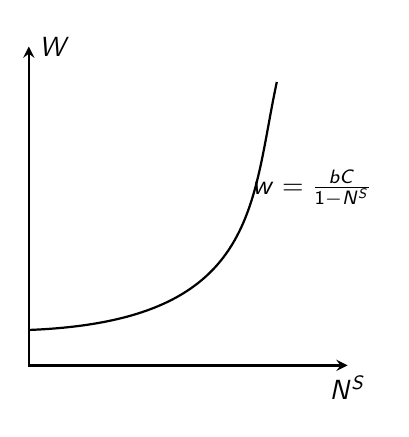
\begin{tikzpicture}[scale=0.45]
			\draw [thick, <->] (0,9) node[right]{\(W\)} -- (0,0) -- (9,0) node[below]{\(N^S\)};
			\draw [thick] (0,1) .. controls (6.5,1.25) and (6.25,4.5) .. (7,8);
			\node at (8,5) {\( w=\frac{bC}{1-N^S} \)};
		\end{tikzpicture}
		\caption{Labour supply curve}\label{fig:2.1}
	\end{marginfigure}
\subsection{Firms in the Simple RBC Model}
	\begin{itemize}
		\item Firms produce output using a production technology:
		\[
			Y = A \times (N^D)^{1-\alpha}
		\]
		\item Where \( A \) is the exogenous level of technology;
		\item And where \( N^D \) is labour inputs demanded by firms
	\end{itemize}
	\begin{marginfigure}
		\centering
		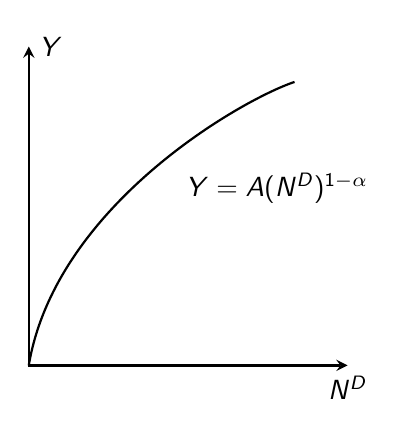
\begin{tikzpicture}[scale=0.45]
			\draw [thick, <->] (0,9) node[right]{\(Y\)} -- (0,0) -- (9,0) node[below]{\(N^D\)};
			\draw [thick] (0,0) .. controls (0.75,4.5) and (6,7.5) .. (7.5,8);
			\node at (7,5) {\( Y = A(N^D)^{1-\alpha} \)};
		\end{tikzpicture}
		\caption{Firm output curve}\label{fig:2.2}
	\end{marginfigure}
	\begin{itemize}
		\item A competitive firm chooses labour \( N^D \) to maximize profit \( \Pi \) (returned to households)
		\begin{align*}
			\Pi &= \max_{N^D} Y-wN^D\\
			&= \max_{N^D} A(N^D)^{1-\alpha} - wN^D
		\end{align*}
		\item where w is the wage or cost of hiring labour (and is taken as given)
		\item The first order condition yields:
		\[
		\underbrace{(1-\alpha)A(N^D)^{-\alpha}}_{\substack{\text{Marginal Product}\\\text{of Labour}}} - \underbrace{w}_{\substack{\text{Marginal Cost}\\\text{of Labour}}}
		\]
		\item \textcolor{myblue}{Marginal Product of Labour} (MPN) = extra output generated by one additional labour input
		\item Firms demand less labour as wages increase
		\begin{marginfigure}
			\centering
			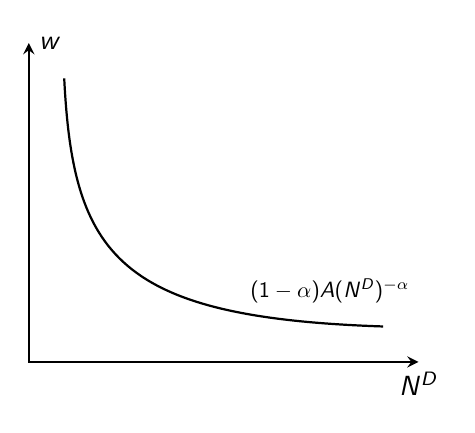
\begin{tikzpicture}[scale=0.45]
				\draw [thick, <->] (0,9) node[right]{\(w\)} -- (0,0) -- (11,0) node[below]{\(N^D\)};
				\draw [thick] (1,8) .. controls (1.25,3) and (2.5,1.25) .. (10,1);
				\node [scale = 0.8] at (8.5,2) {\( (1-\alpha) A(N^D)^{-\alpha} \)};
			\end{tikzpicture}
			\caption{The MPN curve}\label{fig:2.3}
		\end{marginfigure}
	\end{itemize}
\subsection{Equilibrium in the Simple RBC Model}
	\begin{itemize}
		\item The Labour Market clearing condition holds:
		\begin{equation}
			\frac{bC}{1-N} = w = (1-\alpha)AN^{-\alpha} \label{E:2.1}
		\end{equation}
		\item Aggregate production is determined by technology:
		\begin{equation}
			Y = AN^{1-\alpha} \label{E:2.2}
		\end{equation}
		\item Firm output (i.e. goods supply) is equal to household consumption (i.e. goods demand):
		\begin{equation}
			Y = C \label{E:2.3}
		\end{equation}
		\item First substitute \cref{E:2.3} into (\ref{E:2.2}), and substitute this into \cref{E:2.1}:
		\[
			b\frac{AN^{1-\alpha}}{1-N} = (1-\alpha)AN^{-\alpha}
		\]
		\item Second, rearrange and solve for \( N \):
		\begin{equation}
			N = \frac{(1-\alpha)}{b+(1-\alpha)}\label{E:2.4}
		\end{equation}
		\item Third, substitute into either the labour supply or demand curve to find \( w \):
		\begin{equation}
			w = (1-\alpha)A\left(\frac{(1-\alpha)}{b+(1-\alpha)}\right)^{-\alpha}\label{E:2.5}
		\end{equation}
		\item Finally use \cref{E:2.4} and (\ref{E:2.2}) and (\ref{E:2.3}) to solve for \( Y \) and \( C \):
		\begin{equation}
			Y = C = A\left(\frac{(1-\alpha)}{b+(1-\alpha)}\right)^{1-\alpha}\label{E:2.6}
		\end{equation}
	\end{itemize}
	\begin{marginfigure}
		\centering
		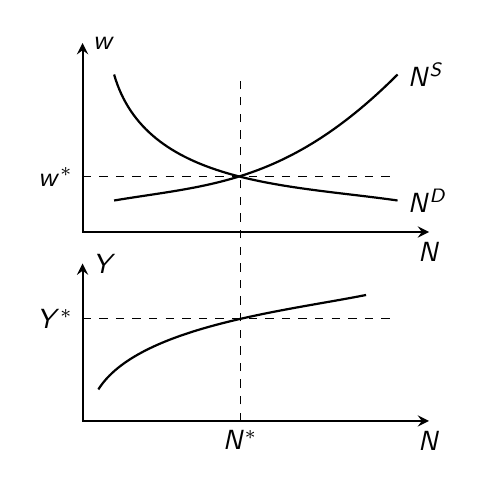
\begin{tikzpicture}[scale=0.4]
			\draw [thick, <->] (0,12) node[right]{\(w\)} -- (0,6) -- (11,6) node[below]{\(N\)};
			\draw [thick] (1,11) .. controls (2,7.5) and (6.5,7.5) .. (10,7) node [right]{\( N^D \)};
			\draw [thick] (1,7) .. controls (4,7.5) and (6.5,7.5) .. (10,11) node [right]{\( N^S \)};
			\draw [dashed] (0,7.75) node [left]{\( w^* \)} -- (10,7.75);
			\draw [thick, <->] (0,5) node[right]{\(Y\)} -- (0,0) -- (11,0) node[below]{\(N\)};
			\draw [thick] (0.5,1) .. controls (1.75,3) and (6.5,3.5) .. (9,4);
			\draw [dashed] (0,3.25) node [left]{\( Y^* \)} -- (10,3.25);
			\draw [dashed] (5,0) node [below]{\( N^* \)}-- (5,11);
		\end{tikzpicture}
		\caption{Equilibrium}\label{fig:2.4}
	\end{marginfigure}
\subsubsection{Business Cycle Fluctuations in the RBC Model}
	\begin{itemize}
		\item Macroeconomic fluctuations in early RBC models were driven entirely by changes in aggregate productivity
		\item In our simple RBC model, changes in productivity \( A \) can drive fluctuations in each of the aggregate variables: \( C,Y,w,N \)
	\end{itemize}
\subsection{Limitations of the Simple (Intra-Temporal) RBC Model}
	\begin{itemize}
		\item In our simple RBC model, households and firms only make static or intra-temporal decisions
		\item But these households do not care about the future!
		\begin{itemize}
			\item inter-temporal decisions
			\item Household savings
			\item Productive capital
			\item Financial assets (or asset prices!)
			\item A relationship between the past and the future
			\item A serious characterization of aggregate dynamics
		\end{itemize}
	\end{itemize}
\section{Inter-Temporal Choice and the Business Cycle}\label{Sec:3}
\subsection{Simple Inter-Temporal Households in the RBC Model}\label{S:3.1}
	\textbf{Choice between Consumption and Saving}
	\begin{itemize}
		\item Households must decide how much to consume today, how much to save, and how much to consume tomorrow
		\item Because savings earn interest (\textcolor{myblue}{returns}), the more resources that are saved today, the more resources are available for consumption in the future
		\item But households are impatient as they discount the value of future consumption more than the value of current consumption
		\item The optimisation problem is to maximise life-time utility subject to an \textcolor{myblue}{inter-temporal} budget constraint
	\end{itemize}
\subsubsection{A Model of Consumption and Saving}
	\begin{itemize}
		\item Assumptions:
		\begin{itemize}
			\item Earn (net) real interest rate \( r \) on savings \( S \)
			\item Future utility is discounted at the rate \( \beta \)
			Exogenous income in each period \( Y_1, Y_2 \)
		\end{itemize}
		\item Households use their savings to \textcolor{myblue}{smooth consumption across time}
		\item For now we \textcolor{myred}{ignore}:
		\begin{itemize}
			\item Risk
			\item Inflation
			\item Different types of assets
			\item Other asset market participants
		\end{itemize}
		\item A household chooses current consumption \( C_1 \), future consumption \( C_2 \), and savings \( S \):		
		\begin{alignat*}{2}
			\max_{C_1,C_2,s}\quad& \log(C_1) + \beta \log (C_2)\\
			\text{s.t.}\quad &C_1 + S = Y_1 && \text{First period budget constraint} \\
			&C_2 = Y_2 + S(1+r)\quad  && \text{Second period budget constraint}
		\end{alignat*} 
		\item Combine the within-period budget constraints:
		\[
		C_1 + \frac{C_2}{1+r} = Y_1 + \frac{Y_2}{1+r}
		\]
		\item This is the \textcolor{myblue}{inter-temporal budget constraint} (or, life-time budget constraint)
		\end{itemize}
\subsubsection{Household Choice for Consumption and Saving}
		\begin{itemize}
		\item The simplified household problem is:
		\begin{align*}
		\max_{C_1,C_2,S}\quad &\log(C_1) + \beta \log (C_2) \\
		\text{s.t.}\quad &C_1 + \frac{C_2}{1+r} = Y_1 + \frac{Y_2}{1+r}
		\end{align*}
		\item The first order condition yield:
		\begin{equation}
			\underbrace{\frac{1}{c_1}}_{\substack{\text{Marginal Utility of} \\ \text{Consumption in Period 1}}} = \underbrace{(1 + r)}_{\text{Return of Savings}} \quad\times\quad \underbrace{\beta \frac{1}{c_2}}_{\substack{\text{Marginal Utility of} \\ \text{Consumption in Period 2}}} \label{E:3.1}
		\end{equation}
		\item This is called the \textcolor{myblue}{Consumption Euler Equation}, which describes efficient inter-temporal consumption choices
		\item {Later, we will see that this equation is fundamental for understanding the price of assets!}
		\item Rearrange \cref{E:3.1} for \( C_2 \), then substitute into the inter-temporal budget constraint to find \( C_1 \) and \( C_2 \):
		\[
		C_1 = \frac{1}{1 + \beta} \left( Y_1 + \frac{Y_2}{1 + r}\right), \quad c_2 = \frac{\beta (1 + r)}{1 + \beta} \left( Y_1 + \frac{Y_2}{1 + r }\right)
		\]
		\item To find \( S \) substitute either \( C_1 \) into the first period budget constraint or \( C_2 \) into the second period budget constraint:
		\[
		S = \frac{\beta}{1 + \beta} Y_1 - \frac{1}{( 1 + r )(1 + \beta)} Y_2
		\]
		\item  Rewrite the savings function for \( r \):
		\[
		r = \frac{Y_2}{\beta Y_1 - (1 + \beta)S} - 1
		\]
		\item This represents the household's \textcolor{myblue}{supply of savings}
	\end{itemize}
	\begin{marginfigure}
		\centering
		\begin{tikzpicture}[scale=0.45]
			\draw [thick, <->] (0,9) node[left]{\(r\)} -- (0,0) -- (9,0) node[below]{\(S\)};
			\draw [thick] (0,1) .. controls (6.5,1.25) and (5.75,4.5) .. (6,8);
			\node [scale =0.8] at (8,5) {\( \frac{Y_2}{\beta Y_1 - (1 + \beta)S} - 1 \)};
		\end{tikzpicture}
		\caption{Household Savings}\label{fig:3.1}
	\end{marginfigure}
	\begin{itemize}
		\item When does the household choose to save (i.e. S > 0)?
		\begin{itemize}
			\item Save when income in period 1 \( (Y_1) \) is larger than income in period 2 \( (Y_2) \)
			\item Save more when the interest rate r is high
		\end{itemize}
		\item What makes saving valuable?
		\item Savings transfers resources from periods of high income (when the MU of consumption is low) to periods of low income (when the MU of consumption is high)
	\end{itemize}
\subsection{Inter-Temporal Households and Capital Accumulation in the RBC Model}\label{S:3.2}
	\begin{itemize}
		\item Inter-temporal households generate a supply of savings (or a demand for loans!)
		\item In the canonical RBC model, households hold physical capital that is then used in production
		\item Here, we want to think of capital as a \textcolor{myblue}{productive asset}, but one whose return may fluctuate with the business cycle
	\end{itemize}
\subsubsection{Household Consumption Choice and Capital Accumulation}
	\begin{itemize}
		\item A household chooses current consumptions \( C_1, C_2, \) and investment in capital \( I_1 \):
		\begin{alignat*}{2}
			\max_{C_1,C_2,I_1}\quad &\log(C_1) + \beta \log (C_2) \\
			\text{s.t.}\quad &C_1 + I_1 = \Pi_1 + r_1 K_1 && \text{First period budget constraint} \\
			&C_2 = \Pi_2 + (1 + r_2 - \delta)K_2\quad  && \text{Second period budget constraint} \\
			&K_2 = I_1 + K_1 (1 - \delta) && \text{Capital accumulation equation}
		\end{alignat*}
		\item Households are endowed with capital \( K_1 \) (cannot be adjusted)
		\item Households earn (net) real interest \( r_1, r_2 \) on their capital holdings
		\item Capital in period 2 is investment in new capital + undepreciated capital from period 1
		\item In period 2, after production takes place, households consume remaining capital: \( (1 - \delta)K_2 \)
		\item For simplicity, assume households don't supply labour, but they own firms and receive dividends \( \Pi_1, \Pi_2 \)
		\item Substitute capital accumulation equation into first period budget constraint:
		\[
		C_1 + K_2 = \Pi_1 + K_1 (1 + r_1 - \delta)
		\]
		\item Now, substitute the budget constraints into the utility function:
		\[
		\max_{K_2} \log (\Pi_1 + K_1 (1+ r_1 - \delta) - K_2) + \beta \log (\Pi_2 + K_2 (1 + r_2 - \delta))
		\]
		\item Taking the FOC with respect to \( K_2 \):
		\[
		\frac{1}{c} = \beta (1 + r_2 - \delta) \frac{1}{c_2}
		\]
		\item Which is also a \textcolor{myblue}{Consumption Euler Equation}
		\item Here, the return on savings/capital holding is \( (1 + r_2 - \delta) \), but households value capital in the same way they valued savings in \cref{S:3.1}
	\end{itemize}
	\begin{marginfigure}
		\centering
		\begin{tikzpicture}[scale=0.45]
			\draw [thick, <->] (0,9) node[left]{\(r_2\)} -- (0,0) -- (9,0) node[below]{\(K_2\)};
			\draw [thick] (0,0.75) .. controls (7.5,1) and (7,4.5) .. (7.5,8);
			\node at (8.5,7) {\( K_2^{\text{supply}} \)};
		\end{tikzpicture}
		\caption{Household capital Accumulation}\label{fig:3.2}
	\end{marginfigure}
\subsection{Firms in the Inter-Temporal RBC Model}
	\begin{itemize}
		\item Firms produce output using the production technology:
		\[
		Y_t = A_t K_t^\alpha , \text{where } t = 1,2
		\]
		\item Where \( A_t \) is technology/productivity; and \( K_t \) is the capital inputs of firms
	\end{itemize}
	\begin{marginfigure}
		\centering
		\begin{tikzpicture}[scale=0.45]
			\draw [thick, <->] (0,9) node[left]{\(Y_t\)} -- (0,0) -- (9,0) node[below]{\(K_t\)};
			\draw [thick] (0,0) .. controls (0.25,5.5) and (6,5.75) .. (7.5,6);
			\node at (8,6.5) {\( A_t K_t^\alpha \)};
		\end{tikzpicture}
		\caption{Firms capital Accumulation}\label{fig:3.3}
	\end{marginfigure}
\subsubsection{Firm's Choice of Capital Inputs}
	\begin{itemize}
		\item A competitive firm chooses capital \( K_2^D \) to maximise profit \( \Pi_2 \):
		\[
		\Pi_2 = \max_{K_2^D} A_2(K_2^D)^\alpha - r_2K_2^D
		\]
		\item where \( r_2 \) is the interest rate or rental rate of capital (taken as given)
		\item The first order condition yields:
		\[
		\underbrace{\alpha A_2 (K_2^D)^{\alpha - 1}}_{\substack{\text{Marginal Utility} \\ \text{of Capital}}} \ - \: \underbrace{r_2}_{\substack{\text{Marginal Cost} \\ \text{of Capital}}} = 0
		\]
		\item \textcolor{myblue}{Marginal Product of Capital} (MPK) = extra output generated by additional capital input
		\item The FOC yields the capital demand curve:
		\[
		r_2 = \alpha A_2 (K_2^D)^{\alpha-1}
		\]
	\end{itemize}
	\begin{marginfigure}
		\centering
		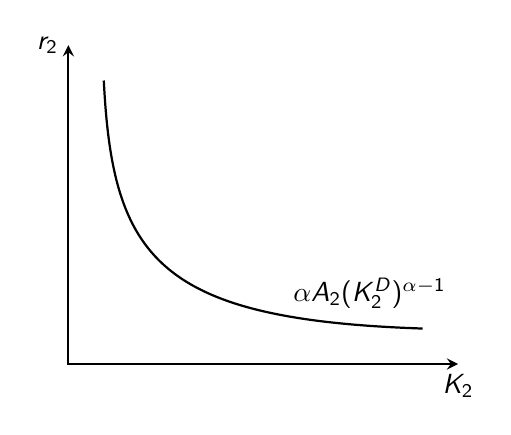
\begin{tikzpicture}[scale=0.45]
			\draw [thick, <->] (0,9) node[left]{\(r_2\)} -- (0,0) -- (11,0) node[below]{\(K_2\)};
			\draw [thick] (1,8) .. controls (1.25,3) and (2.5,1.25) .. (10,1);
			\node at (8.5,2) {\( \alpha A_2 (K_2^D)^{\alpha-1} \)};
		\end{tikzpicture}
		\caption{MPK}\label{fig:3.4}
	\end{marginfigure}
\subsubsection{Firm's Profits}
	\begin{itemize}
		\item Recall that households own the firms and receive the profits the firms generate:
		\begin{alignat*}{2}
			\text C_1 + I_1 & = \Pi_1 + r_1 K_1 && \text{First period budget constraint} \\
			C_2 & = \Pi_2 + (1 + r_2 - \delta) K_2  &\quad& \text{Second period budget constraint} \\
		\end{alignat*}
		\item The firms' first order condition gives us \( r_t = \alpha A_t (K_t^D)^{\alpha - 1} \), so profits are:
		\begin{align*}
		\Pi_t & = A_t (K_t^D)\alpha - r_t K_t^D \\
		& = A_t (K_t^D)\alpha - \alpha A_t (K_t^D)^{\alpha - 1} K_t^D \\
		& = A_t (K_t^D)\alpha - \alpha A_t (K_t^D)^\alpha \\
		& = (1-\alpha) A_t (K_t^D)^\alpha > 0
		\end{align*}
		\item Which means households are sensitive to changes in productivity \textit{through} their ownership of firms
	\end{itemize}
\subsection{Equilibrium in the Inter-Temporal RBC Model}
	\begin{itemize}
		\item The \textcolor{myblue}{Capital Market} clearing condition holds:
		\begin{itemize}
			\item The real interest rate \( r_t \) ensures that the capital market clears
			\item Capital supply (by households) is equal to capital demand (by firms) \( K_t^S = K_t^D \)
		\end{itemize}
		\item Aggregate production is determined by technology:
		\begin{equation}
			Y_t = A_t K_t^\alpha , t =1,2
		\end{equation}
		\item The aggregate resource constraint holds each period:
		\begin{gather}
			Y_1 = C_1 + I_1 \\
			Y_2 + ( 1 - \delta ) K_2 = C_2
		\end{gather}
		\item (Where total resources in period 2 include remaining undepreciated capital)
	\end{itemize}
	\begin{itemize}
		\item Notice the \textcolor{myblue}{real economy} is tightly linked to the \textcolor{myblue}{asset market} (i.e. capital market) \item Equilibrium return on assets (i.e. interest rate), pins down amount of capital supplied \item Capital supply determines production/output in the economy
		\item So the macroeconomy and asset markets are very closely related!
	\end{itemize}
	\begin{marginfigure}
		\centering
		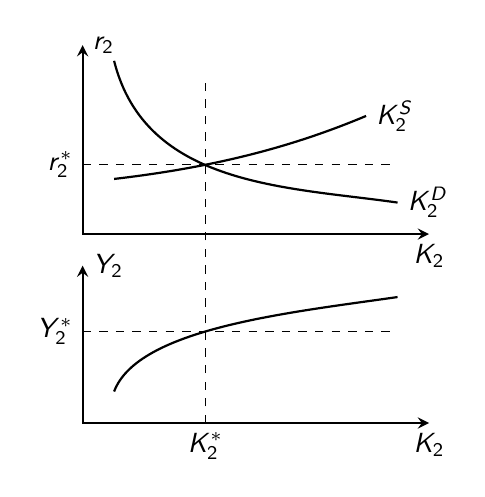
\begin{tikzpicture}[scale=0.4]
			\draw [thick, <->] (0,12) node[right]{\(r_2\)} -- (0,6) -- (11,6) node[below]{\(K_2\)};
			\draw [thick] (1,11.5) .. controls (2,7.5) and (6.5,7.5) .. (10,7) node [right]{\( K_2^D \)};
			\draw [thick] (1,7.75) .. controls (4,8.1) and (6.5,8.7) .. (9,9.75) node [right]{\( K_2^S \)};
			\draw [dashed] (0,8.2) node [left]{\( r_2^* \)} -- (10,8.2);
			\draw [thick, <->] (0,5) node[right]{\(Y_2\)} -- (0,0) -- (11,0) node[below]{\(K_2\)};
			\draw [thick] (1,1) .. controls (1.75,3) and (6.5,3.5) .. (10,4);
			\draw [dashed] (0,2.9) node [left]{\( Y_2^* \)} -- (10,2.9);
			\draw [dashed] (3.9,0) node [below]{\( K_2^* \)}-- (3.9,11);
		\end{tikzpicture}
		\caption{Equilibrium}\label{fig:3.5}
	\end{marginfigure}
\subsubsection{RBC Model Implications}
	\begin{itemize}
		\item Business cycles are due to ``real'' shocks (e.g. TFP or technology shocks)
		\item Productivity, real wages, employment, consumption, and investment are all pro-cyclical
		\item Markets are always in equilibrium.
		\item Prices and wages always adjust (flexibly) to ensure this equilibrium is efficient
		\item No involuntary unemployment in the model
		\item Money neutrality holds: changes in money supply do not affect real variables
		\item Government stabilization policies tend to be counter-productive
	\end{itemize}
\subsection{Limitations of RBC Models}
	\begin{itemize}
		\item How do we measure TFP shocks? Solow Residuals?
		\item Do we really have frequent regressions in technological progress that cause recessions?
		\item What is the role of fiscal and monetary policy in the evolution of the macroeconomy?
		\item Most macroeconomists now convinced that money neutrality only holds in the \textcolor{myblue}{long run}
		\item Real wages are \textcolor{myred}{not} pro-cyclical in the data. What does this imply?
		\begin{itemize}
			\item ``Real Wages and the Business Cycle'', Abraham and Haltiwanger (JEL, 1995)
			\item ``Short-Run Equilibrium Dynamics of Unemployment, Vacancies, and Real Wages'', Pissarides, (AER, 1985)
		\end{itemize}
		\item To answer these questions, will typically need a DSGE model that incorporates price stickiness, wage stickiness, and policy shocks
		\item Most models in the RBC literature are solved using \textcolor{myred}{linear approximations} to the model
		\item These linear approximations study deviations of the model from a well-defined \textcolor{myblue}{steady state} of the model economy
		\item But linear approximation means agents solve their problems under \textcolor{myred}{certainty equivalence}:
		\item Certainty equivalence \( \Longleftrightarrow \) agents behave as if there is \textcolor{myred}{no risk}!
		\item But risk is one of the primary reasons for holding financial assets:
		\begin{itemize}
			\item We often want to insure against risks by holding financial assets that pay out if certain undesirable states of the world eventuate (e.g. unemployment, fire, theft, death)
			\item In equilibrium, agents often want to share or smooth risks e.g. you payout when I am doing poorly, and I payout when you are doing poorly
		\end{itemize}
	\end{itemize}
\section{Money and Savings in the New Keynesian Model}\label{Sec:4}
\subsection{An Introduction to the New Keynesian Model}
	\begin{itemize}
		\item The ideas of John Maynard Keynes dominated macroeconomics in the early 20th century
		\item Keynesian macroeconomics (e.g. the IS-LM-AS model) studied government policies that might stabilize output in response to shocks
		\item The RBC model, with its lack of government stabilisation policy, dominated macroeconomics from the 1970s
		\item But continuing to believe in the importance of government policy, macroeconomists then developed what is now called the \textcolor{myblue}{New Keynesian Model}
		\item Like the RBC model, the \textcolor{myblue}{New Keynesian Model}:
		\begin{itemize}
			\item Has micro foundations of economic behaviour
			\item Has agents with rational expectations about the future
			\item Can be calibrated to match various business cycle statistics about the macroeconomy
		\end{itemize}
		\item Unlike the RBC model, the \textcolor{myblue}{New Keynesian Model}:
		\begin{itemize}
			\item Features price and/or wages that are sticky (i.e. do not update in response to economic shocks)
			\item Describes a macroeconomy that does not respond efficiently to shocks
			\item May lead to output and employment being far from their socially optimal levels
			\item Allows a role for macroeconomic stabilisation via monetary policy and/or fiscal policy
		\end{itemize}
	\end{itemize}
\subsection{Inflation, and Nominal and Real Interest Rates}
\subsubsection{Inflation}
	\begin{itemize}
		\item Define the general price level in an economy: \( P_t \equiv \) price index
		\begin{itemize}
			\item i.e the dollar cost of a representative basket of consumer goods
		\end{itemize}
		\item Inflation: \( \pi \equiv \) percent change in the price index:
		\begin{align*}
			\pi_t &= \frac{P_t - P_{t-1}}{P_{t-1}}\\
			&= \frac{P_t}{P_{t-1}} - 1
		\end{align*}
	\end{itemize}
	\begin{figure}[H]\centering
		\begin{tikzpicture}
			\begin{axis}[
				title = {International Inflation Rates},
				axis on top,
				no markers,
				height = \axisdefaultheight,
				width = 0.95\textwidth,
				date coordinates in = x,
				date ZERO = {1960-01-01},
				xticklabel = {\year},
				xtick = {
					1960-01-01,
					1970-01-01,
					1980-01-01,
					1990-01-01,
					2000-01-01,
					2010-01-01,
					2020-01-01
				},
				xmin = 1960-01-01,
				xmax = 2022-01-01,
				xtick pos = left, 
				xtick align = outside,
				ylabel = {Inflation Rate (Annual, \%)},
				ytick = {0,5,10,15,20,25},
				ytick pos = bottom,
				ytick align = outside,
				ymin = -3,
				ymax = 28,
				legend pos = north east,
				legend cell align = left,
				legend style = {font=\scriptsize,draw=none,fill opacity=0.75,cells={align=left}},
				legend entries = {US,UK,Japan,Australia,New Zealand},
				]
				\addplot+[color=myblue,thick,smooth] table [x=Date,y=US,col sep=comma] {International-Inflation.csv};
				\addplot+[color=mypurple,thick,smooth] table [x=Date,y=UK,col sep=comma] {International-Inflation.csv};
				\addplot+[color=myred,thick,smooth] table [x=Date,y=Japan,col sep=comma] {International-Inflation.csv};
				\addplot+[color=mygold,thick,smooth] table [x=Date,y=AUS,col sep=comma] {International-Inflation.csv};
				\addplot+[color=mygreen,thick,smooth] table [x=Date,y=NZ,col sep=comma] {International-Inflation.csv};
				\addplot [black, no markers] coordinates {(1960-01-01,0) (2022-04-01,0)};
			 \end{axis}
			\end{tikzpicture}
		\label{fig:4.1}
	\end{figure}
\subsubsection{Definitions of Nominal Variables}
	\begin{itemize}
		\item Nominal interest rate: \( r_t^n \equiv \) \textcolor{myblue}{rate of return} on an asset, in period \( t \) dollars
		\item Asset price: \( S_t \equiv \) dollar price of a discount bond that pays one dollar next period
		\begin{itemize}
			\item Discount bond: a bond that is issued or traded at less than its face--value
			\item Face-value: amount the bond issuer pays to the bondholder once maturity is reached
			\item Maturity: length of time a bond is held e.g. one month, one quarter, a year
		\end{itemize}
		\item If \( r_n^t \) is the rate of return on the discount bond, then we we compute this as:
	\end{itemize}
	\begin{align*}
		r_t^n &= \frac{\text{Payoff}_{t+1} - \text{Bond Price}_t}{\text{Bond Price}_t}\\
		&= \frac{1 - S_t}{S_t} = \frac{1}{S_t} - 1\\
		\Rightarrow \: S_t &= \frac{1}{r_t^n}
	\end{align*}
\subsubsection{Real vs. Nominal Interest Rates and the Fisher Equation}
	\begin{itemize}
		\item Purchasing power of one dollar \( \equiv \frac{1}{P_t} \)
		\begin{itemize}
			Purchasing power represents the number of consumption goods one dollar can buy
		\end{itemize}
		\item The ``ex-post'' real interest rate \( r_t \equiv \) realised return on the bond in units of consumption:
		\begin{align*}
			r_t &= \frac{\frac{1}{P_{t+1}} - \frac{S_t}{P_t}}{\frac{S_t}{P_t}} = \frac{1}{S_t}\frac{P_t}{P_{t+1}} - 1\\
			\Rightarrow \: 1 + r_t &= \frac{1+r_t^n}{1+\pi_{t+1}}
		\end{align*}
		\item Rearranging
		\begin{align*}
			1 + r_t^n &= (1 + r_t)(1 + \pi_{t+1})\\
			&= 1 + r_t + \pi_{t+1} + r_t \pi_{t+1}
		\end{align*}
		\item Since \( r_t \pi_{t+1} \approx 0 \) for small values of \( r_t \) and \( \pi_{t+1} \):
		\[
			r_t^{} \approx r_t^n - \pi_{t+1}^{}
		\]
		\item Which is known as the \textcolor{myblue}{Fisher Equation}
	\end{itemize}
\subsubsection{Expected vs. Ex-Post Real Interest Rate}
	\begin{itemize}
		\item The \textcolor{myblue}{expected} real rate is \( E_t(r_t): \)
		\[
			E_t(r_t)^{} \approx E_t(r_t^n) - E_t^{}(\pi_{t+1}) = r_t^n - E_t^{}(\pi_{t+1}^{})
		\]
	\end{itemize}
	\begin{center}
	\begin{tabular}{cc}
		\begin{tikzpicture}[baseline]
			\begin{axis}[
				title = {US},
				axis on top,
				no markers,
				date coordinates in = x,
				date ZERO = {1960-01-01},
				xticklabel = {\year},
				xtick = {
					1960-01-01,
					1970-01-01,
					1980-01-01,
					1990-01-01,
					2000-01-01,
					2010-01-01,
					2020-01-01
				},
				xmin = 1960-01-01,
				xmax = 2022-04-01,
				xtick pos = left,
				xtick align = outside,
				ytick = {0,10,20,30},
				ytick pos = bottom,
				ytick align = outside,
				yticklabel style={overlay},
				ymin = -2,
				ymax = 30,
				legend pos = north east,
				legend cell align = left,
				legend style = {font=\scriptsize,draw=none,fill opacity=0.75,cells={align=left}},
				legend entries = {Nominal Rate, Inflation},
				]
				\addplot+[color=myblue,thick,smooth] table [x=Date,y=US-Rate,col sep=comma] {InterestRate-Inflation.csv};
				\addplot+[color=myred,thick,smooth] table [x=Date,y=US-Inflation,col sep=comma] {InterestRate-Inflation.csv};
				\addplot [black, no markers] coordinates {(1960-01-01,0) (2022-04-01,0)};
			\end{axis}
		\end{tikzpicture}
	&
		\begin{tikzpicture}[baseline]
			\begin{axis}[
				title = {UK},
				axis on top,
				no markers,
				date coordinates in = x,
				date ZERO = {1960-01-01},
				xticklabel = {\year},
				xtick = {
					1960-01-01,
					1970-01-01,
					1980-01-01,
					1990-01-01,
					2000-01-01,
					2010-01-01,
					2020-01-01
				},
				xmin = 1960-01-01,
				xmax = 2022-04-01,
				xtick pos = left,
				xtick align = outside,
				ytick = {0,10,20,30},
				ytick pos = bottom,
				ytick align = outside,
				yticklabel style={overlay},
				ymin = -2,
				ymax = 30,
				legend pos = north east,
				legend cell align = left,
				legend style = {font=\scriptsize,draw=none,fill opacity=0.75,cells={align=left}},
				legend entries = {Nominal Rate, Inflation},
				]
				\addplot+[color=myblue,thick,smooth] table [x=Date,y=UK-Rate,col sep=comma] {InterestRate-Inflation.csv};
				\addplot+[color=myred,thick] table [x=Date,y=UK-Inflation,col sep=comma] {InterestRate-Inflation.csv};
				\addplot [black, no markers,smooth] coordinates {(1960-01-01,0) (2022-04-01,0)};
			\end{axis}
		\end{tikzpicture}
	\\
		\begin{tikzpicture}[baseline]
			\begin{axis}[
				title = {Australia},
				axis on top,
				no markers,
				date coordinates in = x,
				date ZERO = {1961-01-01},
				xticklabel = {\year},
				xtick = {
					1960-01-01,
					1970-01-01,
					1980-01-01,
					1990-01-01,
					2000-01-01,
					2010-01-01,
					2020-01-01
				},
				xmin = 1960-01-01,
				xmax = 2022-04-01,
				xtick pos = left,
				xtick align = outside,
				ytick = {0,10,20,30},
				ytick pos = bottom,
				ytick align = outside,
				yticklabel style={overlay},
				ymin = -2,
				ymax = 30,
				legend pos = north east,
				legend cell align = left,
				legend style = {font=\scriptsize,draw=none,fill opacity=0.75,cells={align=left}},
				legend entries = {Nominal Rate, Inflation},
				]
				\addplot+[color=myblue,thick,smooth] table [x=Date,y=AUS-Rate,col sep=comma] {InterestRate-Inflation.csv};
				\addplot+[color=myred,thick,smooth] table [x=Date,y=AUS-Inflation,col sep=comma] {InterestRate-Inflation.csv};
				\addplot [black, no markers] coordinates {(1960-01-01,0) (2022-04-01,0)};
			\end{axis}
		\end{tikzpicture}
	&
		\begin{tikzpicture}[baseline]
			\begin{axis}[
				title = {New Zealand},
				axis on top,
				no markers,
				date coordinates in = x,
				date ZERO = {1960-01-01},
				xticklabel = {\year},
				xtick = {
					1960-01-01,
					1970-01-01,
					1980-01-01,
					1990-01-01,
					2000-01-01,
					2010-01-01,
					2020-01-01
				},
				xmin = 1960-01-01,
				xmax = 2022-04-01,
				xtick pos = left,
				xtick align = outside,
				ytick = {0,10,20,30},
				ytick pos = bottom,
				ytick align = outside,
				yticklabel style={overlay},
				ymin = -2,
				ymax = 30,
				legend pos = north east,
				legend cell align = left,
				legend style = {font=\scriptsize,draw=none,fill opacity=0.75,cells={align=left}},
				legend entries = {Nominal Rate, Inflation},
				]
				\addplot+[color=myblue,thick,smooth] table [x=Date,y=NZ-Rate,col sep=comma] {InterestRate-Inflation.csv};
				\addplot+[color=myred,thick,smooth] table [x=Date,y=NZ-Inflation,col sep=comma] {InterestRate-Inflation.csv};
				\addplot [black, no markers] coordinates {(1960-01-01,0) (2022-04-01,0)};
			\end{axis}
		\end{tikzpicture}
	\\
	\end{tabular}
	\end{center}
\subsection{Money and Inflation}
\subsubsection{The Rate of Return on Money}
	\begin{itemize}
		\item We can also think of \textcolor{myblue}{money} as a type of asset.
		\item But what is the rate of return on money?
		\begin{itemize}
			\item Since the nominal rate of return on money is \( r_{m,t}^n = 0 \), the real return is:
			\begin{align*}
				r_{m,t}^{} - r_{m,t}^n - E_t^{}(\pi_{t+1}^{})
			\end{align*}
		\end{itemize}
			\item \textbf{The return on money falls as expected inflation rises}
			\item So why do people hold money when its return is much lower than other assets?
		\begin{itemize}
			\item Convenience: money has a role as a \textcolor{myblue}{medium of exchange} (i.e. used for trading goods and services)
			\item Risk: fear of bank failures/financial market collapse (e.g. ``money under the mattress'')
		\end{itemize}
	\end{itemize}
\subsubsection{Returns on Money vs. Bonds}
	\begin{itemize}
		\item Recall:
		\begin{itemize}
			\item Real rate of return on money:
			\[
				r_{m,t}^{} = -E_t^{}(\pi_{t+1}^{})
			\]
			\item (Expected) real rate of return on bonds:
			\[
				E_t^{}(r_t^{}) \approx r_t^n - E_t^{}(\pi_{t+1}^{})
			\]
	\end{itemize}	
		\item Assuming the Fisher Hypothesis (i.e. that nominal rates move with inflation)
		\item Then fluctuations in inflation change return on money relative to the return on bonds
		\item Therefore, when monetary policy influences inflation, also \textcolor{myblue}{affects the incentive to hold different kinds of assets}
	\end{itemize}
\subsubsection{Quantity Theory of Money}
	\begin{itemize}
		\item Consider again the Fisher Hypothesis:
		\[
			r_t^n \approx E_t^{} (r_t^{}) + E_t^{} (\pi_{t+1}^{})
		\]
		\item If nominal interest rates move with inflation, what drives inflation?
		\item Much empirical evidence suggests a link between money growth and inflation
		\begin{itemize}
			\item Evidence across time within a given country (mainly evidence over the long-run)
			\item Evidence across countries
		\end{itemize}
	\end{itemize}
	\begin{figure}[H]
	\begin{tikzpicture}
		\begin{axis}[
			title = {Inflation and Money Growth (USA)},
			axis on top,
			no markers,
			height = \axisdefaultheight,
			width = 0.95\textwidth,
			date coordinates in = x,
			date ZERO = {1960-01-01},
			xticklabel = {\year},
			xtick = {
				1960-01-01,
				1970-01-01,
				1980-01-01,
				1990-01-01,
				2000-01-01,
				2010-01-01,
				2020-01-01
			},
			xmin = 1960-01-01,
			xmax = 2022-04-01,
			xtick pos = left,
			xtick align = outside,
			ylabel = {Growth Rate (Annual, \%)},
			ytick = {-2.5,0,2.5,5,7.5,10,12.5,15},
			ytick pos = bottom,
			ytick align = outside,
			ymin = -4,
			ymax = 15,
			legend pos = north east,
			legend cell align = left,
			legend style = {font=\scriptsize,draw=none,fill=none,cells={align=left}},
			legend entries = {Inflation,\( \Delta \) M2},
			]
			\addplot+[color=myred,thick,smooth] table [x=Date,y=Inflation,col sep=comma] {USA-Inflation-Money.csv};
			\addplot+[color=myblue,thick,smooth] table [x=Date,y=M2,col sep=comma] {USA-Inflation-Money.csv};
			\addplot [black, no markers] coordinates {(1960-01-01,0) (2022-04-01,0)};
		\end{axis}
	\end{tikzpicture}
	\end{figure}
	\begin{itemize}
		\item Irving Fisher developed the \textcolor{myblue}{Quantity Theory of Money} (QTM):
		\begin{itemize}
			\item A theory of the price level that explains what determines the value of a unity of money
		\end{itemize}
		\item Begin with an accounting identity:
		\[
			expenditures \equiv receipts
		\]
		\item Let \( M \equiv \) stock of money; \( V \equiv \) velocity of money (i.e. number of times a unit of money changes hands per period); \( Y \equiv \) real output
		\item Then:
		\begin{align*}
			M \times V &= expenditures \\
			P \times Y &= receipts \\
			\Rightarrow MV &= PY
		\end{align*}
		\item tart with the Quantity theory identity:
		\begin{align*}
			M_t V_t &= P_t Y_t \\
			\Rightarrow \Delta \ln M_t + \Delta \ln V_t &= \Delta \ln P_t + \Delta \ln Y_t
		\end{align*}
		\item Rearranging:
		\[
			\Delta \ln P_t = \Delta \ln M_t + \Delta \ln V_t - \Delta \ln Y_t
		\]
		\item The Quantity Theory then states:
		\begin{itemize}
			\item Assumption (1) \( \Delta \ln Y_t \) is independent of \( \Delta \ln P_t, \Delta \ln M_t, \Delta \ln V_t \) (i.e. neo-classical assumption of \textbf{\textcolor{myblue}{monetary neutrality}})
			\item Assumption (2) \( \Delta \ln V_t = 0 \)
		\[
			\Rightarrow \Delta \ln P_t = \Delta \ln M_t - \Delta \ln Y_t
		\]
		\end{itemize}		
	\end{itemize}
	\begin{enumerate}[label=\textbf{\arabic*.}]
		\item Why assume \( Y \) is independent of \( M,P,V \)?
		\begin{itemize}
			\item Neo-Classical theory argues only real factors matter for Y (e.g. technology)
		\end{itemize}
		\item Why assume stable velocity of money?
		\begin{itemize}
			\item Fisher assumed money demand was proportional to nominal income:
			\begin{align*}
				M &= \kappa PY \\
				\Rightarrow M \frac{1}{\kappa} &= PY \\
				\Rightarrow V &= \frac{1}{\kappa}, \text{so V is constant}
			\end{align*}
		\end{itemize}
	\end{enumerate}
	\begin{itemize}
		\item This might be true if financial institutions and technologies change slowly over time
	\end{itemize}
	\begin{enumerate}[label=\textbf{\arabic*.}]
		\item \( Y \) is independent of \( M,P,V \)? \textcolor{myred}{NO!}
		\begin{itemize}
			\item Much evidence shows that \( Y \) is clearly not independent of \( M \)
			\item Periods when central banks have sharply contracted the money supply have been followed by large real output declines
			\begin{itemize}
				\item E.g.: Great Depression of the 1930s; large disinflations of the 1980s/1990s
			\end{itemize}
			\item Why? Temporary \textbf{nominal price rigidities} mean M affects Y in short run
			\begin{itemize}
				\item If P is \textcolor{myblue}{sticky} in the short run, then variation in M will affect Y
			\end{itemize}
		\end{itemize}
		\[
			Y = V \times \underbrace{\frac{M}{P}}_{\substack{\text{Real Money} \\ \text{Supply}}}
		\]
	\end{enumerate}
	\begin{figure*}[H]
	\centering
	\begin{tikzpicture}[baseline]
		\begin{axis}[
			title = {US},
			axis on top,
			no markers,
			date coordinates in = x,
			date ZERO = {1960-01-01},
			xticklabel = {\year},
			xtick = {
				1960-01-01,
				1970-01-01,
				1980-01-01,
				1990-01-01,
				2000-01-01,
				2010-01-01,
				2020-01-01
			},
			xmin = 1960-01-01,
			xmax = 2022-04-01,
			ylabel = {Growth Rate (Annual, \%)},
			ylabel style = {overlay},
			xtick pos = left,
			xtick align = outside,
			ytick = {-10,-5,0,5,10,15,20,25,30},
			ytick pos = bottom,
			ytick align = outside,
			ymin = -11,
			ymax = 30,
			legend pos = north east,
			legend cell align = left,
			legend style = {font=\scriptsize,draw=none,fill opacity=0.75,cells={align=left}},
			legend entries = {\( \Delta \) GDP,\( \Delta \) M2},
			]
			\addplot+[color=myblue,thick,smooth] table [x=Date,y=USA-GDP,col sep=comma] {RealGDP-Money.csv};
			\addplot+[color=myred,thick,smooth] table [x=Date,y=USA-M2,col sep=comma] {RealGDP-Money.csv};
			\addplot [black, no markers] coordinates {(1960-01-01,0) (2022-04-01,0)};
		\end{axis}
	\end{tikzpicture}
	\begin{tikzpicture}[baseline]
		\begin{axis}[
			title = {Australia},
			axis on top,
			no markers,
			date coordinates in = x,
			date ZERO = {1960-01-01},
			xticklabel = {\year},
			xtick = {
				1960-01-01,
				1970-01-01,
				1980-01-01,
				1990-01-01,
				2000-01-01,
				2010-01-01,
				2020-01-01
			},
			xmin = 1960-01-01,
			xmax = 2022-04-01,
			xtick pos = left,
			xtick align = outside,
			ylabel style = {inner sep=0pt},
			ytick = {-10,-5,0,5,10,15,20,25,30},
			ytick pos = bottom,
			ytick align = outside,
			ymin = -11,
			ymax = 30,
			legend pos = north east,
			legend cell align = left,
			legend style = {font=\scriptsize,draw=none,fill opacity=0.75,cells={align=left}},
			legend entries = {\( \Delta \) GDP,\( \Delta \) M3},
			]
			\addplot+[color=myblue,thick,smooth] table [x=Date,y=AUS-GDP,col sep=comma] {RealGDP-Money.csv};
			\addplot+[color=myred,thick,smooth] table [x=Date,y=AUS-M3,col sep=comma] {RealGDP-Money.csv};
			\addplot [black, no markers] coordinates {(1960-01-01,0) (2022-04-01,0)};
		\end{axis}
	\end{tikzpicture}
	\end{figure*}
	\begin{enumerate}[resume]
		\item Stable velocity of money? \textcolor{myred}{NO!}
		\begin{itemize}
			\item Velocity is not constant and appears to be strongly pro-cyclical
			\item Problem:
			\begin{itemize}
				\item Changes in financial technology provide easier to access money/substitutes (e.g. on-call savings accounts, EFTPOS, Pay-Wave), which changes velocity
				\item The opportunity cost of holding money - i.e. the nominal interest rate on other assets \( r_t^n \) - also matters
				\item Empirically, money demand does not have a simple proportional relationship to output
			\end{itemize}
		\end{itemize}
	\end{enumerate}
\subsection{A Simple New Keynseian Model}
	\begin{itemize}
		\item Household chooses consumption, nominal bonds, and \textcolor{myblue}{money}
		\item Simplified demand for money due to \textcolor{myblue}{utility of holding real money balances}
		\begin{itemize}
			\item Represents the ``convenience yield'' of money holdings
			\item But is something of a short-cut to characterize various desires for holding money
		\end{itemize}
	\end{itemize}
\subsubsection{Household Choice Problem}
	\begin{itemize}
		\item Household choice problem is:
		\begin{align*}
			\max_{C_1,C_2,M_1,B_2}\quad &\log(C_1) + \omega \log \frac{M_1}{P_1} + \beta \log (C_2) \\
			\text{s.t.}\quad & P_1 C_1 + M_1 + B_2 = P_1 Y_1 \\
			&P_2 C_2 = P_2 Y_2 + M_1 + B_2 (1 + r^n)
		\end{align*} 
		\item Where \( M_1/P_1 \) are real money balances
		\item The inter-temporal real budget constraint is:
		\[
			C_1 + \frac{M_1}{P_1} + \frac{C_2}{1+r^n} \frac{P_2}{P_1} = Y_1 + \frac{Y_2}{1+r^n} \frac{P_2}{P_1} + \frac{M_1/P_1}{1+r^n}
		\]
		\item The Lagrangian Problem is:
		\[
			\mathcal{L} = \log(C_1) + \omega \log \frac{M_1}{P_1} + \beta \log (C_2) + \lambda \left( Y_1 + \frac{Y_2}{1+r^n} \frac{P_2}{P_1} + \frac{M_1/P_1}{1+r^n} - C_1 - \frac{M_1}{P_1} - \frac{C_2}{1+r^n} \frac{P_2}{P_1} \right) 
		\]
		\item The first order conditions for the problem are:
		\begin{align*}
			C_1:\quad &\frac{1}{C_1} - \lambda = 0 \\
			C_2:\quad &\beta \frac{1}{C_2} - \lambda \frac{1}{1+r^n} \frac{P_2}{P_1} = 0 \\
			M_1:\quad & \omega \frac{1}{P_1} \frac{1}{M_1/P_1} + \lambda \frac{1}{1+r^n} \frac{1}{P_1} - \lambda \frac{1}{P_1} = 0
		\end{align*}
		\item Combining the first two yields the \textcolor{myblue}{consumption Euler equation}:
		\[
			\frac{1}{C_1} = \beta (1 + r^n) \frac{P_1}{P_2} \frac{1}{C_1}
		\]
		\item Combining the first and third yields the \textcolor{myblue}{consumption-money optimality condition}:
		\[
			\omega \frac{C_1}{M_1/P_1} = \left( \frac{r^n}{1 + r^n} \right) 
		\]
		\item which states that the marginal rate of substitution between consumption and money balances is governed by the nominal interest rate on bonds
	\end{itemize}
\subsubsection{Demand and Supply for Money}
	\begin{itemize}
		\item We can represent the \textcolor{myblue}{consumption-money optimality condition} as a money demand equation in \( (M_1/P_1,r^n) \)- space
		\item Suppose the central bank supplies money \textbf{inelastically} with respect to the interest rate
	\end{itemize}
	\begin{marginfigure}
		\centering
		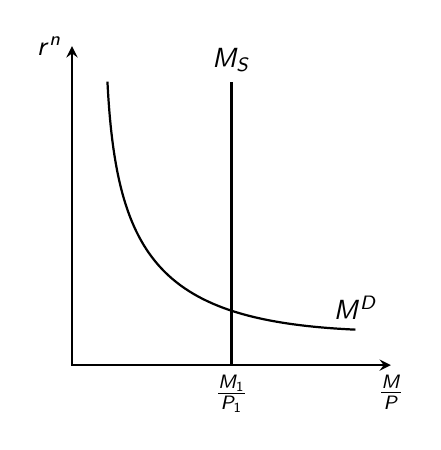
\begin{tikzpicture}[scale=0.45]
			\draw [thick, <->] (0,9) node[left]{\(r^n\)} -- (0,0) -- (9,0) node[below]{\(\frac{M}{P}\)};
			\draw [thick] (1,8) .. controls (1.25,3) and (2.5,1.25) .. (8,1) node [above]{\( M^D \)};
			\draw [thick] (4.5,0) node [below]{\(\frac{M_1}{P_1}\)} -- (4.5,8) node [above]{\( M_S \)};
		\end{tikzpicture}
		\caption{Demand and Supply for money}
	\end{marginfigure}
\subsubsection{Simple Monetary Policy}
	\begin{itemize}
		\item The New Keynesian model suggestions that money affects the real economy
		\item Simple example:
		\begin{itemize}
			\item Assume that \textcolor{myblue}{nominal price rigidities} mean that prices are constant: \( P_1 = P_2 = P \)
			\item Now consider an unexpected increase in money supply \( \uparrow M_1^S \)
			\item What happens to consumption \( (C_1, C_2) \)?
		\end{itemize}
		\item Note: These assumptions only hold in the \textcolor{myblue}{short run!}
		\item With sticky prices (i.e. P constant), an increase in the money supply \textbf{decreases} the nominal interest rate
	\end{itemize}
	\begin{marginfigure}
		\centering
		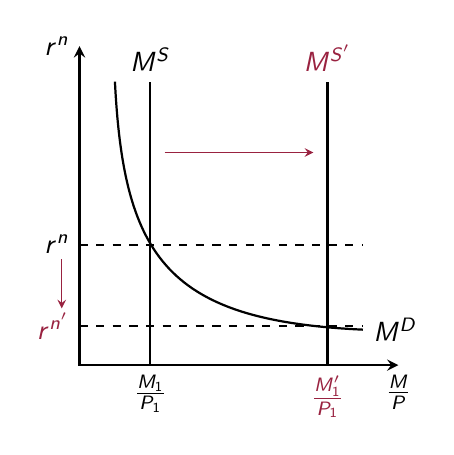
\begin{tikzpicture}[scale=0.45]
			\draw [thick, <->] (0,9) node[left]{\(r^n\)} -- (0,0) -- (9,0) node[below]{\(\frac{M}{P}\)};
			\draw [thick] (1,8) .. controls (1.25,3) and (2.5,1.25) .. (8,1) node [right]{\( M^D \)};
			\draw [thick] (2,0) node [below]{\(\frac{M_1}{P_1}\)} -- (2,8) node [above]{\( M^S \)};
			\draw [->,color=myred] (2.4,6) -- (6.6,6);
			\draw [thick] (7,0) node [below,color=myred]{\(\frac{M_1'}{P_1}\)} -- (7,8) node [above,color=myred]{\( M^{S'} \)};
			\draw [thick,dashed] (0,1.1) node [left,color=myred]{\( r^{n'} \)} -- (8,1.1);
			\draw [<-,color=myred] (-0.5,1.6) -- (-0.5,3);
			\draw [thick,dashed] (0,3.4) node [left]{\( r^n \)} -- (8,3.4);
		\end{tikzpicture}
		\caption{Sticky prices}
	\end{marginfigure}
	\begin{itemize}
		\item To solve for changes in consumption take the inter-temporal budget constraint, money demand, and Euler equations (assuming that \( P_1 = P_2 \)):
		\begin{align*}
			C_1 + \frac{M_1}{P_1} + \frac{C_2}{1 + r^n} &= Y_1 + \frac{Y_2}{1 + r^n} + \frac{M_1 / P_1}{1 + r^n}\\
			\omega \frac{C_1}{M_1 / P_1} &= \left( \frac{r^n}{1 + r^n} \right) \\
			\frac{1}{C_1} &= \beta (1+ r^n) \frac{1}{C_2}
		\end{align*}
		\item Substituting the money demand and Euler equations into the budget constraint, we get the consumption functions:
		\[
			C_1 = \frac{1}{1 + \omega + \beta} \left( Y_1 + \frac{Y_2}{1 + r^n} \right), \quad C_2 = \frac{\beta (1 + r^n)}{1 + \omega + \beta} \left( Y_1 + \frac{Y_2}{1 + r^n} \right)
		\]
		\item Remember the increase in money supply leads to a \textcolor{myblue}{decrease in \( r^n \)}
		\item Thus, consumption in period 1 rises:
		\[
			\textcolor{myblue}{\uparrow C_1} = \frac{1}{1 + \omega + \beta} \left( Y_1 + \frac{Y_2}{\textcolor{myblue}{\underbrace{(1 + r^n)}_\downarrow}} \right), 
		\]
		\item And consumption in period 2 falls:
		\[
			\textcolor{myblue}{\downarrow C_2} = \frac{\beta (1 + r^n)}{1 + \omega + \beta} \left( Y_1 + \frac{Y_2}{1 + r^n} \right) = \frac{\beta \textcolor{myblue}{\overbrace{(1 + r^n)}^\downarrow}}{1 + \omega + \beta} Y_1 + \frac{\beta}{1 + \omega + \beta} Y_2
		\]
		\item So sticky prices mean that \textcolor{myblue}{monetary policy is non-neutral} in the short run
		\begin{itemize}
			\item That is, monetary policy can have \textcolor{myblue}{real effects} on the macroeconomy!
		\end{itemize}
		\item Changes in monetary policy also affect demand for assets!
		\item Derive the bond demand equation using the period 1 budget constraint and the money demand equation:
		\begin{align*}
			\frac{B_2}{P_1} &= Y_1 - C_1 - \frac{M_1}{P_1} \\
			&= Y_1 - C_1 - \omega C_1 \left( 1 + \frac{1}{r^n} \right)
		\end{align*}
		\item Which shows that real bond demand is \textbf{increasing} in the nominal interest rate rn
		\item So households \textcolor{myblue}{adjust their asset portfolio} according to the return on bonds
		\item Changes in monetary policy affect real \textcolor{myblue}{asset portfolio allocation decisions}
		\item Household composition of assets varies with the relative return on the assets available
		\item So a decrease in money supply raises the nominal interest rate, which increases bond holdings
		\item Since the nominal return on money is zero, an increase in the nominal return on bonds leads to a shift away from money and towards bonds
	\end{itemize}
	\begin{marginfigure}
		\centering
		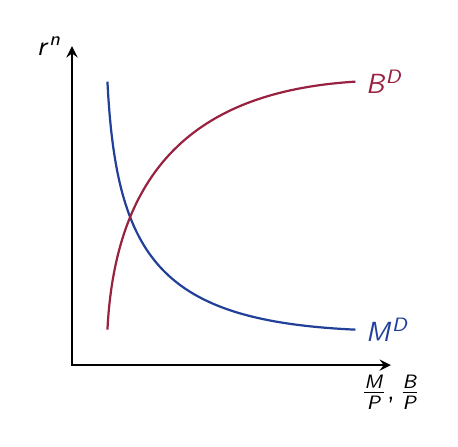
\begin{tikzpicture}[scale=0.45]
			\draw [thick, <->] (0,9) node[left]{\(r^n\)} -- (0,0) -- (9,0) node[below]{\(\frac{M}{P},\frac{B}{P}\)};
			\draw [thick,color=myblue] (1,8) .. controls (1.25,3) and (2.5,1.25) .. (8,1) node [right]{\( M^D \)};
			\draw [thick,color=myred] (1,1) .. controls (1.25,6) and (4,7.75) .. (8,8) node [right]{\( B^D \)};
		\end{tikzpicture}
		\caption{Bond market}
	\end{marginfigure}
\subsection{Limitations of the New Keynesian Model}
	\begin{itemize}
		\item The source of price rigidities is often not well-microfounded
		\begin{itemize}
			\item Typically introduce ad-hoc ``price stickiness'' to models
		\end{itemize}
		\item New Keynesian models often do not account for macroeconomic data much better than RBC models
		\item Despite their basis in monetary economics, New Keynesian models often do a poor job of explaining fluctuations in inflation
		\item As was the case for the RBC model, most New Keynesian models are not solved with \textcolor{myred}{economic risk} in mind
		\item So, again, these models are not ideal for studying some of the main motives for asset holdings
		\item Both RBC and New Keynesian models contain a single, \textcolor{myred}{representative household}
		\item This household has no one else to trade with, so the notion of a financial market is limited
	\end{itemize}
\section{Expectations, Uncertainty, and Asset Holdings}\label{Sec:5}
\subsection{Risk Aversion and the Precautionary Savings Motive}
	\begin{itemize}
		\item \textcolor{myblue}{Risk aversion:} a tendency to prefer economic outcomes with low uncertainty to those with more uncertainty
		\item \textcolor{myblue}{Precautionary Savings:} an increase in income uncertainty that leaves expected income unchanged reduces current consumption. But savings increase as a form of self \textbf{\textcolor{myblue}{insurance}} against low income states of the world.
		\item \textcolor{myblue}{Risk aversion} is a consequence of diminishing marginal utility
		\begin{itemize}
			\item For utility function \( u(\cdot) \), then \( u' > 0 \) and \( u'' < 0 \)
			\item Implies a loss of \( x \) matters more than a gain \( x \)
			\item A risk averse agent would turn down a fair bet with even odds of an increase of \( x \) or a decrease in \( x \)
			\item But risk aversion does not tell us how an agent \textit{responds} to uncertainty or risk
		\end{itemize}
		\item \textcolor{myblue}{Precautionary Savings} is a result of marginal utility declining at a decreasing rate:
		\begin{itemize}
			\item For utility function \( u(\cdot) \), then \( u''' > 0 \)
			\item This feature of utility functions/preferences is sometimes called \textbf{prudence}
		\end{itemize}
		\item In this case, an increase in income uncertainty (holding expected income constant) raises expected \textbf{marginal utility}
		\item This means that the value of \textbf{additional} consumption is higher, which means that households save more in order to consume more in the periods of heightened uncertainty
		\item These additional savings in the face of greater uncertainty are called \textcolor{myblue}{precautionary savings}
	\end{itemize}
\subsection{The Precautionary Savings Motive: An Illustrative Model}
	\begin{itemize}
		\item A household makes consumption and savings decisions, subject to known and constant incomes
		\item Assume \( \beta = 1 \) return on savings is zero \( (r = 0) \), income in each period is \(\overline{Y}\), utility function \( u' > 0, u'' < 0, u''' > 0 \)
		\begin{align*}
			\max_{C_1,C_2}\quad &u(C_1) + u(C_2) \\
			\text{s.t.}\quad &C_1 + C_2 = \overline{Y} + \overline{Y}
		\end{align*}
		\item The first order condition yields the optimality condition (Euler Equation):
		\begin{align*}
			u'(C_1) &= u'(C_2) \\
			\Rightarrow C_1 &= C_2 = \overline{Y}
		\end{align*}
		\item Label these consumption choices \( C_1^c \) and \( C_2^c \) for the choices under \textbf{certainty}
		\item It will be helpful to plot marginal utility as a function of consumption in period 2
		\item First, plot marginal utility at our consumption choice under certainty \( C_2^c \)
		\item Note that because \( u'' < 0 \) and \( u''' > 0 \), marginal utility is decreasing and convex (i.e. curved out from the origin)
	\end{itemize}
	\begin{figure}[H]
		\centering
		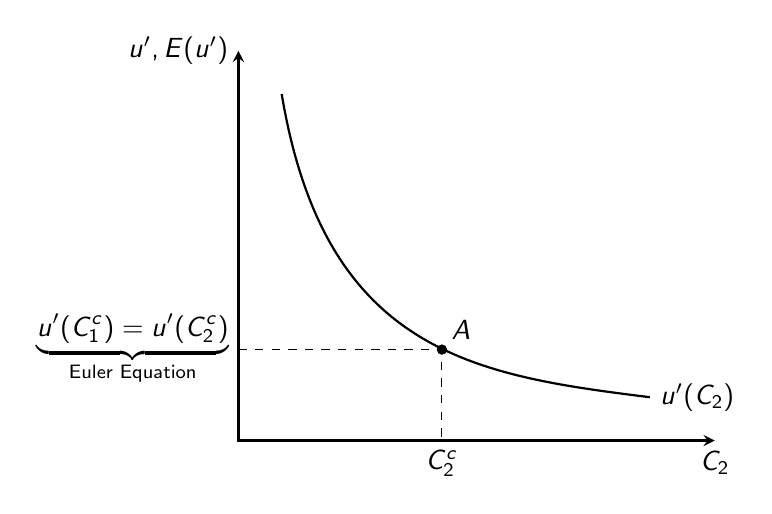
\begin{tikzpicture}[scale=0.55]
			\draw [thick, <->] (0,9) node[left]{\(u',E(u')\)} -- (0,0) -- (11,0) node[below]{\(C_2\)};
			\draw [thick] (1,8) .. controls (2,2) and (5.5,1.5) .. (9.5,1) node [right]{\( u'(C_2) \)};
			\draw [dashed] (0,2.1) node [left]{\( \underbrace{u'(C_1^c) = u'(C_2^c)}_\text{Euler Equation} \)}-- (4.7,2.1) -- (4.7,0) node [below]{\( C_2^c \)};
			\filldraw[black] (4.7,2.1) circle (3pt) node [above right]{\( A \)};
		\end{tikzpicture}
	\end{figure}
	\begin{itemize}
		\item Now suppose there are different \textbf{states} of the world
		\item These states affect income in period 2, with a chance of a good outcome and a chance of a bad outcome
		\[	
			Y_2= 
			\begin{cases}
				\overline{Y} + x & \text{with probability 0.5 \quad (Good Outcome)} \\
				\overline{Y} - x & \text{with probability 0.5 \quad (Bad Outcome)}
			\end{cases}
		\]
		\item The first order condition in this case yields the \textcolor{myblue}{Expected Euler Equation:}
		\[
			u'(C_1) = E(u'(C_2))
		\]
		\item Where \( E(u'(C_2)) \) is the expectation over \textbf{marginal utility} of consumption in period 2
		\item Note that we can compute this as:
		\begin{align*}
			E(u'(C_2)) &= 0.5 \times u'(C_2(good)) + 0.5 \times u'(C_2(bad)) \\
			&= 0.5 \times u'(C_2(\overline{Y} + x + S)) + 0.5 \times u'(C_2(\overline{Y} - x + S))
		\end{align*}
		\item Suppose the household were to choose period 1 consumption the same as under the certainty case: \( C_1 = C_1^c = \overline{Y} \)
		\item Then from the period 1 budget constraint, savings are: \( S = \overline{Y} - C_1^c \)
		\item And we can write consumption in period two as:
		\begin{align*}
			C_2 &= Y_2 + S \\
			&= Y_2 + \overline{Y} - C_1^c \\
			&=
			\begin{cases}
				\overline{Y} + x + \overline{Y} - C_1^c & \text{with probability 0.5} \\
				\overline{Y} - x + \overline{Y} - C_1^c & \text{with probability 0.5}
			\end{cases}
			\\
			&=
			\begin{cases}
				C_2^c + x & \text{with probability 0.5} \\
				C_2^c + x & \text{with probability 0.5}
			\end{cases}
		\end{align*}
		\item If choosing the certainty consumption in period 1, period 2 consumption is equal to the certainty consumption \( (C_2^c) \) plus or minus the uncertain component of income \( x \)
		\item Now, write the expected marginal utility of consumption in period 2 as:
		\begin{align*}
			E(u'(C_2)) &= 0.5 \times u'(C_2^c + x) + 0.5 \times u' (C_2^c - x) \\
			&\geq u'(C_2^c)
		\end{align*}
		\item Because \( u''' > 0 \) the expected marginal utility of consumption in the \textcolor{myblue}{uncertain} case is greater than marginal utility in the \textcolor{myred}{certain} case
		\item This means that the value of the certain consumption choice is greater than the value of the uncertain consumption outcomes
		\item Another way: \textcolor{myblue}{households prefer certainty to uncertainty, even when the expected value of outcomes is the same in both cases}
		\item Again consider plot of marginal utility as function of consumption in period 2
		\item Consumption is low/marginal utility is high in the bad state (1)
		\item Consumption is high/marginal utility is low in the good state (2)
	\end{itemize}
	\begin{figure}[H]
		\centering
		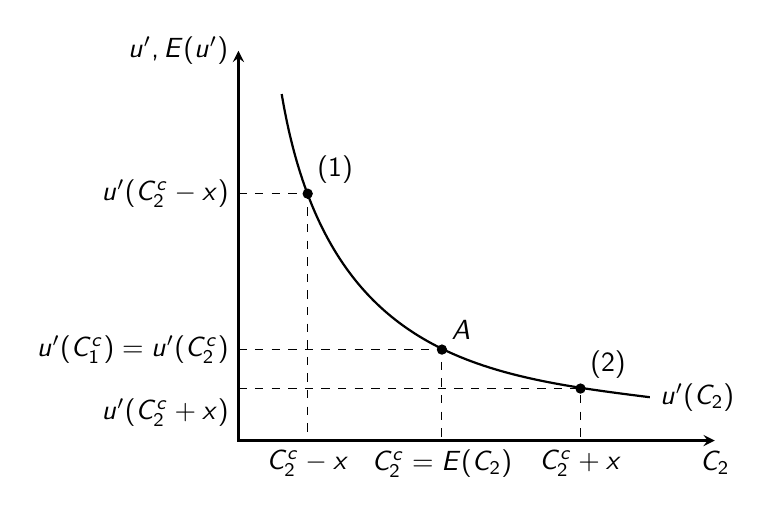
\begin{tikzpicture}[scale=0.55]
			\draw [thick, <->] (0,9) node[left]{\(u',E(u')\)} -- (0,0) -- (11,0) node[below]{\(C_2\)};
			\draw [thick] (1,8) .. controls (2,2) and (5.5,1.5) .. (9.5,1) node [right]{\( u'(C_2) \)};
			\draw [dashed] (0,2.1) node [left]{\( u'(C_1^c) = u'(C_2^c) \)} -- (4.7,2.1) -- (4.7,0) node [below]{\( C_2^c = E(C_2) \)};
			\filldraw[black] (4.7,2.1) circle (3pt) node [above right]{\( A \)};
			\draw [dashed] (0,5.7) node [left]{\( u'(C_2^c - x) \)} -- (1.6,5.7) -- (1.6,0) node [below]{\( C_2^c - x \)};
			\filldraw[black] (1.6,5.7) circle (3pt) node [above right]{\( (1) \)};
			\draw [dashed] (0,1.2) node [below left]{\( u'(C_2^c + x) \)} -- (7.9,1.2) -- (7.9,0) node [below]{\( C_2^c + x \)};
			\filldraw[black] (7.9,1.2) circle (3pt) node [above right]{\( (2) \)};
		\end{tikzpicture}
	\end{figure}
	\begin{itemize}
		\item Notice that: \( E(u'(C_2)) > \underbrace{u'(C_2^c) = u'(C_1^c)}_\text{Euler Equation} \)
		\item Therefore:
		\begin{itemize}
			\item Households want to increase \( C_2 \), and decrease \( C_1 \),
			\item They accomplish this with higher (i.e. precautionary) savings \( S \)
		\end{itemize}
	\end{itemize}
	\begin{figure}[H]
		\centering
		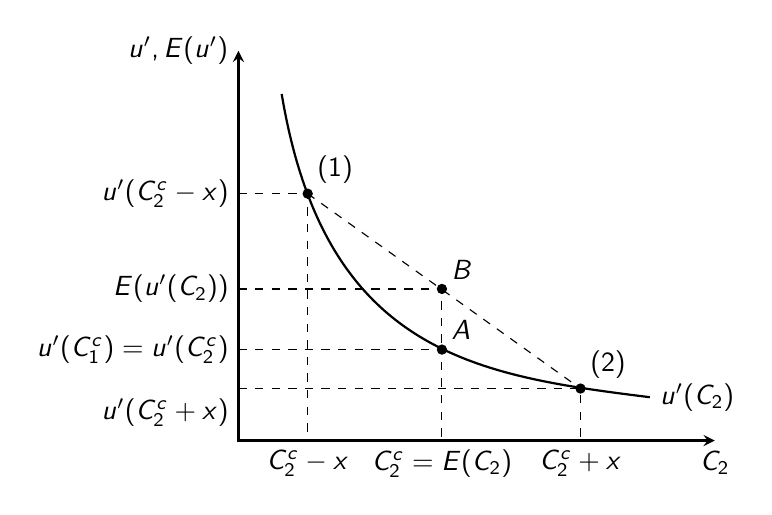
\begin{tikzpicture}[scale=0.55]
			\draw [thick, <->] (0,9) node[left]{\(u',E(u')\)} -- (0,0) -- (11,0) node[below]{\(C_2\)};
			\draw [thick] (1,8) .. controls (2,2) and (5.5,1.5) .. (9.5,1) node [right]{\( u'(C_2) \)};
			\draw [dashed] (0,2.1) node [left]{\( u'(C_1^c) = u'(C_2^c) \)} -- (4.7,2.1) -- (4.7,0) node [below]{\( C_2^c = E(C_2) \)};
			\filldraw[black] (4.7,2.1) circle (3pt) node [above right]{\( A \)};
			\draw [dashed] (0,5.7) node [left]{\( u'(C_2^c - x) \)} -- (1.6,5.7) -- (1.6,0) node [below]{\( C_2^c - x \)};
			\filldraw[black] (1.6,5.7) circle (3pt) node [above right]{\( (1) \)};
			\draw [dashed] (0,1.2) node [below left]{\( u'(C_2^c + x) \)} -- (7.9,1.2) -- (7.9,0) node [below]{\( C_2^c + x \)};
			\filldraw[black] (7.9,1.2) circle (3pt) node [above right]{\( (2) \)};
			\draw [dashed] (1.6,5.7) -- (7.9,1.2);
			\draw [dashed] (0,3.5) node[left]{\( E(u'(C_2)) \)} -- (4.7,3.5)-- (4.7,2.1);
			\filldraw[black] (4.7,3.5) circle (3pt) node [above right]{\( B \)};
		\end{tikzpicture}
	\end{figure}
	\begin{itemize}
		\item Point \textcolor{myblue}{(A)} corresponds to marginal utility of the certain consumption \( C_2^c \)
		\item This is the optimal consumption choice for the certainty case: \( u'(C_1^c) = u'(C_2^c) \)
		\item Point \textcolor{myblue}{(B)} is the \textbf{expected marginal utility} over consumption in the uncertain case: \( E(u'(C_2)) \)
		\item Note that \( E(u'(C_2)) > u'(C_2^c) = u'(C_1^c) \)
		\item This means that consumption is \textbf{too low} in period 2 (i.e. marginal utility is too high)
		\item Therefore, the household should consume less in period 1: \( C_1^u < C_1^c \)
		\item This allows household to save more and so consume more in period 2: \( C_2^u(s) > C_2^c(s) \)
	\end{itemize}
\subsection{Precautionary Savings and Asset Prices}
	\begin{itemize}
		\item Consider our two-period model:
		\begin{align*}
			\max_{C_1,C_2}\quad &u(C_1) + u(C_2) \\
			\text{s.t.}\quad &C_1 + P_b B = \overline{Y} \\
			&\quad C_2 = Y_2 + B
		\end{align*}
		\item Where a one period bond \( B \) can be purchased at price \( P_b \)
		\item Income is again uncertain:
		\[
			Y_2 =
			\begin{cases}
				\overline{Y} + x & \text{with probability 0.5 \quad (Good Outcome)} \\
				\overline{Y} - x & \text{with probability 0.5 \quad (Bad Outcome)}
			\end{cases}
		\]
		\item The first order condition yields the Expected Euler Equation:
		\[
			P_b u'(C_1) = \beta E (u'(C_2))
		\]
		\item And rearranging we have:
		\[
			P_b = \beta \frac{E(u'(C_2))}{u'(C_1)}
		\]
		\item This is referred to as an \textcolor{myblue}{Asset Pricing Equation}
		\item Asset prices determined by the ratio of marginal utilities of consumption in each period
		\item Or, another way: asset prices are given by the marginal rate of substitution between consumption across periods. \textcolor{myblue}{How does uncertainty affect prices?}
		\item So now consider an increase from \( x \) to \( x^* \):
		\begin{itemize}
			\item Now \( Y_2 = \overline{Y} + x^* > \overline{Y} + x \) with probability 0.5, and \( Y_2 = \overline{Y} - x^* < \overline{Y} - x \) with probability 0.5
			\item But it is still the case that \( E(Y_2) = \overline{Y} \)
			\item This is called a \textcolor{myblue}{mean-preserving spread} in \( Y_2 \)
			\item Uncertainty only affects period 2, so the effect on asset prices comes through  \( E(u'(C_2)) \)
		\end{itemize}
	\end{itemize}
	\begin{figure}[H]
		\centering
		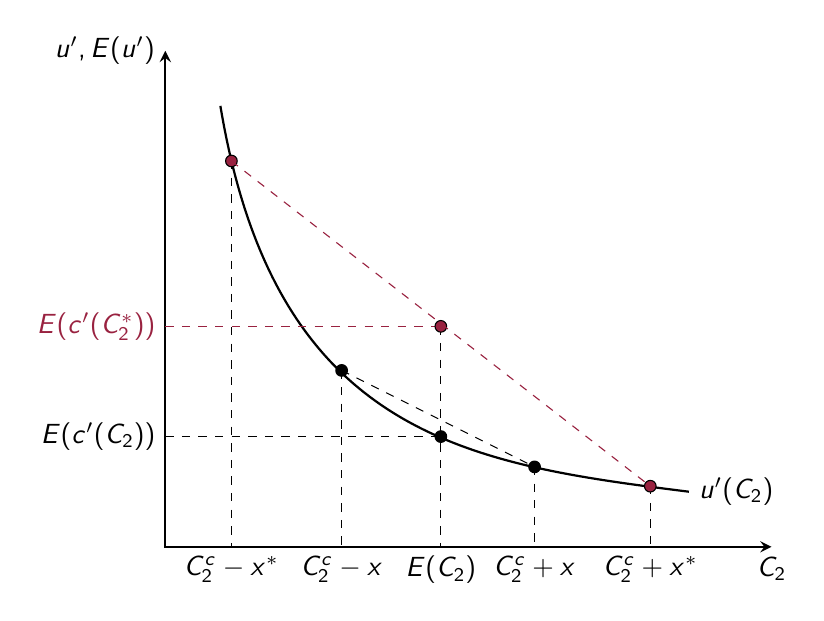
\begin{tikzpicture}[scale=0.7]
			\draw [thick, <->] (0,9) node[left]{\(u',E(u')\)} -- (0,0) -- (11,0) node[below]{\(C_2\)};
			\draw [thick] (1,8) .. controls (2,2) and (5.5,1.5) .. (9.5,1) node [right]{\( u'(C_2) \)};
			\draw [dashed] (0,2) node [left]{\( E(c'(C_2)) \)} -- (5,2) -- (5,0) node [below]{\( E(C_2) \)};
			\filldraw[black] (5,2) circle (3pt);
			\draw[dashed,color=myred] (0,4) node [left]{\( E(c'(C_2^*)) \)} -- (5,4);
			\draw[dashed] (5,4) -- (5,2);
			\filldraw[fill=myred,draw=black] (5,4) circle (3pt);
			\draw [dashed] (1.2,7) -- (1.2,0) node [below]{\( C_2^c - x^* \)};
			\filldraw[fill=myred,draw=black] (1.2,7) circle (3pt);
			\draw [dashed] (8.8,1.1) -- (8.8,0) node [below]{\( C_2^c + x^* \)};
			\filldraw[fill=myred,draw=black] (8.8,1.1) circle (3pt);
			\draw [dashed,color=myred] (1.2,7) -- (8.8,1.1);
			\draw [dashed] (3.2,3.2) -- (3.2,0) node [below]{\( C_2^c - x \)};
			\filldraw[black] (3.2,3.2) circle (3pt);
			\draw [dashed] (6.7,1.45) -- (6.7,0) node [below]{\( C_2^c + x \)};
			\filldraw[black] (6.7,1.45) circle (3pt);
			\draw [dashed] (3.2,3.2) -- (6.7,1.45);
		\end{tikzpicture}
	\end{figure}
	\begin{itemize}
		\item Since \( E(c'(C_2)) \) increases, \( P_b \) increases also:
		\[
			\textcolor{myred}{\uparrow}P_b = \beta \frac{E(u'(C_2))\textcolor{myred}{\uparrow}}{u'(C_1)}
		\]
		\item But \( C_1 \) also decreases in response to greater uncertainty, which increases \( u'(C_1) \)
		\item So what is the overall effect?
		\item Substitute in the budget constraints:
		\[
			P_b = \beta \frac{E(u'(Y_2 + B))}{u'(\overline{Y} - P_b B)}
		\]
		\item Illustrate optimal choices graphically by plotting the left-hand-side and right-hand-side of the asset pricing equation
	\end{itemize}
	\begin{figure}[H]
		\centering
		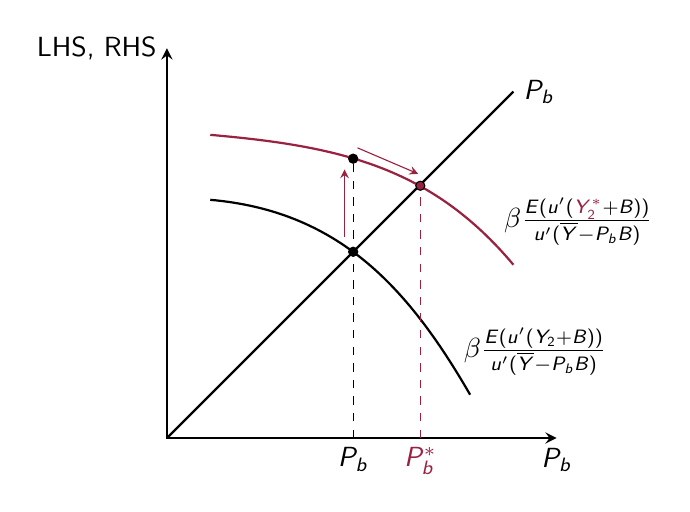
\begin{tikzpicture}[scale=0.55]
			\draw [thick, <->] (0,9) node[left]{LHS, RHS} -- (0,0) -- (9,0) node[below]{\(P_b\)};
			\draw [thick] (0,0) -- (8,8) node [right] {\( P_b \)};
			\draw [thick] (1,5.5) to [in=120,out=-5] (7,1);
			\node at (8.5,2) {\( \beta \frac{E(u'(Y_2 + B))}{u'(\overline{Y} - P_b B)} \)};
			\draw [dashed] (4.3,0) node [below]{\( P_b \)}  -- (4.3,6.45);
			\draw [thick,color=myred] (1,7) to [in=130,out=-5] (8,4);
			\node at (9.5,5) {\( \beta \frac{E(u'(\textcolor{myred}{Y_2^*} + B))}{u'(\overline{Y} - P_b B)} \)};
			\draw [dashed,color=myred] (5.85,0) node [below]{\( P_b^* \)} -- (5.85,5.825);
			\filldraw[fill=myred,draw=black] (5.85,5.825) circle (3pt);
			\filldraw[black] (4.3,6.45) circle (3pt);
			\filldraw[black] (4.3,4.3) circle (3pt);
			\draw [->,color=myred] (4.1,4.65) -- (4.1,6.2);
			\draw [->,color=myred] (4.4,6.7) -- (5.8,6.1);
		\end{tikzpicture}
	\end{figure}
	\begin{itemize}
		\item An increase in uncertainty \textbf{increases} the price of assets
		\item This is intuitive:
		\begin{itemize}
			\item Greater uncertainty induces precautionary savings which increases demand for assets
			\item  Higher asset demand is associated with higher asset 
		\end{itemize}
		\item Recall that the asset return: \( R = \frac{1}{P_b} \)
		\item So higher asset prices are associated with \textbf{lower} asset returns
		\item Do we observe this empirically?
	\end{itemize}
	\begin{figure}[H]
		\centering
		\begin{tikzpicture}
			\begin{axis}[
				no markers,
				axis on top,
				height = \axisdefaultheight,
				width = 0.95\textwidth,
				date coordinates in = x,
				date ZERO = {1990-01-01},
				xticklabel = {\year},
				xtick = {
					1992-01-01,
					1996-01-01,
					2000-01-01,
					2004-01-01,
					2008-01-01,
					2012-01-01,
					2016-01-01,
					2020-01-01
				},
				xmin = 1990-01-01,
				xmax = 2022-07-01,
				xtick pos = left,
				xtick align = outside,
				ytick = {0,2,4,6,8,10},
				ytick pos = bottom,
				ytick align = outside,
				ymin = -1,
				ymax = 11,
				legend pos = north west,
				legend cell align = left,
				legend style = {font=\scriptsize,draw=none,fill opacity=0.75,cells={align=left}},
				legend entries = {{Equity Market Volatility Tracker\\ (Bloom et al., 2019; scaled)}, 3 Month 	Treasury Bond Return},
				]
				\addplot+[color=myblue,thick,smooth] table [x=Date,y=EM,col sep=comma] {Equity-Market.csv};
				\addplot+[color=myred,thick,smooth] table [x=Date,y=3Month,col sep=comma] {Equity-Market.csv};
				\addplot [draw=none,fill=gray,opacity=0.15] coordinates {(1990-07-01, -1) (1990-07-01, 11) (1991-03-01, 11) (1991-03-01, -1)};
				\addplot [draw=none,fill=gray,opacity=0.15] coordinates {(2001-03-01, -1) (2001-03-01, 11) (2001-11-01, 11) (2001-11-01, -1)};
				\addplot [draw=none,fill=gray,opacity=0.15] coordinates {(2007-12-01, -1) (2007-12-01, 11) (2009-06-01, 11) (2009-06-01, -1)};
				\addplot [draw=none,fill=gray,opacity=0.15] coordinates {(2020-02-01, -1) (2020-02-01, 11) (2020-04-01, 11) (2020-04-01, -1)};
			\end{axis}
		\end{tikzpicture}
	\end{figure}
	\begin{itemize}
		\item Note, we need to compare \textcolor{myblue}{risk-free} bonds
		\item For \textcolor{myred}{risky assets}, demand and prices may increase or decrease depending on the nature of the asset risk
	\end{itemize}
	\begin{figure}[H]
		\centering
		\begin{tikzpicture}
			\begin{axis}[
				no markers,
				axis on top,
				height = \axisdefaultheight,
				width = 0.95\textwidth,
				date coordinates in = x,
				date ZERO = {1990-01-01},
				xticklabel = {\year},
				xtick = {
					1992-01-01,
					1996-01-01,
					2000-01-01,
					2004-01-01,
					2008-01-01,
					2012-01-01,
					2016-01-01,
					2020-01-01
				},
				xmin = 1990-01-01,
				xmax = 2022-07-01,
				xtick pos = left,
				xtick align = outside,
				ytick = {0,2,4,6,8,10},
				ytick pos = bottom,
				ytick align = outside,
				ymin = -1,
				ymax = 11,
				legend pos = north west,
				legend cell align = left,
				legend style = {font=\scriptsize,draw=none,fill opacity=0.75,cells={align=left}},
				legend entries = {{Equity Market Volatility Tracker\\ (Bloom et al., 2019; scaled)}, Aaa Corporate Bond Spread\\ Over 10-Year Treasury, Baa Corporate Bond Spread\\ Over 10-Year Treasury}
				]
				\addplot+[color=myblue,thick,smooth] table [x=Date,y=EM,col sep=comma] {Equity-Market.csv};
				\addplot+[color=myred,thick,smooth] table [x=Date,y=Aaa,col sep=comma] {Equity-Market.csv};
				\addplot+[color=mygreen,thick,smooth] table [x=Date,y=Baa,col sep=comma] {Equity-Market.csv};
				\addplot [draw=none,fill=gray,opacity=0.15] coordinates {(1990-07-01, -1) (1990-07-01, 11) (1991-03-01, 11) (1991-03-01, -1)};
				\addplot [draw=none,fill=gray,opacity=0.15] coordinates {(2001-03-01, -1) (2001-03-01, 11) (2001-11-01, 11) (2001-11-01, -1)};
				\addplot [draw=none,fill=gray,opacity=0.15] coordinates {(2007-12-01, -1) (2007-12-01, 11) (2009-06-01, 11) (2009-06-01, -1)};
				\addplot [draw=none,fill=gray,opacity=0.15] coordinates {(2020-02-01, -1) (2020-02-01, 11) (2020-04-01, 11) (2020-04-01, -1)};
			\end{axis}
		\end{tikzpicture}
	\end{figure}
\subsection{How Much Does the Precautionary Savings Motive Matter?}
	\begin{itemize}
		\item The two motives for asset holding that we have studied so far:
		\begin{itemize}
			\item Life-cycle motive: consumption smoothing across time
			\item Precautionary savings motive: consumption smoothing across outcomes/states of the world
		\end{itemize}
		\item Finds that precautionary savings matter much more for young households' asset decisions
		\item Finds that life-cycle motives matter much more for older households' asset decisions
		\item Young households start out with low wealth, need to save to build a \textbf{\textcolor{myblue}{precautionary savings buffer}}
	\end{itemize}
\section[Introduction to Asset Pricing]{Introduction to Asset Pricing: Concepts, Measurement, and a Simple Model}\label{Sec:6}
\subsection{Definitions and Measurement}
	\begin{itemize}
		\item Consider simple asset that was bought last period at \( P_{t-1} \) and sold this period at \( P_t \)
		\item The simple net return \( r_t \) on this asset between dates \( t - 1 \) and \( t \) is:
		\[
			r_t = \frac{P_t - P_{t-1}}{P_{t-1}} = \frac{P_t}{P_{t-1}} - 1
		\]
		\item The simple gross return is: \( R_t = 1 + r_t \)
		\item The gross return on the asset over \( k \) periods starting at date \( t - k \) is:
		\begin{align*}
			R_t(k) &= R_t \cdot R_{t-1} \cdots R_{t-k+1}\\
			&= \frac{P_t}{P_{t-1}} \cdot \frac{P_{t-1}}{P_{t-2}} \cdots \frac{P_{t-k+1}}{P_{t-k}} \\
			&= \frac{P_t}{P_{t-k}}
		\end{align*}
		\item These multi-period returns are referred to as \textbf{compounded returns}
		\item Multi-year returns are often annualised in order to easily compare investments in assets over different horizons
		\item An annualised gross return \( R_t^{ann} (k) \)  is computed via:
		\[
			R_t^{ann} (k) = \left[R_t \cdot R_{t-1} \cdots R_{t-k+1}\right]^{\frac{1}{k}} = \Biggl[\prod_{j=0}^{k-1} R_{t-j}\Biggr]^{\frac{1}{k}}
		\]
		\item This formula is known as a \textbf{geometric mean}
		\item For quick comparisons -- that are less accurate! -- we sometimes use an arithmetic mean as an approximation to the annualised return:
		\[
			R_t^{ann} (k) \approx \frac{1}{k} \sum_{k-1}^{j=0} R_{t-j}
		\]
	\end{itemize}
\subsubsection{Continuous Compounding}
	\begin{itemize}
		\item The continuously compounded return or log-return of an asset is defined as:
		\[
			\tilde{r}_t = \log(R_t) = \log \left( \frac{P_t}{P_{t-1}} \right) = \log(P_t) - \log(P_{t-1}) = p_t - p_{t-1}
		\]
		\item where lower-case letters represent the log of a variable
		\item So the continuously compounded multi-period return over k periods is:
		\begin{align*}
			\tilde{r} &= \log(R_t(k))\\
			&= \log(R_t) + \log(R_{t-1}) + \cdots + \log(R_{t-k+1})\\
			&= \tilde{r} + \tilde{r}_{t-1} + \cdots + \tilde{r}_{t-k+1}
		\end{align*}
		\item Compounding -- a multiplicative operation -- is converted to an additive operation by taking logarithms!
	\end{itemize}
\subsubsection{Dividend payments}
	\begin{itemize}
		\item Some assets (e.g. stocks) pay out dividends, which make up part of the return on the asset
		\item For these assets, define returns as:
		\begin{align*}
				R_t &= \frac{P_t + D_t}{P_{t-1}} \\
				\Rightarrow r_t &= \frac{P_t + D_t}{P_{t-1}} -1
		\end{align*}
		\item To compute the log-return:
		\[
			\tilde{r}_t = \log(R_t) = \log \left(\frac{P_t + D_t}{P_{t-1}}\right) = \log(P_t+D_t) - \log(P_{t-1})
		\]
	\end{itemize}
\subsubsection{Excess Returns}
	\begin{itemize}
		\item We will often want to compare returns across different assets
		\item Consider the gross return on a benchmark asset \( R_t \)
		\item And consider the gross return \( R_t^i \) on a comparison asset \( i \)
		\item The \textbf{excess return} of asset \( i \) over the benchmark is:
		\[
			R_t^i - R_t = r_t^i - r_t
		\]
		\item In many cases, the benchmark asset will be something approximating a riskless/risk-free asset such as a government bond
	\end{itemize}
\subsubsection{Equity Premium}
	\begin{itemize}
		\item The equity premium is the expected excess return of an asset over the risk-free rate:
		\[
			E_t(R_t^i - R_t)
		\]
		\item The equity premium tells us the excess return on asset \( i \) required to compensate investors for the additional risk of holding \( i \) over the risk-free asset
	\end{itemize}
\subsubsection{Present Value with Constant Discount Rates}
	\begin{itemize}
		\item Suppose an asset paying a regular dividend has a constant expected return \( R_t = R \):
		\[
			R = E_t \left(\frac{P_{t+1} + D_{t+1}}{P_t}\right)
		\]
		\item Rearrange for \( P_t \):
		\begin{equation}
			P_t = E_t \left(\frac{P_{t+1} + D_{t+1}}{R}\right) \label{E:6.1}
		\end{equation}
		\item Note that this is the same as \textcolor{myblue}{the Discounted Cash Flow} valuation model from \cref{Sec:1}
		\item Now step the price forward one period to Pt+1:
		\begin{equation}
				P_{t+1} = E_t \left(\frac{P_{t+2} + D_{t+2}}{R}\right) \label{E:6.2}
		\end{equation}
		\item Substitute back into \cref{E:6.1}:
		\[
			P_t = E_t \left(E_{t+1}\left[\frac{P_{t+2} + D_{t+2}}{R^2}\right]+\frac{D_{t+1}}{R}\right) 
		\]
		\item We can simplify this as:
		\[
			P_t = E_t \left( \frac{P_{t+2} + D_{t+2}}{R^2} + \frac{D_{t+1}}{R}\right) 
		\]
		\item Where the second equality follows from the \textcolor{myblue}{Law of Iterated Expectations} e.g.: \( E_t(E_{t+h}[x_{t+h+1}]) = E_t(x_{t+h+1})\)
		\item Iterating this process K times yields:
		\[
			P_t = E_t \left(\sum_{k=1}^{K}\frac{D_{t+k}}{R^k}\right) + E_t \left(\frac{P_{t+k}}{R^k}\right)
		\]
		\item We typically assume that:
		\[
			\lim_{K\rightarrow\infty} E_t\left(\frac{P_{t+k}}{R^k}\right) = 0
		\]
		\item Which is referred to as the \textcolor{myblue}{No Bubble Condition}
		\item Then we have a simple asset valuation formula:
		\[
			P_t = E_t \left(\sum_{k=1}^{K}\frac{D_{t+k}}{R^k}\right)
		\]
		\item Where the RHS is the discounted present value of future dividends (i.e. cashflows)
	\end{itemize}
\subsection{Introduction to Macroeconomic Models of Asset Pricing}
	\begin{itemize}
		\item How do asset prices relate to the macroeconomic model we have been studying so far?
		\item We will show how the standard model of household behaviour can lead us to a theory of asset pricing known as the \textcolor{myblue}{Consumption Capital Asset Pricing Model} (C-CAPM)
		\item We will then put C-CAPM into the context of the broader study of finance and macro-finance
		\item Consider a household problem at some generic date ``\( t \)''
		\item Two assets:
		\begin{itemize}
			\item A \textcolor{myred}{risk-free bond} \( B_t \). Price \( P_{B,t} \). At \( t+1 \), pays a face value of 1.
			\item A \textcolor{myblue}{risky asset} \( A_t \). Price \( P_{A,t} \) At \( t+1 \), pays uncertain dividend \( D_{t+1} \), and can be resold at price \( P_{A,t+1} \)
		\end{itemize}
		\item The household problem is:
		\begin{align*}
			\max_{C_t,C_{t+1},B_t,A_t}\quad &u(C_t) + \beta E_t[u(C_{t+1})] \\
			\text{s.t.}\quad &C_t + P_{B,t}B_t + P_{A,t}A_t = Y_t \\
			& C_{t+1} = Y_{t+1} + B_t + D_{t+1}A_t + P_{A,t+1}A_t
		\end{align*}
		\item Household chooses \( C_t, B_t, A_t \) at time \( t \), but chooses \( C_{t+1} \) at time \( t+1 \)
		\item But choice of \( B_t, A_t \) affects the budget constraint at time \( t+1 \) where outcomes are uncertain
		\item This uncertainty means the household must form expectations \( (E_t) \) about \( t+1 \) sing information available at time \( t \)
		\item {\large\textcolor{myred}{Important:}}
		\begin{itemize}
			\item Expectations over \( t+1 \) matter for decisions at \( t \) if those decisions affect outcomes at \( t+1 \)!
		\end{itemize}
		\item The Lagrangian Problem is:
		\begin{align*}
			\mathcal{L} &= u(C_t) + \beta E_t[u(C_{t+1})]\\ 
			&+ \lambda_t (Y_t - C_t + P_{B,t}B_t + P_{A,t}A_t)\\ 
			&+ E_t [\lambda_{t+1}(Y_{t+1} + B_t + D_{t+1}A_t + P_{A,t+1}A_t - C_{t+1})]
		\end{align*}
		\item The \textcolor{myblue}{Lagrange Multipliers} \(\lambda_t,\lambda_{t+1}\) measure the shadow value of the budget constraints:
		\begin{itemize}
			\item \( \lambda_t = \) the marginal value of an extra dollar allocated to the budget constraint in period \( t \)
			\item \( \lambda_{t+1} = \) the marginal value of an extra dollar allocated to the budget constraint in period \( t+1 \)
		\end{itemize}
		\item The first order conditions with respect to \( C_t, B_t, A_t \) are:
		\begin{align*}
			C_t:\quad &u'(C_t)-\lambda_t = 0\\
			B_t:\quad &-\lambda_t P_{B,t}+E_t(\lambda_{t+1})=0\\
			A_t:\quad &-\lambda_{t+1} P_{A,t} + E_t(\lambda_{t+1}[D_{t+1}+P_{A,t+1}]) = 0
		\end{align*}
		\item Where expectations enter the FOCs for \( B_t \) and \( A_t \) because those decisions affect outcomes during the uncertain period \( t+1 \)
		\item The first order condition with respect to \( C_{t+1} \) is:
		\[
			C_{t+1}:\quad \beta u'(C_{t+1}) - \lambda_{t+1} = 0
		\]
		\item Where there are \textbf{no expectations} because the decision \( C_{t+1} \) is made \textbf{after} the uncertainty in period \( t+1 \) has been resolved
		\item Tidying up the first order conditions:
		\begin{alignat}{2}
			C_t:\quad &&\lambda_t &= u'(C_t) \label{E:6.3}\\
			C_t+1:\quad &&\lambda_{t+1} &= \beta u'(C_{t+1}) \label{E:6.4}\\
			B_t:\quad &&\lambda_t P_{B,t} &= E_t(\lambda_{t+1}) \label{E:6.5}\\
			A_t:\quad &&\lambda_{t+1} P_{A,t} &= E_t(\lambda_{t+1}[D_{t+1}+P_{A,t+1}]) \label{E:6.6}
		\end{alignat}
	\end{itemize}
\subsubsection{The Macroeconomic Perspective on Asset Prices}
	\begin{itemize}
		\item Combining equations (\ref{E:6.3}), (\ref{E:6.4}) and (\ref{E:6.5}):
		\begin{align*}
			u'(C_t)P_{B,t} &= \beta E_t(u'(C_{t+1}))\\
			\Rightarrow \frac{u'(C_t)}{E_t(u'(C_{t+1}))} &= \frac{1}{P_{B,t}} = R_{B,t}
		\end{align*}
		\item Where the LHS represents the inter-temporal marginal rate of substitution
		\item And \( R_{B,t} \) on the RHS is the (certain) return on the bond
		\item This says that:
		\begin{itemize}
			\item The relative value of consumption across periods is tied to the interest rate (return) on bonds
			\item Or, consumption growth across periods tied to price of transferring resources across periods
		\end{itemize}
		\item \textcolor{myblue}{Macroeconomic Perspective}: inter-temporal consumption is all about interest rates
	\end{itemize}
\subsubsection{The Finance Perspective on Asset Prices}
	\begin{itemize}
		\item Combining equations (\ref{E:6.5}) and (\ref{E:6.6}):
		\begin{alignat*}{2}
			P_{B,t} &= E_t(\frac{\lambda_{t+1}}{\lambda_t}), &&\text{With t+1 payoff = 1}\\
			P_{A,t} &= E_t\left(\frac{\lambda_{t+1}}{\lambda_t}[D_{t+1}+P_{A,t+1}]\right), &\quad&\text{With t+1 payoff = }D_{t+1}+P_{A,t+1} 
		\end{alignat*}
		\item These are known as \textcolor{myblue}{asset pricing equations}
		\item They state that the price of an asset is determined by the valuation of that asset's payoffs
		\item And those valuations are given by the Lagrange Multipliers:
		\begin{itemize}
			\item \( \lambda_t = \) the marginal value of an extra dollar allocated to the budget constraint in period \( t \)
			\item \( \lambda_{t+1} = \) the marginal value of an extra dollar allocated to the budget constraint in period \( t + 1 \)
		\end{itemize}
		\item Looking closely, we can see that both assets' payoffs are valued at the same rate
		\item This valuation is given by the \textcolor{myblue}{stochastic discount factor} (SDF):
		\[
			\frac{\lambda_{t+1}}{\lambda_t}
		\]
		\item For our particular model, we know that the SDF is given by:
		\[
			\frac{\lambda_{t+1}}{\lambda_t} = \beta\frac{u'(C_{t+1})}{u'(C_t)}
		\]
		\item That is, assets are valued by variations in household consumption across time
		\item Since consumption is determined by developments in the macroeconomy: \textcolor{myblue}{asset prices must be linked to business cycle fluctuations!}
		\item Our asset pricing equations are:
		\[
			P_{B,t} = E_t\left(\beta\frac{u'(C_{t+1})}{u'(C_t)}\right), \quad P_{A,t}=E_t\left(\beta\frac{u'(C_{t+1})}{u'(C_t)}[D_{t+1}+P_{A,t+1}]\right) 
		\]
		\item Holding all else equal, asset prices are higher when:
		\begin{itemize}
			\item The marginal utility of current consumption \( C_t \) is low (i.e. \( C_t \) is high)
			\item The marginal utility of current consumption \( C_{t+1} \) is high (i.e. \( C_{t+1} \) is low)
		\end{itemize}
		\item However, it will rarely be the case that \( C_t \) or \( C_{t+1} \) move independent of everything else
		\item Remember, macroeconomic and financial variables move together in equilibrium
		\item Example:
		\begin{itemize}
			\item Consider shares in a firm A that trade at price \( P_{A,t} \) and pay dividends \( D_{t+1} \)
			\item Dividends are paid out of firm profits
			\item Future profits and dividends will be low during recessions
			\item But recessions are times when future consumption is also likely to be low 
		\end{itemize}
		\[
			E_t\left(\beta\frac{\overbrace{u'(C_{t+1})}^{\textcolor{myblue}{\uparrow}}}{u'(C_t)}[\overbrace{D_{t+1}}^{\textcolor{myred}{\downarrow}} + P_{A,t+1}]\right) = P_{A,t} (?)
		\]
		\item So \textcolor{myblue}{risky asset} prices depend on \textcolor{myblue}{co-movement} between future consumption and uncertain payoffs
		\item However, the price of \textcolor{myred}{risk-free assets} (i.e. bonds) only depends on the \textcolor{myred}{SDF}
		\item Previous example: future recession decreases future consumption and dividends
		\[
			P_{B,t}\textcolor{myblue}{\uparrow} = E_t\left(\beta\frac{\overbrace{u'(C_{t+1})}^{\textcolor{myblue}{\uparrow}}}{u'(C_t)}\right), \quad P_{A,t}\textcolor{myred}{\downarrow} = E_t \left(\beta\frac{\overbrace{u'(C_{t+1})}^{\textcolor{myblue}{\uparrow}}}{u'(C_t)}[\overbrace{D_{t+1}}^{\textcolor{myred}{\downarrow\downarrow}} + P_{A,t+1}]\right)
		\]
		\item Which means that the price (return) of \textcolor{myred}{risk-free assets} can move in opposite directions to the prices (returns) of \textcolor{myblue}{risky assets}
	\end{itemize}
	\begin{figure}
		\begin{tikzpicture}[baseline]
			\begin{axis}[
				title = {Various Asset Returns},
				axis on top,
				no markers,
				date coordinates in = x,
				date ZERO = {1986-01-01},
				xticklabel = {\year},
				xtick = {
					1990-01-01,
					2000-01-01,
					2010-01-01,
					2020-01-01
				},
				xmin = 1986-01-01,
				xmax = 2022-08-01,
				ylabel = {Return (\%)},
				ylabel style = {overlay},
				xtick pos = left,
				xtick align = outside,
				ytick = {0.0,2.5,5.0,7.5,10.0,12.5,15.0,17.5},
				ytick pos = bottom,
				ytick align = outside,
				ymin = -1,
				ymax = 18,
				legend pos = north east,
				legend cell align = left,
				legend style = {font=\scriptsize,draw=none,fill opacity=0.75,cells={align=left}},
				legend entries = {3-Year Constant Maturity Government Bond Rate, Moodys Aaa Coporate Bond Yield, Moodys Baa Coporate Bond Yield},
				]
				\addplot+[color=myblue,thick,smooth] table [x=Date,y=DGS3,col sep=comma] {Asset-Returns.csv};
				\addplot+[color=myred,thick,smooth] table [x=Date,y=AAA,col sep=comma] {Asset-Returns.csv};
				\addplot+[color=mygreen,thick,smooth] table [x=Date,y=BAA,col sep=comma] {Asset-Returns.csv};
				\addplot [draw=none,fill=gray,opacity=0.15] coordinates {(1990-07-01, -1) (1990-07-01, 18) (1991-03-01, 18) (1991-03-01, -1)};
				\addplot [draw=none,fill=gray,opacity=0.15] coordinates {(2001-03-01, -1) (2001-03-01, 18) (2001-11-01, 18) (2001-11-01, -1)};
				\addplot [draw=none,fill=gray,opacity=0.15] coordinates {(2007-12-01, -1) (2007-12-01, 18) (2009-06-01, 18) (2009-06-01, -1)};
				\addplot [draw=none,fill=gray,opacity=0.15] coordinates {(2020-02-01, -1) (2020-02-01, 18) (2020-04-01, 18) (2020-04-01, -1)};
			\end{axis}
		\end{tikzpicture}
		\begin{tikzpicture}[baseline]
			\begin{axis}[
				title = {Various Asset Spreads},
				axis on top,
				no markers,
				date coordinates in = x,
				date ZERO = {1986-01-01},
				xticklabel = {\year},
				xtick = {
					1990-01-01,
					2000-01-01,
					2010-01-01,
					2020-01-01
				},
				xmin = 1986-01-01,
				xmax = 2022-08-01,
				ylabel = {Spread (\%)},
				xtick pos = left,
				xtick align = outside,
				ytick = {0,2,4,6,8},
				ytick pos = bottom,
				ytick align = outside,
				ymin = -1,
				ymax = 9,
				legend pos = north west,
				legend cell align = left,
				legend style = {font=\scriptsize,draw=none,fill opacity=0.75,cells={align=left}},
				legend entries = {Spread: Aaa - 3 Year Treasury,Spread: Baa - 3 Year Treasury},
				]
				\addplot+[color=myred,thick,smooth] table [x=Date,y=AAA-DGS3,col sep=comma] {Asset-Spreads.csv};
				\addplot+[color=mygreen,thick,smooth] table [x=Date,y=BAA-DGS3,col sep=comma] {Asset-Spreads.csv};
				\addplot [draw=none,fill=gray,opacity=0.15] coordinates {(1990-07-01, -1) (1990-07-01, 9) (1991-03-01, 9) (1991-03-01, -1)};
				\addplot [draw=none,fill=gray,opacity=0.15] coordinates {(2001-03-01, -1) (2001-03-01, 9) (2001-11-01, 9) (2001-11-01, -1)};
				\addplot [draw=none,fill=gray,opacity=0.15] coordinates {(2007-12-01, -1) (2007-12-01, 9) (2009-06-01, 9) (2009-06-01, -1)};
				\addplot [draw=none,fill=gray,opacity=0.15] coordinates {(2020-02-01, -1) (2020-02-01, 9) (2020-04-01, 9) (2020-04-01, -1)};
			\end{axis}
		\end{tikzpicture}
	\end{figure}
\section{Asset Prices, Consumption, and the Business Cycle}\label{Sec:7}
\subsection{Historical Overview of Finance and Asset Pricing}
	\begin{enumerate}[label=\textbf{\arabic*.}]
		\item \textbf{Market Efficiency View:}
		\begin{itemize}
			\item Asks ``Are market asset prices set conditional on all available information?''
			\item Or ``Can you beat the market return without taking on more than market risk?''
			\item The \\textcolor{myblue}{Efficient Markets Hypothesis:}
			\begin{itemize}
				\item \small [An] old economist and younger economist [are] walking down the street, and the younger economist says, `Look, there's a hundred-dollar bill,' and the older one says, `Nonsense, if it was there somebody would have picked it up already.'
			\end{itemize}
		\end{itemize}
		\item \textbf{Portfolio Theory:}
		\begin{itemize}
			\item How should we form asset portfolios? (Markowitz, 1952)
			\item The variance of the return on an asset portfolio is much smaller than the average of the variances of the returns on the individual assets in the portfolio
			\item So what is the optimal variance of an asset portfolio?
			\item Something called the \textcolor{myblue}{Mean-Variance Efficient Frontier} can be constructed for a portfolio
		\end{itemize}
		\item \textbf{Capital Asset Pricing Model (CAPM):}
		\begin{itemize}
			\item How much do individual asset prices move with the market? (Sharpe 1964; Litner 1965)
			\item Want a model of the cross-sectional behaviour of stock returns
			\item Let \( R_m \) be the return on the ``market'', \( R_f \) is the risk free return, and \( R_i \) is the return on asset \( i \)
			\item Then the excess return on asset \( i \) is:
			\[
				R_i - R_f = \beta_i(R_m - R_f), \:\text{where}\: \beta_i = \frac{\text{Cov}(R_i,R_m)}{\text{Var}(R_m)}
			\]
			\item And \( \beta_i \) can be estimated with regression models (e.g. OLS)
			\item \( \beta_i \) measures an asset's systematic risk/exposure to market fluctuations
			\item Assets with high `betas' are more sensitive to the market
			\item Since investors seek excess returns, this systematic risk is rewarded with higher prices
			\item However, the model does not account for idiosyncratic risk
			\item And while the model does well with cross-sectional data, it performs poorly with time-series data!
		\end{itemize}
		\item \textbf{No-Arbitrage Multi-Risk Theory:}
		\begin{itemize}
			\item No-arbitrage relationships are the key intuition behind modern asset pricing developments
			\item Arbitrage Pricing Theory (APT) is due to Ross, Sharpe, and Merton
			\item Presents a multi-factor approach to asset pricing
			\item This generalizes to multiple sources of risk including: inflation risk, business cycle risk, interest rate risk, exchange rate risk, and default risk.
			\item Multiple `betas' and multiple regression models required.
			\item But the model assumes that \textcolor{myred}{risk} and \textcolor{myred}{risk premiums} are constant
		\end{itemize}
		\item \textbf{Market Microstructure:}
		\begin{itemize}
			\item Studies how the market itself works
			\item E.g. the role of information asymmetry, information trading, market networks, liquidity, trading volume, who is a buyer vs. who is a seller, bid-ask spreads, etc.
		\end{itemize}
		\item \textbf{Macro-Finance Models:}
		\begin{itemize}
			\item C-CAPM (Consumption based CAPM) emerged in the 1980s
			\item Shows how individual attitudes to risk and uncertainty are related to variations in asset prices
			\item The inter-temporal macroeconomic model based on consumer utility functions is central.
			\item The key concept is the \textcolor{myblue}{Stochastic Discount Factor}, otherwise called the \textcolor{myblue}{Pricing Kernel}
			\item In macroeconomic models the SDF is tied to the marginal rate of substitution between consumption across periods
			\item Consumption, which depends on income and wealth, provides the link between business cycles and asset prices in this model
		\end{itemize}
	\end{enumerate}
\subsection{Finance of CAPM}
	\begin{itemize}
		\item The CAPM can be expressed as:
		\[
			R_i - R_f = \beta_i(R_m - R_f)
		\]
		\item where \( r_i \) is return on asset \( i, r_f \) is the risk-free rate, and \( r_m \) is the market portfolio return
		\item The LHS is the excess return on asset \( i \) over the risk-free rate
		\item And the RHS is the excess return on the market portfolio over the risk free rate
		\item The parameter \( \beta_{i,m} \) captures the \textcolor{myblue}{covariance} between the risky asset and the market
		portfolio (scaled by the variance of the market):
		\[
			\beta_{i,m} = \frac{\text{Cov}(R_i,R_m)}{\text{Var}(R_m)}
		\]
		\item Notice that beta is the same as the OLS regression slope coefficient between returns for asset \( i \) and the market \( m \)
		\item The risk of an asset \( i \) is characterised by its covariance with the market portfolio
		\item This particular risk is called \textcolor{myblue}{systematic risk}, and cannot be diversified away
		\begin{itemize}
			\item Why not? Market risk is embedded in all assets, so not possible for any investors to ``take the other side'' of the market
		\end{itemize}
		\item For this reason, systematic risk needs to be rewarded with higher returns
	\end{itemize}
\subsubsection{Understanding the CAPM}
	\begin{itemize}
		\item If the CAPM is thought of like a regression equation, it can be written as:
		\[
			r_i - r_f = \alpha_i +\beta_{i,m} (r_m - r_f) + \varepsilon_i
		\]
		\item where \( \alpha_i \) is the regression intercept/mean excess return
		\item And \( \varepsilon_i \) is the error term/idiosyncratic asset risk
		\item Our standard regression assumptions require:
		\begin{align*}
			E(\varepsilon_i) &= 0\\
			\text{Cov}(r_m,\varepsilon_i) &= 0
		\end{align*}
	\end{itemize}
	\begin{enumerate}[label=\textbf{\arabic*.}]
		\item \textbf{'Alpha'}
		\begin{itemize}
			\item CAPM (but not necessarily the regression formula) predicts that `alpha' should be zero for all assets
			\item This is because the CAPM states that market risk is the only factor driving excess returns
			\item In a regression specification, alpha measures an asset's excess return over and above its risk-adjusted reward
			\item From outside the CAPM perspective, alpha may be picking up other (i.e. non-market) risks that are not captured by the model
		\end{itemize}
		\item \textbf{'Beta'}
		\begin{itemize}
			\item Beta measures an asset's systematic risk
			\item Assets with high betas are more sensitive to the market
		\end{itemize}
		\item \textbf{'Sigma'}
		\begin{itemize}
			\item Sigma measures the (variance) of non-systematic risk
			\item Non-systematic risk is uncorrelated with systematic risk
			\item Often refer to this as idiosyncratic risk
		\end{itemize}
	\end{enumerate}
	\begin{itemize}
		\item Total risk of an asset is decomposed as follows:
		\[
			r_i - r_f = \overbrace{\beta_{i,m}(r_m-r_f)}^\text{Systematic Component} + \overbrace{\varepsilon_i}^\text{Idiosyncratic Component}
		\]
		\item Taking the variance of both sides of the equation:
		\[
			\overbrace{\text{Var}(r_i - r_f)}^\text{Total Risk}= \overbrace{\beta_{i,m}\text{Var}(r_m-r_f)}^\text{Systematic Risk} + \overbrace{\text{Var}(\varepsilon_i)}^\text{Idiosyncratic Risk}
		\]
		\item Note: \( \text{Var}(r_i - r_f) = \text{Var}(r_i) \) and \( \text{Var}(r_m - r_f) = \text{Var}(r_m) \)
		\item CAPM is attractive because:
		\begin{itemize}
			\item It is east to understand and sensible as it is built on modern portfolio theory
			\item It distinguishes between systematic and non-systematic risk
			\item It is very east to implement empirically
		\end{itemize}
	\end{itemize}
\subsubsection{Limitations of CAPM}
	\begin{itemize}
		\item Empirical evidence on the performance of CAPM is mixed
		\item The model does not work well with time series data
		\item This is because in CAPM investors follow myopic strategies as the investment horizon is short and investment opportunities are assumed to be constant over time
		\item But in general there are \textbf{two} types of systematic risks:
		\begin{itemize}
			\item Static (temporal) - Market Risk
			\item Dynamic (inter-temporal) - Changes in investment opportunities
		\end{itemize}
	\end{itemize}
\subsubsection{Multi-Factor CAPM}
	\begin{itemize}
		\item Many papers attempted to build on/improve the simple CAPM model by adding more ``factors''
		\item This literature pioneered by Eugene Fama (Nobel Prize winner) and Kenneth French
		\item Try to identify other explanations for variation in excess returns on a given asset
		\item Find portfolios of traded securities that are highly correlated with different ``factors''
		\item Hypothesize that the risk premium is linearly related to the risk premium on these portfolios:
		\[
			r_i-r_f=\alpha_i+\beta_{i,1}(r_{F1}-r_f)+\beta_{i,2}(r_{F2}-r_f)+\cdots+\beta_{i,K}(r_{FK}-r_f)
		\]
		\item Where \( r_{FK} \) is the return on a portfolio correlated with the \textit{k}-th factor only
		\item Factors might include: firm size, firm leverage, recent firm performance, etc
		\item Multiple regression used to estimate the factor betas
	\end{itemize}
\subsubsection{Limitations of Multi-Factor CAPM}
	\begin{itemize}
		\item May not identify macroeconomic variables that constitute inter-temporal risks
		\item May not specify the relative importance of these inter-temporal risks
		\item Need to identify different sources of inter-temporal risks in asset returns and specifiy relative importance to investors
		\item But the CAPM theory itself gives little guidance on what these factors should be
		\item There are now hundreds (thousands?!) of proposed factors!
		\item This leads to the need for ‘cleaning up’ papers like \textit{Taming the Factor Zoo: A Test of New Factors} by Feng, Giglio, Xiu (2020)
	\end{itemize}
\subsection{Macroeconomics of C-CAPM}
\subsubsection{C-CAPM Model Enviroment}
	\begin{itemize}
		\item We now derive the macro-finance model known as the \textcolor{myblue}{Consumption-CAPM}
		\item This model states that asset prices must be closely related to fluctuations in consumption
		\item The reason being that fluctuations in consumption across time determine willingness to save and take risks
		\item The setup of the model closely follows the model of precautionary savings we studied in \cref{Sec:5}
		\item \( x_{t+1} \) is a random variable
		\item Uncertainty in \( x_{t+1} \) is due to randomness of the \textbf{state} that occurs tomorrow
		\item How do we price or value an asset sold today with this payoff structure?
		\item To know how to value the asset, we need to know an investor's preferences
		\item Consider an investor who maximizes expected inter-temporal utility defined over two periods:
		\[
			u(c_t) + \beta E_t [u(c_{t+1})]
		\]
		\item Where \( \beta \) is the rate at which future utility is discounted (\textbf{not} the CAPM beta!)
		\item \( u(\cdot) \) is a general utility function defined over consumption
		\item And \( E_t \) is the expectations function taken with respect to information available at time \(t\)
	\end{itemize}
\subsubsection{Utility Functions}
	\begin{itemize}
		\item The utility function captures the investor's attitude towards risk
		\item Note that the \textbf{level} of \( u(C) \) does not matter
		\item Instead, it is \textbf{\textcolor{myblue}{marginal utility}} that matters
		\item Marginal utility measures `hunger' rather than `happiness', as it describes how much of an \textbf{improvement} an additional unit of consumption would make
	\end{itemize}
\subsubsection{Risk Aversion and Expected Utlity}
	\begin{itemize}
		\item Consider a fair bet that would see you gain \( \$x \) or lose \( \$x \) with a 50-50 chance
		\item Starting from \( \overline{c} \):
		\[
			E[u(C)] = 0.5 \times u(\overline{C}+x) + 0.5 \times u(\overline{C}-x)
		\]
		\item For a risk-averse investor, the utility of expected consumption is greater than the expected utility of consumption: \( u[E(C)] > E[u(C)] \)
		\item \textcolor{myblue}{Investors prefer a sure-thing to a risky bet}
	\end{itemize}
\subsubsection{Measuring Risk Aversion}
	\begin{itemize}
		\item How much do investors dislike risks?
		\item This can be measured with the \textcolor{myblue}{Coefficient of Relative Risk Aversion} (RRA)
		\[
			RRA = -\frac{c \times u''(c)}{u'(c)}
		\]
		\item This measures how much \textbf{curvature} there is in the utility function
		\item Which in turn measures how much an investor is willing to take risks
		\item We will often work with a \textcolor{myblue}{Constant Relative Risk Aversion} (CRRA) utility function:
		\[
			u(c) = \frac{c^{1-\gamma}}{1-\gamma}
		\]
		\item where \( \gamma \) is a parameter in the utility function
		\item Marginal utility for this function is:
		\[
			u'(c)=c^{-\gamma}
		\]
		\item and the RRA for this utility function is:
		\[
			RRA = -\frac{c \times u''(c)}{u'(c)} = \gamma
		\]
		\item and so \( \gamma \) is the risk aversion coefficient
	\end{itemize}
\subsubsection{The Asset Pricing Function}
	\begin{itemize}
		\item What is the value of the payoff \( x_{t+1} \) to an investor with a utility function \( u(c) \)?
		\item The asset pricing formula is:
		\[
			p_t = E_t \left(\beta\frac{u'(c_{t+1})}{u'(c_t)}x_{t+1}\right)
		\]
		\item When \( u(c)=\frac{c^{1-\gamma}}{1-\gamma} \) we have:
		\[
			p_t = E_t \left(\beta\frac{c_{t+1}^{-\gamma}}{c_t^{-\gamma}}x_{t+1}\right)
		\]
		\item The asset pricing equation provides the theoretical basis for understanding macro-asset pricing relationships
		\item We have seen before that the key element is called the \textcolor{myblue}{Stochastic Discount Factor}:
		\[
			m_{t+1} = \beta\frac{u'(c_{t+1})}{u'(c_t)}
		\]
		\item So that we can rewrite out asset pricing equations as a function of the SDF:
		\[
			p_t = E_t(m_{t+1}x_{t+1})
		\]
		\item The fundamental principle of modern asset pricing is that the price of an asset is equal to the expected discounted value of the asset's payoff
		\item And in microfinance, discounting depends on inter-temporal optimisation through the SDF
		\item The asset pricing equation can be written as:
		\[
			\underbrace{p_tu'(c_t)}_\text{Marginal Cost} = \underbrace{\beta E_t[u'(c_{t+1})x_{t+1}]}_\text{Marginal Benefit}
		\]
		\item Marginal cost is the opportunity cost of buying the asset in period 1
		\item Marginal benefit is the discounted/marginal-utility weighted payoff of the asset in period 2
		\item Consider an investor facing the following choices:
		\begin{enumerate}
			\item Consume an extra \$1 today \( \Rightarrow u'(c_0) \) or
			\item Invest \$1 in the asset
			\begin{itemize}
				\item Receive \( \$x_{t+1} \) tomorrow
				\item Consume the payoff tomorrow \( \Rightarrow \beta u'(c_1)x_{t+1} \)
			\end{itemize}
		\end{enumerate}
		\item When making optimal decisions, the investor is indifferent between the two choices
	\end{itemize}
\subsubsection{Interpretation}
	\begin{enumerate}[i)]
		\item Before buying, an investor will consider the asset \textcolor{myblue}{under-priced} if:
		\[
			p_t<\beta E_t[u'(c_{t+1})/u'(c_t)x_{t+1}]
		\]
		\begin{itemize}
			\item Investor reduces consumption today and reallocates resources towards the asset
			\item Investor keeps buying the asset until consumption in each period equalizes the pricing equation
		\end{itemize}
		\item From investor's perspective, prices are fixed and the formula explains how to adjust consumption
		\begin{itemize}
			\item However, in the macroeconomy investors all together will affect prices
			\item If aggregate consumption is fixed by total output in the economy, then this pins down asset prices
		\end{itemize}
	\end{enumerate}
\subsubsection{Asset Pricing Examples}
	\textbf{Example 1}
	\begin{itemize}
		\item An investor's utility function is: \( u(c_t) = \frac{c_t^{1-\gamma}}{1-\gamma} \)
		\item An asset purchased today has a payoff \( x_{t+1} \) with certainty
		\item And suppose the investor's income is constant so: \( c_t = c_{t+1} = 1 \)
		\item Assume \( \beta = 1 \)
		\item The asset pricing formula yields:
		\begin{align*}
			p_t &= \beta E_t\left(\frac{(u'(c_{t+1})}{u'(c_t)}\times x_{t+1}\right)\\
			&= \beta\left(\frac{c_{t+1}^{-\gamma}}{c_t^{-\gamma}}\times x_{t+1}\right)\\
			&= 1 \times \left(\frac{1^{-\gamma}}{1^{-\gamma}}\times 1\right)\\
			&= 1
		\end{align*}
	\end{itemize}
	\textbf{Example 2}
	\begin{itemize}
		\item An investor's utility function is: \( u(c_t) = \log(c_t) \). Assume \( \beta = 1 \)
		\item There are two periods. Period 1 is certain, and the investor consumes \( c_1 = 1 \)
		\item In period 2, \( c_2 = Y_2+x_2 \), where \( Y=1 \)
		\item There are two states of the world in period 2 describing payoffs:
		\begin{align*}
			x_2&=
			\begin{cases}
				1 & \text{with probability 1/4} \\
				2 & \text{with probability 3/4}
			\end{cases}\\
			p_1 &= \beta E_1\left(\frac{(c_2)^{-1}}{(c_1)^{-1}x_2}\right)\\
			&= \frac{1}{4}\left(\frac{(1+1)^{-1}}{(c_1)^{-1}x_2}\right) + \frac{3}{4}\left(\frac{(1+2)^{-1}}{(1)^{-1}\times 2}\right)\\
			&= \frac{1}{4} \times \frac{1}{2} + \frac{3}{4} \times \frac{2}{3}\\
			&= \frac{5}{8}
		\end{align*}
	\end{itemize}
\subsubsection{Risk-Free Rate and Consumption Growth}
	\begin{itemize}
		\item Let's explore further with the \textcolor{myblue}{risk-free rate} and a specific utility function
		\item This will help to understand the relationship between asset returns and consumption growth and hence the business cycle
		\item The Constant Relative Risk Aversion (CRRA) utility function is:
		\[
			u(c_t) = \frac{c_t^{1-\gamma}}{1-\gamma} \Rightarrow u'(c) = c^{-\gamma}
		\]
		\item Then the asset pricing formula is:
		\begin{align*}
			p_t &= E_t [m_{t+1}x_{t+1}]\\
			\text{where:}\quad m_{t+1} &= \beta\frac{u'(c_{t+1})}{u'(c_t) = \beta\frac{c_{t+1}^{-\gamma}}{c_t^{-\gamma}}}
		\end{align*}
		\item Using some tricks, we can write the SDF with a linear approximation:
		\begin{align*}
			m_{t+1} &= \beta\left(\frac{c_{t+1}}{c_t}\right)^{-\gamma}\\
			&= e^{\ln\beta} e^{\ln\left(\frac{c_{t+1}}{c_t}\right)^{-\gamma}}\\
			&= e^{\ln\beta}e^{-\gamma\Delta C_{t+1}}\\
			&\approx 1+\ln\beta - \gamma\Delta\ln c_{t+1}
		\end{align*}
		\item A \textcolor{myblue}{risk-free asset} has a price \( p_t = 1 \) and payoff/return \( R_f \)
		\begin{align*}
			1 &= E(m_{t+1}R_f) =(m_{t+1})R_f\\
			\Rightarrow R_f &= \frac{1}{E(m_{t+1})}
		\end{align*}
		\item Now use our linear approximation trick to work out the linear relationship between the risk-free rate and consumption growth:
		\begin{align*}
			R_f &\approx \frac{1}{1+\ln\beta-\gamma E_t\Delta\ln c_{t+1}}\\
			&\approx 1-\ln\beta+\gamma E_t\Delta\ln c_{t+1}
		\end{align*}
	\end{itemize}
	\begin{enumerate}[label=\textbf{\arabic*.}]
		\item The risk-free rate is higher, all else equal, when:
		\begin{itemize}
			\item People are more impatient (i.e. low \( \beta \))
			\item Expected consumption growth is high
		\end{itemize}
		\item The risk-free rate is more sensitive to consumption growth when \( \gamma \) is high
		\begin{itemize}
			\item Risk aversion is governed by \( \gamma \)
			\item The risk free rate is more sensitive to consumption when investors are more risk averse
		\end{itemize}
	\end{enumerate}
\subsubsection{C-CAPM and the Valuation of Risk}
	\begin{itemize}
		\item How can we use C-CAPM to price/value risk?
		\begin{itemize}
			\item That is, what is the value of an asset with a particular risk profile?
		\end{itemize}
		\item Use the definition of covariance:
		\begin{align*}
			p &= E[mx]\\
			&= E[m]E[x] + Cov[m,x]\\
			&= \frac{E[x]}{R_f} + Cov[m,x]
		\end{align*}
		\item Where we substitute \( E[m] = \frac{1}{R_f} \) from the asset pricing formula for the risk-free asset
		\item Intuition for the value of an asset:
		\[
			p = \underbrace{\frac{E[x]}{r_f}}_{\substack{\text{Present Value}\\\text{of Payoff x}}} + \underbrace{Cov[m,x]}_\text{Risk Correction}
		\]
		\[
			P_t = \frac{E_t[x_{t+1}]}{R_f} + Cov[m_{t+1},x_{t+1}]
		\]
		\item Using our linear approximation: \( m_{t+1} \approx 1+\ln\beta-\gamma\ln c_{t+1}\)
		\begin{align*}
			p_t &\approx\frac{E_t[x_{t+1}]}{R_f}+Cov[1+\ln\beta-\gamma\ln c_{t+1}]\\
			&=\frac{E_t[x_{t+1}]}{R_f}-\gamma Cov[\Delta\ln C_{t+1},x_{t+1}]
		\end{align*}
		\item When \( Cov[\Delta\ln C_{t+1},x_{t+1}] > 0 \):
		\begin{itemize}
			\item Asset payoffs are high when future consumption is high
			\item This \textcolor{myred}{increases} consumption risk so has a \textcolor{myred}{lower} price
		\end{itemize}
		\item When \( Cov[\Delta\ln C_{t+1},x_{t+1}] < 0 \):
		\begin{itemize}
			\item Asset payoffs are high when future consumption is low
			\item This \textcolor{myblue}{decreases} consumption risk so has \textcolor{myblue}{higher} price
		\end{itemize}
		\item Why is \( m_{t+1} \) called the \textcolor{myblue}{Stochastic Discount Factor}?
		\item Consider the pricing equation for an asset \( i \):
		\[
			P_t = E_t[m_{t+1}x_{t+1}^j]
		\]
		\item Notice that \( m_{t+1} \) is unknown at time \( t \) (and sits with an investor's expectations)
		\item But the SDF \( m_{t+1} \) is the \textbf{same} for all assets
		\item What differs is the \textcolor{myblue}{covariance} between the SDF and the asset payoff \( x_{t+1}^i \)
		\item This asset-specific covariance gives different risk adjustments for each asset
		\item What matters for asset pricing is co-movement between the random (i.e \textcolor{myblue}{stochastic}) nature of the SDF and individual asser payoffs
	\end{itemize}
\subsubsection{How does C-CAPM Related to CAPM}
	\begin{itemize}
		\item We can derive a \textcolor{myblue}{`beta'} similar to the `beta' in the CAPM
		\item Define the excess return on asset \( i \) as: \(R_i^e = R_i - R_f\)
		\begin{itemize}
			\item We can always earn the excess return \( R_i^e \) by \textbf{\textit{borrowing}} at rate \( R_f \) and \textbf{\textit{investing}} in asset \( i \) with return \( R_i \)
			\item Note that he price of the asset paying \( R_i^e \) is zero, since we borrow \( \$x \) and invest \( \$x \) at the same time
		\end{itemize}
		\item The asset pricing formula for an asset with return \( R_f \) is: \( 1 = E_t[m_{t+1}R_f] \)
		\item The asset pricing formula for an asset with return \( R_i \) is: \( 1 = E_t[m_{t+1}R_i] \)
		\item So the asset pricing formula applied to the excess return is:
		\[
			0 = E_t[m_{t+1}(R_i-R_f)] = E_t[m_t{+1}R_i^e]
		\]
		\item Again using the definition of covariance:
		\begin{align*}
			0 &= E_t[m_{t+1}R_i^e]\\
			&= E_t[m_{t+1}]E_t[R_i^e] + Cov [m_{t+1},R_i^e]\\
			\Rightarrow E_t[R_i^e] &= -\frac{Cov[m_{t+1},R_i^e]}{E_t[m_{t+1}]}\\
			&= -\frac{Cpv[m_{t=1},R_j^e]}{Var[m_[t+1]]}\frac{Var[m_{t+1}]}{E_t[m_{t+1}]}\\
			&= \beta_{i,m} \times \delta_m
		\end{align*}
		\item Where \( \beta_{i,m} \) is like `beta'/market loading for asset \( i \), as in CAPM
		\item And \( \lambda_m \) is the `market' risk
		\item For C-CAPM, `market risk' is the risk associated with fluctuations in consumption
		\item From our earlier approximation to the SDF:
		\begin{align*}
			Cov(m_{t+1},R_i^e) &\approx Cov(1 + \ln\beta-\gamma\Delta\ln E_tC_{t+1},R_i^e) = -\gamma Cov(E_t\Delta\ln E_tC_{t+1},R_i^e)\\
			Var(m_{t+1}) &\approx Var(1 + \ln\beta-\gamma\Delta\ln E_tC_{t+1}) = \gamma^2 Var(E_t\Delta ln C_{t+1})
		\end{align*}
		\item So our expression for excess returns becomes:
		\begin{align*}
			E_t[R_i^e] &= -\frac{Cov[m_{t+1},R_i^e]}{Var[m_{t+1}]}\frac{Var[m_{t+1}]}{E_t[m_{t+1}]}\\
			&= \frac{Cov(E_t\Delta\ln c_{t+1},R_i^e)}{Var[E_t\Delta\ln c_[t+1]]} \times \gamma\frac{Var[E_t\Delta\ln c_[t+1]]}{E_t[1+\ln\beta - \gamma E_t\Delta\ln C_{t+1}]}\\
			&= \beta_{i,\Delta C} \times \lambda_{\Delta C}
		\end{align*}
	\end{itemize}
\subsubsection{Interpretation}
	\begin{enumerate}[label=\textbf{\arabic*.}]
		\item When \( Cov[\Delta\ln C_{t+1},R_i^e] > 0 \)
		\begin{itemize}
			\item Excess returns are high when consumption growth is high
			\item This means payoffs are high when consumption growth is high
			\item This \textcolor{myred}{increases} consumption risk so has a \textcolor{myred}{lower} price
			\item High excess returns \( E_t[R_i^e] \Leftrightarrow  \) low price
		\end{itemize}
		\item When \( Cov[\Delta\ln C_{t+1},R_i^e] < 0 \)
		\begin{itemize}
			\item Excess returns are high when consumption growth is low
			\item This means payoffs are high when consumption growth is low
			\item This \textcolor{myblue}{decreases} consumption risk so has a \textcolor{myblue}{higher} price
			\item Low excess returns \( E_t[R_i^e] \Leftrightarrow  \) high price
		\end{itemize}
		\item Higher \( \gamma \Rightarrow \) higher risk aversion \( \Rightarrow \) larger effects on prices and returns
		\item Only systematic risk matters for prices/returns
		\begin{itemize}
			\item Systematic risk comes through co-variation with investors consumption growth
		\end{itemize}
	\end{enumerate}
\subsection{C-CAPM: Empirical Issues}
	There are (at least!) three major `puzzles' about relationship between C-CAPM and data
	\begin{enumerate}[label=\textbf{\arabic*.}]
		\item \textbf{The equity premium puzzle}
		\begin{itemize}
			\item Due to Mehra and Prescott (1985)
			\item The equity premium in the data over the last century \( \approx 6\% \) 
			\item But C-CAPM calibrated to US business cycle statistics yields an equity premium \( \approx 1\% \) 
			\item For reasonable levels of risk aversion, the equity premium observed in the data is far \textbf{too high}, it over-compensates for risk
		\end{itemize}
		\item \textbf{The risk-free rate puzzle}
		\begin{itemize}
			\item Suppose we can match the equity premium with an (implausibly) high level of risk aversion
			\item Then the implied risk-free rate is also very high
			\item So why is the risk-free rate observed in the data so \textbf{low}?
		\end{itemize}
		\item \textbf{The volatility puzzle}
		\begin{itemize}
			\item Due to Shiller (1981)
			\item Far too much volatility in stock prices given the (relatively low) volatility in future payoffs
		\end{itemize}
	\end{enumerate}
\subsection{Extensions of the C-CAPM}
	\begin{itemize}
		\item The benchmark C-CAPM cannot solve the \textbf{equity premium puzzle} and the \textbf{risk-free rate puzzle} simultaneously
		\item This is largely due to the way that \textcolor{myblue}{risk aversion} and \textcolor{myblue}{inter-temporal substitution} are characterised in the model
		\item There have been many extensions of the C-CAPM model to try and solve these puzzles
		\item We briefly summarize three of them here:
		\begin{enumerate}[1.]
			\item Habit formation in consumption
			\item Long-run risk model
			\item Heterogeneous agents with incomplete markets
		\end{enumerate}
	\end{itemize}
\subsubsection{1. Habit Formation in Consumption}
	\begin{itemize}
		\item The idea behind habit formation is to generate persistent movements in utility over time
		\item This generates \textcolor{myblue}{time-varying risk aversion}
		\item If utility was high in the past, then it should also be high in the future and this reduces current risk aversion
		\item Consider the habit formation utility function:
		\[
			U = \frac{(C_t-X_t)^{1-\gamma}}{1-\gamma}
		\]
		\item Where \( X_t \) is the (external) \textcolor{myblue}{habit stock of consumption}
		\item This is sometimes referred to as `Keeping Up with the Joneses': if you observe that the consumption of your neighbours is high, then you would like to increase your own consumption
		\item Habit formation and risk aversion.
		\[
			RRA = -\frac{U'' \times C_t}{U'} = \frac{\gamma}{S_t}
		\]
		\item where \( S_t \equiv \frac{C_t - X_t}{C_t} \) which is the surplus consumption ratio
		\item When consumption is high relative to the habit stock, risk aversion falls
		\item When consumption is low and gets close to the habit stock, risk aversion rises
		\item Marginal Utility is:
		\[
			U' = \left(C_t-X_t\right)^{-\gamma} = S_t^{-\gamma}C_t^{-\gamma}
		\]
		\item So the Stochastic Discount Factor becomes:
		\[
			M_{t+1} = \nu\left(u'\left(C_{t+1}\right)/u'\left(C_t\right)\right) = \beta\left(\frac{S_{t+1}}{S_t}\frac{C_{t+1}}{C_t}\right)^{-\gamma}
		\]
		\item The SDF becomes more volatile as the volatility of the surplus consumption ratio \( S_t \) rises
		\item Thus, risk aversion increases without having to increase the risk aversion coefficient \( \gamma \)
		\item When consumption falls relative to habit, the increase in risk aversion drives up the equity risk premium \( \Rightarrow \) time variation in risk aversion (see Cochrane, 2011)
	\end{itemize}
\subsubsection{2. Long-Run Risk}
	\begin{itemize}
		\item The long-run risks model also tries to generate persistent fluctuations in utility over time
		\item As with habit formation, this generates \textcolor{myblue}{time-varying risk aversion}
		\item The main mechanism for doing so is with \textbf{recursive} preferences
		\item These preferences allows for separation between \textcolor{myblue}{risk aversion} and \textcolor{myblue}{inter-temporal substitution}
		\item Additionally, these preferences imply that investors may prefer \textbf{early} or \textbf{late} resolution of uncertainty over future consumption
		\begin{itemize}
			\item When investors prefer early resolution of uncertainty, they must be compensated for long-run risks over consumption
			\item And so changes in views of long-run risks affect compensation for holding different assets today
			\item And this necessarily affects the equity risk premium
		\end{itemize}
		\item The long-run risk model uses more complicated Epstein-Zin-Weil preferences:
		\[
			U_t = \left((1-\beta)C_t^{1-\rho}+\beta\left[E_t\left(U_{t+1}^{1-\gamma}\right)\right]^{\frac{1-\rho}{1-\gamma}}\right)^{\frac{1}{1-\rho}}
		\]
		\item where \( \gamma \) again governs risk aversion, but the \( \rho \) separately governs inter-temporal substitution
		\item Notice that \textbf{\textcolor{myblue}{expected future utility}}, \( E_t(U_{t+1}^{1-\gamma}) \), affects the value of consumption today
		\item The SDF for this model is:
		\[
			M_{t+1} = \beta\left(\frac{C_{t+1}}{C_t}\right)^{-\rho} \left(\frac{U_{t+1}}{E_t\left(U_{t+1}^{1-\gamma}\right)^{1/(1-\gamma)}}\right)^{\rho-\gamma}
		\]
		\item When \( \gamma \) is high, and future utility is risky (i.e. \( U_{t+1} \) dispersed), the SDF is higher:
		\begin{itemize}[\( \Rightarrow \)]
			\item Higher excess returns (i.e. higher equity risk premium)
			\item Higher average SDF and so lower risk-free rate
		\end{itemize}
	\end{itemize}
\subsubsection{3. Heterogeneous Agents with Incomplete Markets}
	\begin{itemize}
		\item So far, everything we have done involves a \textcolor{myred}{representative agent}: a single entity representing the entire economy
		\item In this world, individual consumption \textbf{is} aggregate consumption
		\item And so consumption only fluctuates with market-level risk
		\item But this has two problems empirically:
		\begin{enumerate}
			\item Aggregate consumption is far too smooth over time, hence low risk premium in C-CAPM
			\item Non-aggregate/idiosyncratic risks seem to be much more important to individual income/consumption
		\end{enumerate}
		\item But the C-CAPM does not account for idiosyncratic risk, and \textbf{only prices market risk}
		\item Instead of a representative agent, assume there are multiple/many agents (i.e. heterogenity)
		\item These agents cannot diversify away all of their idiosyncratic risks (i.e. incomplete markets)
		\item Then asset pricing depends on \textbf{individual asset pricing equations}
		\item This opens many avenues for changing the pricing of risk
		\begin{itemize}
			\item \textcolor{myblue}{Income equality}: if the distribution of income risk is correlated with market risk, this will increase the compensation required to hold risks (i.e. the risk premium)
			\item \textcolor{myblue}{Limited market participation}: only some people are active investors in a particular asset e.g. stocks, bonds, houses, currencies
			\item Thus, each asset class may be priced by a different type of investor with their own idiosyncratic risks, changing the risk premium on those assets
		\end{itemize}
	\end{itemize}
\subsection{Why the C-CAPM is Important Despite its Limitations}
	\begin{itemize}
		\item Why is the C-CAPM still of interest, despite worse empirical performance than `reduced form' models like the CAPM or multi-factor models?
		\item \textit{Macroeconomics and Finance}
		\begin{itemize}
			\item Asset markets are the mechanism that helps us to understand the equation of savings to investment, and the allocation of consumption and investment across time and states of nature
			\item The relationship between asset prices and the macroeconomy helps us understand important topics like: monetary policy, fiscal policy (i.e. government debt), mortgages, houses, investment, exchange rates, credit markets, etc
			\item We need a theoretically consistent way of linking asset prices back to the macroeconomy
			\item C-CAPM is the foundational model (however imperfect) to help us do this
		\end{itemize}
	\end{itemize}
\section{Housing and the Business Cycle I}
\subsection{Simple Models of Housing Purchase Decisions}
	\begin{itemize}
		\item When modeling housing decisions in the macroeconomy, we need to consider \textbf{three} primary assets associated with the housing market
		\begin{itemize}
			\item Owner-occupied housing
			\item Residential investment property
			\item Mortgages to finance house purchase
		\end{itemize}
		\item Developments in any one of these asset markets can influence each of the other markets, as well as the macroeconomy as a whole
		\item We will study simple decision models for each asset, starting with investment property
	\end{itemize}
\subsection{A Model of Housing Investment Decisions}
	\begin{itemize}
		\item Investors choose the size of the investment property they want to hold, \( H_t \)
		\item Houses can be bought and sold at price \( P_t^h \)
		\item Investment property earns a rental return \( R_t^h \) in the period in which it is purchased
		\item Houses depreciates at rate \( \delta \), proportional to the value of the investment property
		\item Resale of houses is subject to a simple sales tax \( \tau \), proportional to the value of the investment property at date of sale (i.e. similar to a capital gains tax)
		\item Investors also have access to a bond \( B_t \) that pays return \( R_{t+1} \) next period
		\item An investor's infinite-horizon decision problem is:
		\begin{align*}
			\max_{C_t,B_t,H_t}\quad &\sum_{t=0}^{\infty} \beta^t \log C_t \\
			\text{s.t.}\quad &C_t + \underbrace{P_t^h H_t}_{\substack{\text{Cost of}\\\text{new}\\\text{housing}}} + B_t = Y_t + \underbrace{R_t^h H_t}_{\substack{\text{rental}\\\text{yield}\\\text{on housing}}} + B_{t-1}R_t + \underbrace{P_t^h H_{t-1}}_{\substack{\text{Resale value}\\\text{of previous}\\\text{housing}}} - \underbrace{\delta P_t^h H_{t-1}}_{\substack{\text{Depreciation}\\\text{cost on previous}\\\text{housing}}} - \underbrace{\tau P_t^h H_{t-1}}_{\substack{\text{Sales tax}\\\text{on previous}\\\text{housing value}}}\\
			& H_t \geq 0
		\end{align*}
		\item Note that the investor cannot ``borrow'' in (or ``short'') housing
		\item However, the investor may \textcolor{myblue}{save} or \textcolor{myblue}{borrow} in the risk free bond
		\item The Lagrangian is
		\[
			\mathcal{L} = \beta^t\log C_t - \lambda(Y_t + R_t^h H_t + B_{t-1}R_t + P_t^h H_{t-1} - \delta P_t^h H_{t-1} - \tau P_t^h H_{t-1}- C_t - P_t^hH_t - B_t)
		\]
		\item The first order conditions for the investor are:
		\begin{alignat*}{2}
			C_t:\quad && \lambda_t&= \beta^t\frac{1}{C_t}\\
			B_t:\quad && \lambda_t&= \lambda_{t+1}R_{t+1}\\
			H_t:\quad && 0&= \lambda_t(R_t^h-P_t^h)\lambda_{t+1}(1-\delta-\tau)P_{t+1}^h
		\end{alignat*}
		\item Together, these form the two Euler equations:
		\begin{align*}{2}
			\frac{1}{C_t} &= \beta\left[R_{t+1} \frac{1}{C_{t+1}} \right] \marginnote{Bond Euler Equation}\\
			P_t^h \frac{1}{C_t} &= R^h_t\frac{1}{C_t} + \beta\left[ \frac{1}{C_{t+1}} (1-\delta-\tau)P_{t+1}^h \right] \marginnote{Housing Euler Equation}
		\end{align*}
		\item Substitute the bond Euler equation into the housing Euler equation:
		\[
			P_t^h = R_t^h + (1-\delta-\tau)\frac{P_{t+1}}{R_{t+1}}
		\]
		\item Assume that \( R_t = R \) for all \( t \)
		\item Step forward one period, and substitute \( P_{t+1}^h \) into the right hand side repeatly:
		\[
			P_t^h = \sum_{s=0}^\infty \left( \frac{1-\delta-\tau}{R}\right)^s R_{t+s}^h
		\]
		\item So current house prices reflect the discounted stream of future rental flows
	\end{itemize}
	\begin{enumerate}[label=\textbf{\arabic*.}]
		\item Higher interest rates
		\begin{itemize}
			\item Can reflect higher opportunity cost of housing investment (i.e. alternative is to investment)
			\item Can also reflect higher cost of borrowing using the bond
			\item Higher opportunity/borrowing costs reduce future rental payoffs
		\end{itemize}
		\item Higher depreciation and taxes
		\begin{itemize}
			\item Higher depreciation implies a higher carrying cost of holding as an investment
			\item Higher taxes reduce the return due to capital gains
			\item Both depreciation and taxes reduce the return to housing investment
		\end{itemize}
	\end{enumerate}
	\begin{figure}[H]
		\centering
		\begin{tikzpicture}
			\begin{axis}[
				title = {USA House Price and Rental Rate, Annual Growth Rate},
				no markers,
				axis on top,
				height = \axisdefaultheight,
				width = 0.95\textwidth,
				date coordinates in = x,
				date ZERO = {1980-01-01},
				xticklabel = {\year},
				xtick = {
					1980-01-01,
					1984-01-01,
					1988-01-01,
					1992-01-01,
					1996-01-01,
					2000-01-01,
					2004-01-01,
					2008-01-01,
					2012-01-01,
					2016-01-01,
					2020-01-01
				},
				xmin = 1980-01-01,
				xmax = 2022-04-01,
				xtick pos = left,
				xtick align = outside,
				ytick = {-10,-5,0,5,10,15,20},
				ylabel = {Annual Growth Rate (\%)},
				ytick pos = bottom,
				ytick align = outside,
				ymin = -13,
				ymax = 23,
				legend pos = north west,
				legend cell align = left,
				legend style = {font=\scriptsize,draw=none,fill opacity=0.75,cells={align=left}},
				legend entries = {\( \Delta \) Median House Price, \( \Delta \) Average Rental Price}
				]
				\addplot [color=myblue,thick,smooth] table [x=Date,y=Median House Price,col sep=comma] {House Median and Rental Prices.csv};
				\addplot [color=myred,thick,smooth] table [x=Date,y=Average Rental Price,col sep=comma] {House Median and Rental Prices.csv};
				\addplot [draw=none,fill=gray,opacity=0.15] coordinates {(1980-01-01, -13) (1980-01-01, 23) (1980-07-01, 23) (1980-07-01, -13)};
				\addplot [draw=none,fill=gray,opacity=0.15] coordinates {(1981-03-01, -13) (1981-03-01, 23) (1982-11-01, 23) (1982-11-01, -13)};
				\addplot [draw=none,fill=gray,opacity=0.15] coordinates {(1990-07-01, -13) (1990-07-01, 23) (1991-03-01, 23) (1991-03-01, -13)};
				\addplot [draw=none,fill=gray,opacity=0.15] coordinates {(2001-03-01, -13) (2001-03-01, 23) (2001-11-01, 23) (2001-11-01, -13)};
				\addplot [draw=none,fill=gray,opacity=0.15] coordinates {(2007-12-01, -13) (2007-12-01, 23) (2009-06-01, 23) (2009-06-01, -13)};
				\addplot [draw=none,fill=gray,opacity=0.15] coordinates {(2020-02-01, -13) (2020-02-01, 23) (2020-04-01, 23) (2020-04-01, -13)};
				\addplot [black, no markers] coordinates {(1980-01-01,0) (2022-07-01,0)};
			\end{axis}
		\end{tikzpicture}
	\end{figure}
\subsection{A Model of Homeownership Decisions}
	\textbf{Housing as an owner-occupied asset/durable good:}
	\begin{itemize}
		\item Households may be renters or homeowners
		\begin{itemize}
			\item Assume that households are \textcolor{myblue}{indifferent} between renting and owning
		\end{itemize}
		\item For \textcolor{myblue}{renters}:
		\begin{itemize}
			\item Choose size of the house to be rented, \( H_t^R \)
			\item Enjoy utility from housing services rented
			\item Rental cost of \( R_t^h \) per unit of housing rented
		\end{itemize}
		\item For \textcolor{myblue}{homeowners}:
		\begin{itemize}
			\item Choose size of the house to be purchased/owned, \( h_t^O \)
			\item Enjoy utility from housing services owned
			\item Houses can be bought and sold at price \( P_t^h \)
			\item Houses depreciate at a rate \( \delta \), and houses sales are subject to tax \( \tau \)
			\item Owners also have access to a bond \( B_t \), that pays return \( R_{t+1} \) next period
		\end{itemize}
		\item Both renters and homeowners enjoy utility \( u(C_t,H_t) \) over the houses they rent/own
		\item Common functional forms:
		\begin{alignat*}{2}
			u(C_t,H_t) &= \alpha\log C_t+ (1-\alpha)\log H_t &&\text{Separable Utility}\\
			u(C_t,H_t) &= C_t^{\alpha} H_t^{1-\alpha} &&\text{Cobb-Douglas Utility}\\
			u(C_t,H_t) &= \left[\alpha C_t^{\frac{\epsilon-1}{\epsilon}} + (1-\alpha)H_t^{\frac{\epsilon-1}{\epsilon}}\right]^{\frac{\epsilon-1}{\epsilon}} \quad &&\text{Constant Elasticity of Substitution Utility}
		\end{alignat*}
		\item Where \( \alpha \) is the share of total expenditure on consumption
		\item For CES utility, \( \epsilon  \) is the elasticity of substitution between consumption and housing services
	\end{itemize}
\subsubsection{A Model of Household Rental Decisions}
	\begin{itemize}
		\item Renters have a simple ``static'' decision each period:
		\begin{align*}
			\max_{C_t^R,H_t^R}\quad &\alpha\log(C_t^R)+(1-\alpha)\log(H_t^R)\\
			\text{s.t.}\quad &C_t^R+R_t^hH_t^R = Y_t
		\end{align*}
		\item The first order conditions for the renting household yield:
		\[
			\frac{(1-\alpha)}{\alpha}\frac{1/H_t^R}{1/C_t^R} = R_t^h
		\]
		\item Which says that the \textcolor{myblue}{marginal rate of substitution} between housing and consumption is equal to the rental cost of housing
	\end{itemize}
\subsubsection{A Model of Household Homeownership Decisions}
	\begin{itemize}
		\item Homeowners solve an infinite-horizon problem:
		\begin{align*}
			\max_{C_t^0,B_t^0,H_t^0}\quad &\sum_{t=0}^{\infty} \beta^t (\alpha\log C_t+(1-\alpha)\log H_t^O) \\
			\text{s.t.}\quad &C_t^O + P_t^h H_t^O + B_t = Y_t + B_{t-1}^O R_t + (1-\delta-\tau)P_t^h H_{t-1}^O\\
			& H_t \geq 0
		\end{align*}
		\item As with the investor, the homeowner may \textcolor{myblue}{save} or \textcolor{myblue}{borrow} in the risk free bond
		\item Unlike the investor, a homeowner does not receive the rental yield from houses they occupy
		\item The Lagrangian is
		\[
			\mathcal{L} = \beta^t (\alpha\log C_t+(1-\alpha)\log H_t^O) + \lambda(Y_t + B_{t-1}^O R_t + (1-\delta-\tau)P_t^h H_{t-1}^O - C_t^O - P_t^h H_t^O - B_t)
		\]
		\item The first order conditions for the homeowner are:
		\begin{alignat*}{2}
			C_t^O:\quad && \lambda_t&= \alpha\frac{1}{C_t^O}\\
			B_t^O:\quad && \lambda_t&= \beta\lambda_{t+1}R_{t+1}\\
			H_t^O:\quad && 0&= (1-\alpha)\frac{1}{H_t^O}-\beta\lambda_{t+1}(1-\delta-\tau)P_{t+1}^h
		\end{alignat*}
		\item Together, these form the two Euler equations:
		\begin{align*}{2}
			\frac{1}{C_t^O} &= \beta R_{t+1} \frac{1}{C_{t+1}} \marginnote{Bond Euler Equation}\\
			P_t^h \alpha\frac{1}{C_t} &= (1-\alpha)\frac{1}{C_t} + \beta\alpha\frac{1}{C_{t+1}^O} (1-\delta-\tau)P_{t+1}^h \marginnote{Housing Euler Equation}
		\end{align*}
		\item Rewrite the housing Euler equation as:
		\[\beta\frac{C_t^O}{C_{t+1}^O}(1-\delta-\tau)P_{t+1}^h
			P_t^h = \underbrace{\frac{(1-\alpha)}{\alpha}\frac{1/H_t^O}{1/C_t^O}}_{\substack{\text{Marginal rate of}\\\text{substitution between}\\\text{housing and consumption}}} + \underbrace{\beta\frac{C_t^O}{C_{t+1}^O} (1-\delta-\tau)P_{t+1}^h}_{\substack{\text{Present discounted value}\\\text{of capital gain on housing}}}
		\]
		\item Where the MRS between housing and consumption is the \textcolor{myblue}{flow value of housing services} derived from homeownership
		\item Since households are indifferent between renting and owning a home, utility must be the same in every period:
		\[
			U^R \equiv \alpha\log C_t^R + (1-\alpha)\log H_t^R\quad=\quad\alpha\log C_t^O+(1-\alpha)\log H_t^O\equiv U^O
		\]
		\item Which means that consumption and housing choices are the same in every period:
		\begin{alignat*}{2}
			C_t^R &=C_t^O&&=C_t\\
			H_t^R &=H_t^O&&=H_t
		\end{alignat*}
		\item The renter and homeowner optimality conditions are:
		\begin{alignat*}{2}
			R_t^h &= \frac{(1-\alpha)}{\alpha}\frac{1/H_t}{1/C_t} &&\text{Renter Optimality Condition}\\
			P_t^h &= \frac{(1-\alpha)}{\alpha}\frac{1/H_t}{1/C_t} + \beta\frac{C_t}{C_{t+1}}(1-\delta-\tau)P_{t+1}^h\quad &&\text{Homeowner Euler Equation}
		\end{alignat*}
		\item Combining:
		\[
			P_t^h = R_t^h + \beta\frac{C_t}{C_{t+1}}(1-\delta-\tau)P_{t+1}^h
		\]
		\item So the \textcolor{myblue}{flow value of housing services} is equivalent to the \textcolor{myred}{rental rate on housing}
		\item In fact, this is exactly how national statistical agencies aim to measure rents in macroeconomic data e.g. GDP, the CPI
		\item Finally, note the equivalence between the price of houses from the \textcolor{myblue}{homeowner's} perspective and from the \textcolor{myblue}{investor's} perspective
		\begin{alignat*}{2}
			P_t^h &= \frac{(1-\alpha)}{\alpha}\frac{1/H_t}{1/C_t} + \beta\frac{C_t}{C_{t+1}}(1-\delta-\tau)P_{t+1}^h\quad &&\text{Homeowner's Asset Price Equation}\\
			P_t^h &= R_t^h + \beta\frac{C_t}{C_{t+1}}(1-\delta-\tau)P_{t+1}^h\quad &&\text{Investors's Asset Price Equation}
		\end{alignat*}
		\item These asset pricing equations are the same, despite the fact that investors earn rents while homeowners enjoy the service flow of housing
	\end{itemize}
\subsection{Limitations of the Simple Housing Model}
	\begin{itemize}
		\item There are several issues that complicate housing purchase/investment decisions relative to the simple models
		\item These complications are important for properly understanding:
		\begin{itemize}
			\item Homeownership rates
			\item Mortgage borrowing and indebtedness
			\item The consumption decisions of homeowners
			\item House prices
		\end{itemize}
		\item Borrowing costs:
		\begin{itemize}
			\item Mortgage interest rates are higher than risk-free asset/deposit rates
			\item Borrowing costs also vary with risk e.g. high debt loads, less ability to repay
			\item Implies different borrowers face different mortgage financing costs
			\item Borrowing costs also vary over the business cycle and the \textcolor{myblue}{credit cycle}
		\end{itemize}
		\item Borrowing constraints:
		\begin{itemize}
			\item Both banks and governments restrict the ability to borrow against housing
			\item Restrictions on: \textcolor{myblue}{loan-to-value ratios}, \textcolor{myblue}{debt-to-income ratios}, and \textcolor{myblue}{payment-to-income ratios}
			\item These restrictions are in place to prevent risky borrowing by homeowners
		\end{itemize}
		\item Housing adjustment costs:
		\begin{itemize}
			\item Sales costs: e.g. real estate agent fees, stamp duty, moving costs
			\item Home owners adjust infrequently, may stay in far-from-optimal housing for long periods
			\item Following a shock, homeowners may be forced to dramatically cut consumption, rather than adjust housing
		\end{itemize}
	\end{itemize}
\section{Housing and the Business Cycle II}
\subsection{A Simple Model with Mortgage Finance Decisions}
	\begin{itemize}
		\item Consider a two-period homeowner decision problem:
		\begin{align*}
			\max_{C_t,B_t,H_t}\quad &\log C_1 + \alpha\log H + \beta\log C_2 \\
			\text{s.t.}\quad &C_1 + P_1^h H + B = Y_1\\
			&C_2 = Y_2 + B\tilde{R}(B) + (1-\delta) P^H H\\
			&H \geq 0
		\end{align*}
		\item Where the interest rate depends on the savings/borrowing decision:
		\[
			\tilde{R}=
			\begin{cases}
				R &\text{if } B\geq0 \\
				R^m &\text{if } B<0
			\end{cases}
		\]
		\item and \( R^m > 0 \) means that borrowing is more costly than the return of savings
		\item The Lagrangian equation is:
		\[
			\mathcal{L} = \log C_1 + \alpha\log H + \beta\log C_2 + \lambda_1(Y_1 - C_1 - P_1^h H-B) + \lambda_2(Y_2 + B\tilde{R}(B) + (1-\delta)p^H H-C_2)
		\]
		\item And the first order conditions are
		\begin{align*}
			C_1:& \quad\frac{1}{C_1}=\lambda_1\\
			C_2:& \quad\beta\frac{1}{C_2}=\lambda_2\\
			B:& \quad\lambda_1=\lambda_2\overset{\sim}{R}(B)\\
			H:& \quad\alpha\frac{1}{H}+\lambda_2(1-\delta)P^H = \lambda_1P_1^h
		\end{align*}
		\item Combining the first order conditions
		\item The Euler equations for a homeowner with \textcolor{myblue}{savings} \( (B\leq0) \) are:
		\begin{align*}
			\frac{1}{C_1^S} &= \beta\textcolor{myblue}{R}\frac{1}{C_2^S}\marginnote{Bond Euler Equation}\\
			P_1^h\frac{1}{C_1^S} &= \alpha\frac{1}{H^S}+\beta\frac{1}{C_2^S}(1-\delta)p^H \;\marginnote{Housing Euler Equation}
		\end{align*}
		\item The Euler equations for a homeowner that \textcolor{myred}{borrows} \( (B<0) \) are:
		\begin{align*}
			\frac{1}{C_1^B} &= \beta\textcolor{myred}{R^m}\frac{1}{C_2^B}\marginnote{Bond Euler Equation}\\
			P_1^h\frac{1}{C_1^B} &= \alpha\frac{1}{H^B}+\beta\frac{1}{C_2^B}(1-\delta)p^H\marginnote{Housing Euler Equation}
		\end{align*}
		\item Substituting in for the bond Euler equation, the house price for a homeowner with \textcolor{myblue}{savings}:
		\[
			\textcolor{myblue}{P_1^h} = \alpha\frac{\frac{1}{H^S}}{\frac{1}{C_1^S}}+\frac{(1-\delta)P_2^h}{\textcolor{myblue}{R}}
		\]
		\item Substituting in for the bond Euler equation, the house price for a homeowner that \textcolor{myred}{borrows}:
		\[
			\textcolor{myred}{P_1^h} = \alpha\frac{\frac{1}{H^B}}{\frac{1}{C^B_1}} + \frac{(1-\delta)P_2^h}{\textcolor{myred}{R^m}}
		\]
		\item Borrowing at a higher interest rate increases the cost of house purchase
		\item This decreases demand for housing, and reduces willingness to pay for housing by borrowers
		\item Periods with a low mortgage interest rate \textcolor{myblue}{spread} are associated with higher house prices
		\item \textcolor{myblue}{Spread} = mortgage rate - 10 year bond
	\end{itemize}
	\begin{figure}[H]
		\centering
		\begin{tikzpicture}
			\begin{axis}[
				title = {Mortgage Rate Spreads vs. House Price Growth},
				no markers,
				axis on top,
				height = \axisdefaultheight,
				width = 0.9\textwidth,
				date coordinates in = x,
				date ZERO = {1992-01-01},
				xticklabel = {\year},
				xtick = {
					1992-01-01,
					1996-01-01,
					2000-01-01,
					2004-01-01,
					2008-01-01,
					2012-01-01,
					2016-01-01,
					2020-01-01
				},
				xmin = 1992-01-01,
				xmax = 2022-04-01,
				xtick pos = left,
				xtick align = outside,
				axis y line*=left,
				ytick = {0.5,1.0,1.5,2.0,2.5,3.0,3.5},
				ylabel = {Mortgage Rate Spread},
				ytick align = outside,
				ymin = 0.3,
				ymax = 3.7,
				legend pos = north west,
				legend cell align = left,
				legend style = {font=\scriptsize,draw=none,fill opacity=0.75,cells={align=left}},
				legend entries = {30-Year Mortgage Rate Spread, 15-Year Mortgage Rate Spread,}
				]
				\addplot [color=myblue,thick,smooth] table [x=Date,y=30 Year Spread,col sep=comma] {Mortgage Rate Spread-House Price Growth.csv};
				\addplot [color=myred,thick,smooth] table [x=Date,y=15 Year Spread,col sep=comma] {Mortgage Rate Spread-House Price Growth.csv};
				\addplot [draw=none,fill=gray,opacity=0.15] coordinates {(2001-03-01, -13) (2001-03-01, 23) (2001-11-01, 23) (2001-11-01, -13)};
				\addplot [draw=none,fill=gray,opacity=0.15] coordinates {(2007-12-01, -13) (2007-12-01, 23) (2009-06-01, 23) (2009-06-01, -13)};
				\addplot [draw=none,fill=gray,opacity=0.15] coordinates {(2020-02-01, -13) (2020-02-01, 23) (2020-04-01, 23) (2020-04-01, -13)};
			\end{axis}
			\begin{axis}[
				no markers,
				axis on top,
				height = \axisdefaultheight,
				width = 0.9\textwidth,
				date coordinates in = x,
				date ZERO = {1992-01-01},
				xticklabel = {\year},
				xtick = {
					1992-01-01,
					1996-01-01,
					2000-01-01,
					2004-01-01,
					2008-01-01,
					2012-01-01,
					2016-01-01,
					2020-01-01
				},
				xmin = 1992-01-01,
				xmax = 2022-04-01,
				xtick pos = left,
				xtick align = outside,
				axis y line*=right,
				ytick = {-10,-5,0,5,10,15,20},
				ylabel = {Annual House Price Growth (\%)},
				ytick align = outside,
				ymin = -12,
				ymax = 22,
				legend pos = north east,
				legend cell align = left,
				legend style = {font=\scriptsize,draw=none,fill opacity=0.75,cells={align=left}},
				legend entries = {\( \Delta \) House Price}
				]
				\addplot [color=mygreen,thick,smooth] table [x=Date,y=House Price,col sep=comma] {Mortgage Rate Spread-House Price Growth.csv};
			\end{axis}
		\end{tikzpicture}
	\end{figure}
\subsection{A Model of Mortgage Finance and Consumption Decisions}
	\begin{itemize}
		\item We now want to study the joint mortgage-consumption decisions
		\item To simplify,
		\begin{itemize}
			\item Suppose homeowners has already choosen the size of house \(H\)
			\item Suppose house prices are constant: \( P_1^h = P_2^h = P^h \)
		\end{itemize}
		\item Again, choose consumption and savings/debt subject to costly mortgage finance:
		\begin{align*}
			\max_{C_1,C_2,B}\quad &\log C_1 + \beta\log C_2\\
			\text{s.t.}\quad &C_1+P^h H + B = Y_1\\
			&C_2 = Y_2 + B\tilde{R}(B) + (1-\delta)P^h H\\
			&\tilde{R}=
			\begin{cases}
				R &\text{if } B\geq0 \\
				R^m &\text{if } B<0
			\end{cases}
		\end{align*}
		\item And \( R^m>R \)
		\item The inter-temporal budget constraint is:
		\[
			C_1 + P^h H + \frac{C_2}{\tilde{R}(B)} = Y_1+\frac{Y_2 + (1-\delta)P^h H}{\tilde{R}(B)}
		\]
		\item When borrowing, \( \tilde{R}(B)=R^m>R \) reduces total resources available to consume
		\item Additionally, the household saves/borrows wherever:
		\begin{align*}
			B>0, \quad &\text{if }C_1 < Y_1 P^h H\\
			B>0, \quad &\text{if }C_1\geq Y_1 P^h H
		\end{align*}
		\item Borrow whenever consumption is greater than what is leftover after purchasing a house
	\end{itemize}
\subsubsection{Graphical Illustration}
	\begin{itemize}
		\item We can plot the household's constraints and consumption decisions in (\( C_1,C_2 \))-space
		\item To plot the inter-temporal budget constraint, note that:
		\begin{itemize}
			\item The most a household can consume in period 1 occurs when \( C_2 = 0 \)
			\[
				C_1^\text{max} = Y_1 - P^h H + \frac{Y_2 + (1-\delta) P^h H}{\tilde{R}(B)}
			\]
			\item The most a household can consume in period 2 occurs when \( C_1 = 0 \)
			\[
				C_2^\text{max} = \tilde{R}(B)(Y_1 - P^h H) + Y_2 + (1-\delta)P^h H
			\]
		\end{itemize}
	\end{itemize}
\subsubsection{Graphical Illustration: No Additional Borrowing Costs}
	\begin{itemize}
		\item First, let's suppose that \( R^m = R \), so there is no additional cost for borrowing
		\item Given the cost of housing \( P^h H \), the optimal consumption choices are \( c_1^*,c_2^* \)
		\item Because \( C_1^* > Y_1 - {P^h H} \), the household is currently borrowing
	\end{itemize}
	\begin{figure}[H]
		\centering
		\begin{tikzpicture}[scale=0.55]
			\draw [thick] (0,6) -- (8,0);
			\draw [thick] (3.5,5) to [in=175,out=-85] (8.5,1) node [right]{\( U(C_1(\theta),C_2) \)};
			\draw [dashed] (0,2.2) node [left] {\( C_2^* \)}-- (5.1,2.2) -- (5.1,0) node [below] {\( C_1^* \)};
			\filldraw[black] (5.1,2.2) circle (3pt);
			\draw [dashed] (0,3.95) -- (2.75,3.95) -- (2.75,0) node [below]{\( Y_1 - P^h H \)};
			\filldraw[black] (2.75,3.95) circle (3pt);
			\filldraw[black] (0,6) circle (3pt) node [left]{\( C_2^\text{max} = R(Y_1 - P^h H) + Y_2 + (1-\delta)P^h H \)};
			\filldraw[black] (8,0) circle (3pt) node [below right]{\( C_1^\text{max} = Y_1 - P^h H + \frac{Y_2 + (1-\delta) P^h H}{R} \)};
			\draw [thick] (0,9) node[above]{\( C_2 \)} -- (0,0) -- (16,0) node [right]{\(C_1\)};
		\end{tikzpicture}
	\end{figure}
\subsubsection{Graphical Illustration: Costly Mortgage Borrowing}
	\begin{itemize}
		\item Now suppose \( R^m > R \), so that borrowing to finance housing is expensive
		\item The budget constraint under \( R^m \) has a steeper slope (and higher y-intercept)
		\item Consumption below \( C_1 = Y_1 - P^h H \) is unaffected by the borrowing cost since saving at rate \( R \)
		\item Consumption above \( C_1 = Y_1 - P^h H \) implies lower \( C_2 \) due to higher borrowing cost \( R^m \)
		\item When borrowing, both \( C_1 \) and \( C_2 \) are lower as cost of borrowing is spread across time
	\end{itemize}
	\begin{figure}[H]
		\centering
		\begin{tikzpicture}[scale=0.55]
			\draw [thick,color=gray] (3.5,5) to [in=175,out=-85] (8.5,1);
			\draw [thick,color=myred] (3.45,4.1) to [in=180,out=-90] (8.75,0.75) node [right]{\( U(C_1(\theta),C_2) \)};
			\draw [thick] (0,6) -- (2.75,3.95);
			\draw [thick, dashed] (2.75,3.95) -- (8,0);
			\draw [thick, dashed] (0,8) -- (2.75,3.95);
			\draw [thick] (2.75,3.95) -- (6,0);
			\draw [dashed] (2.75,3.95) -- (2.75,0) node [below left]{\( Y_1 - P^h H \)};
			\filldraw[black] (2.75,3.95) circle (3pt);
			\draw [dashed] (0,2.4) node [left,color=myred] {\( C_2^* \)}-- (4.05,2.4) -- (4.05,0) node [below,color=myred] {\( C_1^* \)};
			\filldraw[black] (4.05,2.4) circle (3pt);
			\filldraw[black] (0,6) circle (3pt) node [left]{\( C_2^\text{max} = R(Y_1 - P^h H) + Y_2 + (1-\delta)P^h H \)};
			\filldraw[black] (6,0) circle (3pt) node [below right]{\( C_1^\text{max} = Y_1 - P^h H + \frac{Y_2 + (1-\delta) P^h H}{\textcolor{myred}{R^m}} \)};
			\draw [thick] (0,9) node[above]{\( C_2 \)} -- (0,0) -- (16,0) node [right]{\(C_1\)};
		\end{tikzpicture}
	\end{figure}
	\subsubsection{Graphical Illustration: An Increase in the Cost of Mortgage Borrowing}
	\begin{itemize}
		\item Finally, suppose that the mortgage interest rate \textcolor{myred}{increases} from \( R^m \) to \( \textcolor{myred}{R^{m'}} \)
		\item Budget constraint rotates, with a fall in the maximum consumption possible in period 1
		\item More costly borrowing reduces resources available for consumption after repaying debt
		\item Again, spread the cost of borrowing across time, so both \( C_1 \) and \( C_2 \) decrease
	\end{itemize}
	\begin{figure}[H]
		\centering
		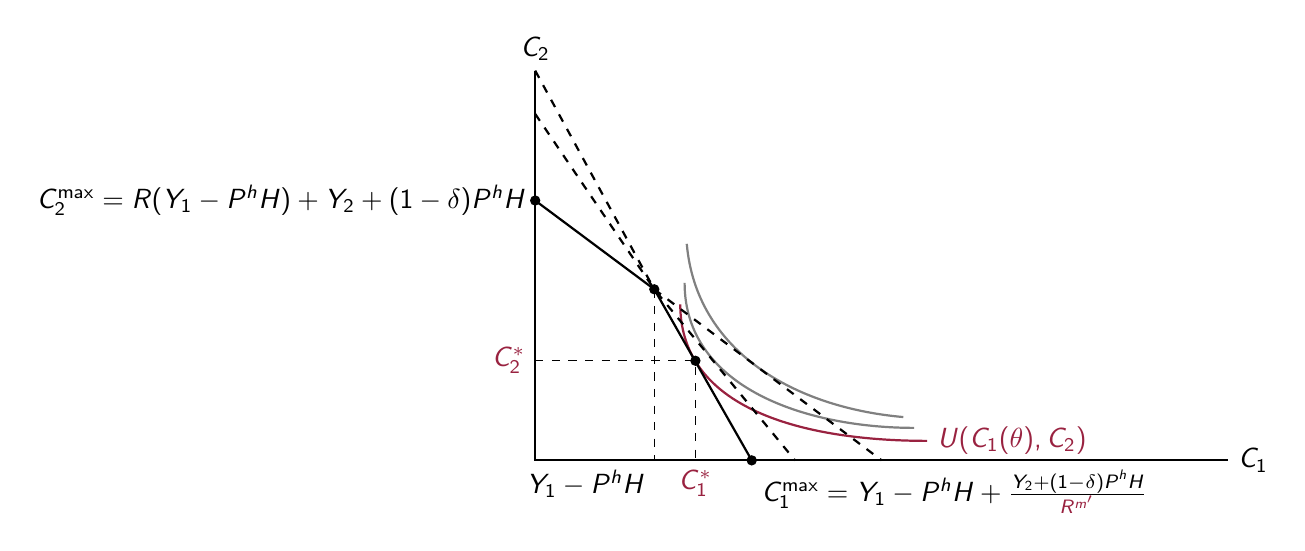
\begin{tikzpicture}[scale=0.55]
			\draw [thick,color=gray] (3.5,5) to [in=175,out=-85] (8.5,1);
			\draw [thick,color=gray] (3.45,4.1) to [in=180,out=-90] (8.75,0.75);
			\draw [thick,color=myred] (3.35,3.6) to [in=180,out=-90] (9.05,0.45) node [right]{\( U(C_1(\theta),C_2) \)};
			\draw [thick] (0,6) -- (2.75,3.95);
			\draw [thick, dashed] (2.75,3.95) -- (8,0);
			\draw [thick, dashed] (0,8) -- (2.75,3.95) -- (6,0);
			\draw [thick, dashed] (0,9) -- (2.75,3.95);
			\draw [thick] (2.75,3.95) -- (5,0);
			\draw [dashed] (2.75,3.95) -- (2.75,0) node [below left]{\( Y_1 - P^h H \)};
			\filldraw[black] (2.75,3.95) circle (3pt);
			\draw [dashed] (0,2.3) node [left,color=myred] {\( C_2^* \)}-- (3.7,2.3) -- (3.7,0) node [below,color=myred] {\( C_1^* \)};
			\filldraw[black] (3.7,2.3) circle (3pt);
			\filldraw[black] (0,6) circle (3pt) node [left]{\( C_2^\text{max} = R(Y_1 - P^h H) + Y_2 + (1-\delta)P^h H \)};
			\filldraw[black] (5,0) circle (3pt) node [below right]{\( C_1^\text{max} = Y_1 - P^h H + \frac{Y_2 + (1-\delta) P^h H}{\textcolor{myred}{R^{m'}}} \)};
			\draw [thick] (0,9) node[above]{\( C_2 \)} -- (0,0) -- (16,0) node [right]{\(C_1\)};
		\end{tikzpicture}
	\end{figure}
\subsubsection{Mortgage Finance Costs, Borrowing, and Consumption: Emperical Evidence}
	\begin{itemize}
		\item \textcolor{myblue}{How do borrowing and consumption respond to changes in mortgage interest rates?}
		\item Bhutta and Keys (2016) show that declining mortgage interest rates resulted in significant ``housing equity extraction'' in the form of ``cash out refinancing''
		\item They show that very little of the cash extracted was used to repay other debts
		\item Instead, the cash was used to finance consumption expenditures (e.g. cars, home renovation, holidays, etc)
	\end{itemize}
	\begin{figure}[H]
		\captionsetup[subfigure]{labelformat=empty}
		\centering
		\begin{subfigure}[t]{0.45\textwidth}
			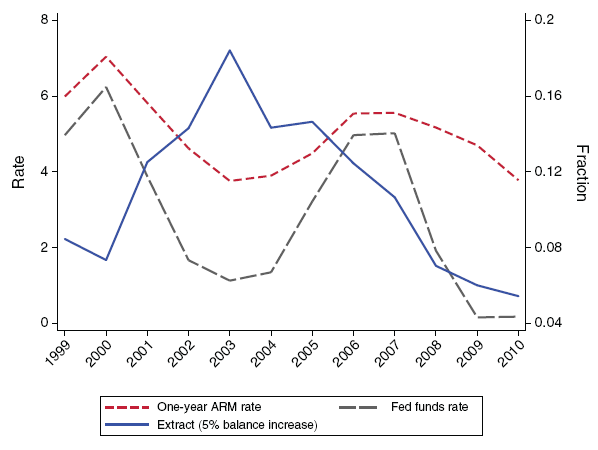
\includegraphics[width=\textwidth]{Figure 8.1.png}
			\caption{Probability of Extracting Equity in a Given Year versus Interest Rate}
		\end{subfigure}
		\hfill
		\begin{subfigure}[t]{0.45\textwidth}
			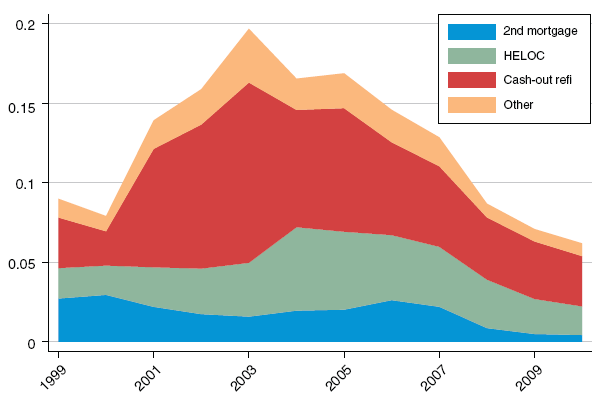
\includegraphics[width=\textwidth]{Figure 8.2.png}
			\caption{Method of Equity Extraction, by Year}
		\end{subfigure}	
	\end{figure}
	\textbf{Source:} Bhutta and Keys (2016) Interest Rates and Equity Extraction During the Housing Boom
\subsection{A Model of Constrained Mortgage Finance Decisions}
	\begin{itemize}
		\item Again consider a two period model where the homeowner has already chosen a house, \( H \)
		\item The house is purchased in period 1 at \( P_1^h \), and is sold in period 2 at price \( P_2^h \)
		\item Here, the homeowner is restricted in the amount that can be borrowed, \( B \)
		\begin{align*}
			\max_{C_1,C_2,B}\quad &\log C_1 + \beta\log C_2\\
			\text{s.t.}\quad &C_1+P_1^h H = Y_1 + B\\
			&C_2 + RB = Y_2 + (1-\delta) P_2^h H\\
			&B \leq \overline{\theta}P_1^h H
		\end{align*}
		\item The final inequality is a \textcolor{myblue}{loan to value constraint}
		\item The amount borrowed cannot exceed a fraction \( \overline{\theta} \) of the value of the house
		\item We can rewrite the budget constraints in terms of the LTV borrowing ratio \( \textcolor{myblue}{\overline{\theta} =\frac{B}{P_1^h H}} \)
		\item For period 1:
		\begin{align*}
			C_1+P_1^h H &= Y_1 + B\\
			C_1+P_1^h H &= Y_1 + \textcolor{myblue}{\frac{B}{P_1^h H}} P_1^h H\\
			C_1+P_1^h H &= Y_1 + \textcolor{myblue}{\overline{\theta}} P_1^h H
		\end{align*}
		\item For period 2:
		\begin{align*}
			C_2 + RB &= Y_2 + (1-\delta) P_2^h H\\
			C_2 + R\textcolor{myblue}{\frac{B}{P_1^h H}} P_1^h H &= Y_2 + (1-\delta) P_2^h \\
			C_2 + R\textcolor{myblue}{\overline{\theta}} P_1^h H &= Y_2 + (1-\delta) P_2^h H
		\end{align*}
		\item And where the LTV choice must be less than the maximum LTV: \( \textcolor{myblue}{\theta} \leq \overline{\theta} \)
		\item To illustrate the importance of the LTV constraint, we will make a figure in (\( \theta,C_2 \))-space
		\begin{itemize}
			\item This is similar to our previous figures in (\( C_1, C_2 \))-space
			\item \( \theta \) governs the amount borrowed, which has a direct effect on \( C_1 \)
		\end{itemize}
		\item Take the period 2 budget constraint:
		\[
			C_2 + R\textcolor{myblue}{\overline{\theta}} P_1^h H = Y_2 + (1-\delta) P_2^h H
		\]
		\item When the household borrows nothing, \( \textcolor{myblue}{\theta}=0 \) and maximum consumption is:
		\[
			C_2^\text{max} = Y_2 + (1-\delta)P_2^h H
		\]
		\item If there were no constraint on the LTV choice and \( C_2 = 0 \), then the maximum LTV would be:
		\[
			\textcolor{myblue}{\theta^\text{max}} = \frac{Y_2 + (1-\delta)P_2^h H}{RP_1^h H}
		\]
		\item Because of the LTV constraint \( (\theta\leq\overline{\theta}) \), the household is restricted in its borrowing
		\item This yields a truncated budget constrain in (\( \theta-C_2 \))-space
		\item Note: Higher \( \theta \) implies higher \( C_1 \), so the indifference curve is convex in (\( \theta-C_2 \))-space
		\item When constrained, consume more in period 2 and less in period 1 than if unconstrained
	\end{itemize}
	\begin{figure}[H]
		\centering
		\begin{tikzpicture}[scale=0.55]
			\draw [thick,gray] (3.5,5) to [in=175,out=-85] (8.5,1);
			\draw [thick,myblue] (3.05,4.5) to [in=175,out=-85] (8.75,0.75) node [right]{\( U(C_1(\theta),C_2) \)};
			\draw [thick] (0,6) -- (3.3,3.5);
			\draw [thick,dashed] (3.3,3.5) -- (8,0);
			\draw [dashed] (0,3.5) node [left] {\( C_2^* = Y_2 - R\overline{\theta}P_1^h H + P_2^h H (1-\delta)\)}-- (3.3,3.5) -- (3.3,0) node [below] {\( \overline{\theta} \)};
			\filldraw[black] (3.3,3.5) circle (3pt);
			\filldraw[black] (0,6) circle (3pt) node [left]{\( C_2^\text{max} = Y_2 + P_2^h H(1-\delta)\)};
			\filldraw[black] (8,0) circle (3pt) node [below]{\( \theta^\text{max} = \frac{Y_2+P_2^h H(1-\delta)}{RP_1^h H} \)};
			\draw [thick] (0,9) node[above]{\( C_2 \)} -- (0,0) -- (16,0) node [right]{\( \theta \)};
		\end{tikzpicture}
	\end{figure}
	\begin{itemize}
		\item Now consider a fall in the period 2 house price: \( P_2^h \rightarrow \textcolor{myred}{P_2^{h'}} \)
	\end{itemize}
	\begin{figure}[H]
		\centering
		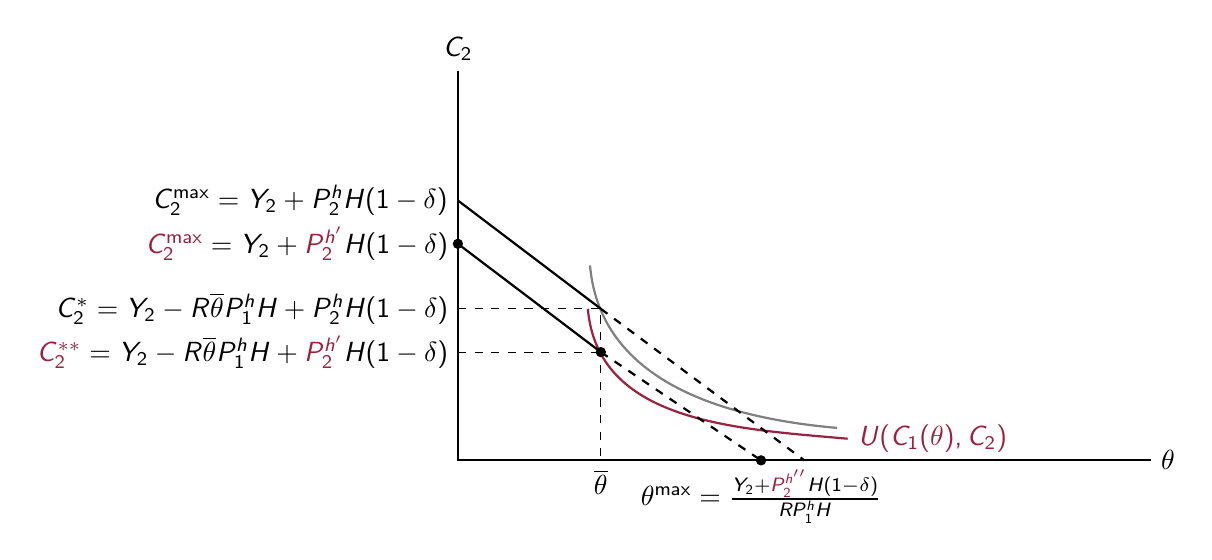
\begin{tikzpicture}[scale=0.55]
			\draw [thick,gray] (3.05,4.5) to [in=175,out=-85] (8.75,0.75);
			\draw [thick,myred] (3,3.5) to [in=175,out=-85] (9,0.5) node [right]{\( U(C_1(\theta),C_2) \)};
			\draw [thick] (0,6) node [left]{\( C_2^\text{max} = Y_2 + P_2^h H(1-\delta)\)} -- (3.3,3.5);
			\draw [thick,dashed] (3.3,3.5) -- (8,0);
			\draw [thick] (0,5) -- (3.3,2.5);
			\draw [thick,dashed] (3.3,2.5) -- (7,0);
			\draw [dashed] (0,3.5) node [left] {\( C_2^* = Y_2 - R\overline{\theta}P_1^h H + P_2^h H (1-\delta)\)}-- (3.3,3.5) -- (3.3,0) node [below] {\( \overline{\theta} \)};
			\draw [dashed] (0,2.5) node [left] {\( \textcolor{myred}{C_2^{**}} = Y_2 - R\overline{\theta}P_1^h H + \textcolor{myred}{P_2^{h'}} H (1-\delta)\)}-- (3.3,2.5);
			\filldraw[black] (3.3,2.5) circle (3pt);
			\filldraw[black] (0,5) circle (3pt) node [left]{\( \textcolor{myred}{C_2^\text{max}} = Y_2 + \textcolor{myred}{P_2^{h'}} H(1-\delta)\)};
			\filldraw[black] (7,0) circle (3pt) node [below]{\( \theta^\text{max} = \frac{Y_2+\textcolor{myred}{P_2^{h''}} H(1-\delta)}{RP_1^h H} \)};
			\draw [thick] (0,9) node[above]{\( C_2 \)} -- (0,0) -- (16,0) node [right]{\( \theta \)};
		\end{tikzpicture}
	\end{figure}
	\begin{itemize}
		\item What is the difference between \textcolor{myred}{constrained} vs. \textcolor{myblue}{unconstrained} households?
		\item The optimal consumption choices for each type of household are:
		\[
			C_2^\text{con} = Y_2 - R\overline{\theta}P_1^h H + (1-\delta)P_2^h H, \qquad C_2^\text{unc}=\frac{\beta R}{1 + \beta} \left(Y_1-P_1^h H + \frac{Y_2 + (1-\delta P_2^h H)}{R}\right)
		\]
		\item And the consumption responses to \( P_2^h \) are:
		\[
			\frac{\partial C_2^\text{con}}{\partial P_2^h} = (1-\delta) H, \qquad \frac{\partial C_2^\text{unc}}{\partial P_2^h} = \frac{\beta}{1+\beta}(1-\delta)H
		\]
		\item Constrained consumption much more sensitive than unconstrained consumption!
	\end{itemize}
\section{Housing Booms and Busts}
\subsection{A Simple Model of Mortgage Credit and Housing Booms and Busts}
	\begin{itemize}
		\item How do credit conditions affect the housing marker?
		\item Consider a simple model of a household that purchases housing using a mortgage
		\item The size of the mortgage is determined by credit conditions:
		\begin{itemize}
			\item The cost of borrowing, i.e. the interest rate
			\item The maximum Loan-to-Value constraint on mortgage borrowing
		\end{itemize}
		\item Housing market equilibrium:
		\begin{itemize}
			\item House prices adjust to ensure that housing demand equals housing supply
		\end{itemize}
		The household problem is:
		\begin{align*}
			\max_{C_t,C_{t+1},B_{t+1},H_{t+1}}\quad &u(C_t) + \beta[u(C_{t+1}) + v(H_{t+1})]\\
			\text{s.t.}\quad &C_t + P_t H_{t+1} = Y_t + B_{t+1}\\
			&C_{t+1} + (1+r_{t+1})B_{t+1} = Y_{t+1} + (1-\delta)P_{t+1}H_{t+1}\\
			&B_{t+1} \leq \theta_tP_tH_{t+1}
		\end{align*}
		\item Choose housing at time \( t \) to be enjoyed at time \( t+1 \)
		\item Sell housing at time \( t+1 \)
		\item Borrow \( B_{t+1} \) to finance housing, subject to a maximum LTV constraint
		\item Make three very useful simplifying assumptions:
		\begin{itemize}
			\item Linear utility in consumption: \( u(C) = C \)
			\item Log utlity in housing: \( v(H)=\log H \)
			\item Household is always constrained, i.e. always borrowing as much as allowed by the LTV constraint
		\end{itemize}
		\begin{align*}
			\max_{C_t,C_{t+1},B_{t+1},H_{t+1}}\quad &C_t + \beta[C_{t+1} + \log H_{t+1}]\\
			\text{s.t.}\quad &C_t + P_t H_{t+1} = Y_t + B_{t+1}\\
			&C_{t+1} + (1+r_{t+1})B_{t+1} = Y_{t+1} + (1-\delta)P_{t+1}H_{t+1}\\
			&B_{t+1} = \theta_tP_tH_{t+1}
		\end{align*}
		\item The Lagrangian function:
		\begin{align*}
			\mathcal{L} = C_t &+ \beta[C_{t+1} + \log H_{t+1}] + \lambda_t(Y_t + B_{t+1} - C_t - P_t H_{t+1})\\ 
			&+ \lambda_{t+1}(Y_{t+1} + (1-\delta)P_{t+1}H_{t+1} - C_{t+1} - (1+r_{t+1})B_{t+1}) + \mu_t(\theta_tP_tH_{t+1} - B_{t+1})
		\end{align*}
		\item \( \lambda_t,\lambda_{t+1} \) are Lagrange multipliers on the budget constraints
		\item \( \mu_t \) is the Lagrange multiplier on the LTV constraint
		\item The first order conditions are:
		\begin{align*}
			C_t:& \quad1=\lambda_t\\
			C_{t+1}:& \quad\beta=\lambda_{t+1}\\
			B_{t+1}:& \quad\lambda_t=\lambda_{t+1}(1+r_{t+1})+\mu_t\\
			H_{t+1}:& \quad\lambda_tP_t=\beta\frac{1}{H_{t+1}}+\lambda_{t+1}(1-\delta)P_{t+1}+\mu_t\theta_tP_{t+1}
		\end{align*}
		\item Combining the first order conditions, and repeating the LTV constraint, we have:
		\begin{align*}
			1-\mu_t&=\beta(1+r_{t+1}) \marginnote{Consumption Euler Equation}\\
			P_t&=\frac{\beta}{1-\mu_t\theta_t}\left( \frac{1}{H_{t+1}} + (1-\delta)P_{t+1} \right)\marginnote{Housing Euler Equation}\\
			B_{t+1}&=\theta_tP_tH_{t+1} \marginnote{LTV Constraint}
		\end{align*}
		\item Note \( \mu_t \) is the Lagrange multiplier on the borrowing constraint
		\item It tells us the marginal value of an extra dollar borrowed to finance housing
	\end{itemize}
\subsubsection{Housing Market Equilibrium}
	\begin{itemize}
		\item Housing market equilibrium:
		\[
			\underbrace{H_{t+1}}_\text{Housing Demand} = \underbrace{\overline{H}}_\text{Housing Supply}
		\]
		\item The house price \( p_t \) adjusts to ensure housing market clears in each period \( t \)
	\end{itemize}
\subsubsection{Model Experiment: Expansion of Mortgage Credit}
	\begin{itemize}
		\item First, find the \textcolor{myblue}{steady state} of the model
		\item Assume that all variables are the same forever eg. \( r_t=t_{t+1}=r \)
		\item Our model equations in the steady state are:
		\begin{align}
			1-\mu &= \beta(1+r) \label{E:10.1}\\
			P &= \frac{\beta}{1-\mu\theta} \left( \frac{1}{\overline{H}} + (1-\delta)P \right) \label{E:10.2}\\
			B &= \theta P\overline{H} \label{E:10.3}
		\end{align}
		\item Solve for the house price \( P \) (using \cref{E:10.1} and \cref{E:10.2}):
		\[
			P = \frac{\beta}{\overline{H}((1-\theta)(1-\beta)+\beta(\theta r+\delta))}
		\]
		\item Solve for mortgage debt (using \cref{E:10.3})
		\[
			B = \frac{\beta\theta}{((1-\theta)(1-\beta)+\beta(\theta r+\delta))}
		\]
		\item First, consider the effect of a \textcolor{myblue}{change in the interest rate \( \mathit{r} \)}
		\begin{align*}
			\frac{\partial P}{\partial r} &= -\overline{H}\beta\theta \times \frac{\beta}{(\overline{H}((1-\theta)(1-\beta)+\beta(\theta r+\delta)))^2} <0\\
			\frac{\partial B}{\partial r} &= -\beta\theta \times \frac{\beta\theta}{((1-\theta)(1-\beta)+\beta(\theta r+\delta))^2} <0
		\end{align*}
		\item Decrease in interest rates leads to: 1. \textcolor{myblue}{increase in house prices}; 2. \textcolor{myblue}{increase in mortgage debt}
		\begin{itemize}
			\item Lower mortgage finance costs increase housing demand
			\item With fixed housing supply \( \overline{H} \), prices must increase
			\item To finance higher-priced houses, households must increase borrowing
		\end{itemize}
		\item Second, consider the effect of a \textcolor{myblue}{change in the maximum LTV ratio \( \theta \)}
		\begin{align*}
			\frac{\partial P}{\partial\theta} &= -\overline{H}(1-\beta(1+r)) \times \frac{\beta}{(\overline{H}((1-\theta)(1-\beta)+\beta(\theta r+\delta)))^2} \\
			\frac{\partial B}{\partial\theta} &= \frac{\beta\theta}{((1-\theta)(1-\beta)+\beta(\theta r+\delta))} + (1-\beta(1+r)) \times \frac{\beta\theta}{((1-\theta)(1-\beta)+\beta(\theta r+\delta))^2}
		\end{align*}
		\item If \( \beta(1+r) > 1 \), households are patient and/or have high costs of borrowing
		\begin{itemize}
			\item Demand for housing does not rise with increased borrowing opportunities
			\[
				\frac{\partial P}{\partial \theta} <0, \qquad \frac{\partial B}{\partial \theta} <0 
			\]
		\end{itemize}
		\item If \( \beta(1+r) < 1 \), households are impatient and/or have with costs of borrowing
		\begin{itemize}
			\item Demand for housing rises with increased borrowing opportunities
			\item Seems most likely case since we observe households borrow a lot to finance housing
			\[
				\frac{\partial P}{\partial \theta} >0, \qquad \frac{\partial B}{\partial \theta} >0 
			\]
		\end{itemize}
	\end{itemize}
\subsection{Dynamics of Mortgage and Housing Markets}
\subsubsection{Dynamic Model Experiment: Expansion of Mortgage Credit}
	\begin{itemize}
		\item Now study the \textcolor{myblue}{dynamics} of the model in response to an expansion of mortgage credit
		\item We will consider effect of our two shocks:
		\begin{enumerate}[label=\textbf{\arabic*.}]
			\item A decrease in the mortgage interest rate
			\item An increase in the maximum LTV ratio on mortgage borrowing
		\end{enumerate}
		\item Recall the FOCs/optimal decisions of the household:
		\begin{align*}
			1-\mu_t&=\beta(1+r_{t+1}) \marginnote{Consumption Euler Equation}\\
			P_t&=\frac{\beta}{1-\mu_t\theta_t}\left( \frac{1}{H_{t+1}} + (1-\delta)P_{t+1} \right) \marginnote{Housing Euler Equation}\\
			B_{t+1}&=\theta_tP_t\overline{H} \marginnote{LTV Constraint}
		\end{align*}
		\item To begin, suppose ``beliefs'' about future house prices are held fixed: \( P_{t+1} = P \)
		\item Trace out effect of a decline in \textcolor{myblue}{\( r_{t+1} \)}
		\begin{align*}
			1-\underbrace{\textcolor{myblue}{\mu_t}}_\uparrow&=\beta(1+\underbrace{\textcolor{myblue}{r_{t+1}}}_\downarrow) \marginnote{Consumption Euler Equation}\\
			\underbrace{\textcolor{myblue}{P_t}}_\uparrow&=\frac{\beta}{1-\underbrace{\textcolor{myblue}{\mu_t}}_\uparrow\theta_t}\left( \frac{1}{H_{t+1}} + (1-\delta)P_{t+1} \right) \marginnote{Housing Euler Equation}\\
			\underbrace{\textcolor{myblue}{B_{t+1}}}_\uparrow1&=\theta_t\underbrace{\textcolor{myblue}{P_t}}_\uparrow H_{t+1} \marginnote{LTV Constraint}
		\end{align*}
		\begin{itemize}
			\item Lower interest rates \( \Rightarrow \) increase marginal utility of extra dollar borrowed
			\item Increased demand for housing \( \Rightarrow \) with fixed supply, current prices must rise
			\item Borrowing increases to pay for higher price of houses
		\end{itemize}
		\item Trace out effect of a rise in \textcolor{myred}{\( \theta_t \)}:
		\begin{align*}
			1-\mu_t&=\beta(1+r_{t+1}) \marginnote{Consumption Euler Equation}\\
			\underbrace{\textcolor{myred}{P_t}}_\uparrow&=\frac{\beta}{1-\mu_t\underbrace{\textcolor{myred}{\theta_t}}_\uparrow}\left( \frac{1}{H_{t+1}} + (1-\delta)P_{t+1} \right) \marginnote{Housing Euler Equation}\\
			\underbrace{\textcolor{myred}{B_{t+1}}}_\uparrow&=\underbrace{\textcolor{myred}{\theta_t}}_\uparrow\underbrace{\textcolor{myred}{P_t}}_\uparrow\overline{H} \marginnote{LTV Constraint} 
		\end{align*}
		\begin{itemize}
			\item Higher LTV borrowing limits \( \Rightarrow \) increase amount that can be borrowed
			\item Since households always borrow as much as they can, borrowing increases
			\item Demand for housing increases in line with borrowing \( \Rightarrow \) with fixed supply, prices rise
		\end{itemize}
		\item Now to solve the model in practice (e.g. on a computer!)
		\item Create \textbf{exogenous} paths (i.e shocks) for \( r_{t+1} \) and \( \theta_t \)
		\item Assume model is in new steady state at some point in the future (e.g. some period \textit{T})
		\item Iterating backwards from \textit{T}, take \( P_{t+1} \) as given, then solve for \( P_t,B_{t+1} \):
		\begin{align*}
			1- \mu_t &= \beta(1+r_{t+1}) \\
			P_t &= \frac{\beta}{1-\mu_t\theta_t}\left( \frac{1}{H} + (1-\delta)P_{t+1} \right)\\
			B_{t+1} &= \theta_tP_t\overline{H}
		\end{align*}
		\item For our dynamic experiments:
		\begin{itemize}
			\item The shocks last for 8 quarters (i.e. two years)
			\item The shocks are unanticipated each period (i.e. a complete surprise)
			\item We run experiments separately for: (1) interest rate shocks, (2) LTV ratio shocks, (3) both interest rates and LTV ratio shocks
		\end{itemize}
	\end{itemize}
	\begin{figure}[H]
		\centering
		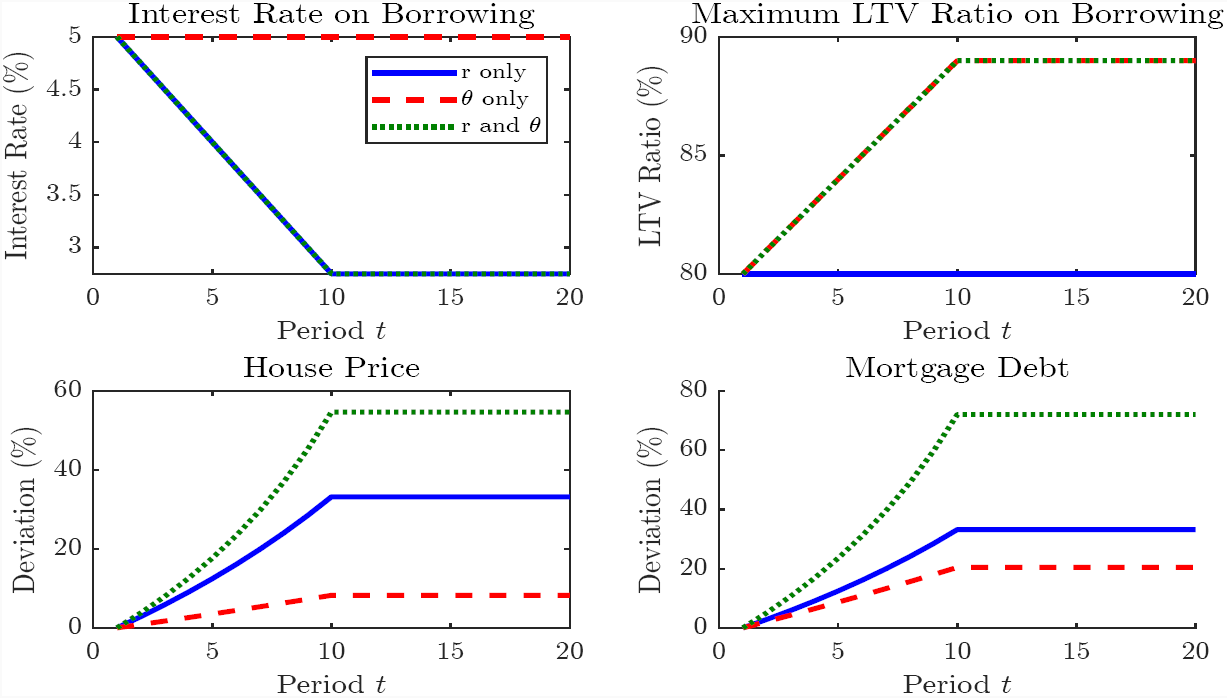
\includegraphics[scale=0.4]{Figure 11.1}
	\end{figure}
	\begin{itemize}
		\item The boom is the same as our previous experiment
		\begin{itemize}
			\item Each model period represents 1 quarter
			\item The credit expansion shock lasts for 8 quarters (i.e. two years)
			\item The shocks are unanticipated each period (i.e. a complete surprise)
		\end{itemize}
		\item But now for the credit bust shock:
		\begin{itemize}
			\item In the 9th quarter, interest rates and the LTV ratio revert to their initial steady state values in just 4 quarters (i.e. one year)
		\end{itemize}
	\end{itemize}
	\begin{figure}[H]
		\centering
		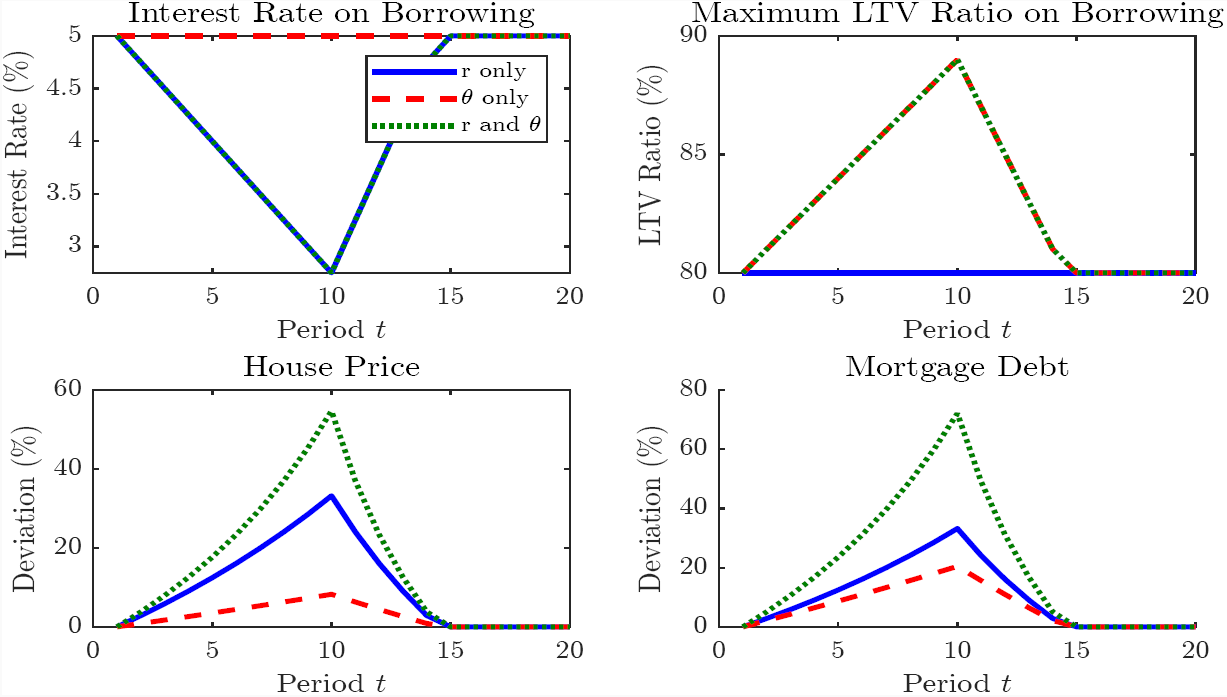
\includegraphics[scale=0.4]{Figure 11.2}
	\end{figure}
\section{Welfare and Redistribution Through Asset Price Movements}
\subsection[A Simple Model]{A Simple Model of Welfare Gains and Losses From Asset Price Movements}
	\begin{itemize}
		\item Simple model of asset choice and asset price movements
		\item Hold initial asset stock, rebalance asset portfolio, earn cash flow next period
		\item A household's problem is:
		\begin{align*}
			\underbrace{V}_\text{\textcolor{myblue}{Value Function}} = &\max_{C_1,C_2,A_2}U(C_1)+\beta U(C_2)\\
			\text{s.t}\quad &C_1+(A_2-A_1)P_1=Y_1\\
			&C_2 = Y_2+A_2D_2
		\end{align*}
		\item where:
		\begin{itemize}
			\item \( P_1= \) price of asset when buying/selling at time 1
			\item \( D_2= \) cash flow/dividends from asset at time 2
			\item \( (A_2-A_1)= \) \text{net transactions of the asset in period 1} 
			\item \( V= \) \textcolor{myblue}{Value Function}, the total utility of the consumption and asset choices for the household
		\end{itemize}
		\item The Lagrangian equation is:
		\[
			\mathcal{L} = U(C_1) + \beta U(C_2) + \lambda_1(Y_1-C_1-(A_2-A_1)P_1) + \lambda_2(Y_2+A_2D_2-C_2)
		\]
		\item The first order conditions are:
		\begin{align*}
			C_1: \quad &Y'(C_1) = \lambda_1\\
			C_2: \quad &\beta U'(C_2) = \lambda_2\\
			A_2: \quad &\lambda_1P_1=\lambda_2D_2
		\end{align*}
		\item And, combining the FOCs, we find the Euler equation:
		\[
			\underbrace{U'(C_1)}_{\text{Marginal Utility of }C_1} = \underbrace{\beta U'(C_2)}_{\text{Marginal Utility of }C_2} \times \underbrace{\frac{D_2}{P_1}}_\text{Return on asset}
		\]
		\item Recall, Euler equation describes optimal inter-temporal decisions of the household
		\item Characterises trade-off between consumption today and investment for consumption tomorrow
		\item Note that the price of the asset \textcolor{myblue}{\( P_1 \)} directly affects asset returns \textcolor{myblue}{\( \frac{D_2}{P_1} \)}
		\item All else equal, higher prices reduce returns which discourages further investment in the asset
		\item But asset price \textcolor{myred}{\( P_1 \)} has \textbf{indirect} effects through valuation of household wealth
		\item Recall the period 1 budget constraint is:
		\[
			C_1=Y_1 + \underbrace{\textcolor{myred}{P_1A_1}-P_1A_2}_\text{Net change in asset position}
		\]
		\item E.g. an increase in the price \( P_1 \) increases the value of the households initial portfolio: \( P_1A_1 \)
		\item This change in portfolio values is called the \textcolor{myred}{wealth effect}
		\item We want to understand the \textcolor{myblue}{welfare} gains/losses from a change in asset prices
		\item Overall, are households better off or worse off when asset prices rise?
		\item Depends on size of effects on returns and \textcolor{myred}{wealth}
		\begin{itemize}
			\item Higher asset prices reduce asset returns, making households worse off
			\item Higher asset prices increase value of initial wealth, making households better off
		\end{itemize}
		\item What is the effect of an increase in asset prices \( P_1 \)?
		\begin{align*}
			\frac{\partial V}{\partial P_1} &= \frac{\partial U(C_1)}{\partial C_1} \times \frac{\partial C_1}{\partial P_1} + \frac{\partial U(C_2)}{\partial C_2} \times \frac{\partial C_2}{\partial P_1}\\
			&= U'(c_1) \times (A_1-A_2)
		\end{align*}
		\item Where \( (A_1-A_2) \) is net asset portfolio transactions
		\item Another way to understand this: rewrite the budget constraint as:
		\item And the budget constraints:
		\begin{align*}
			C_1 &= Y_1 + (A_1-A_2) P_1 \\
			&= Y_1 + \frac{P_1}{P_0}P_0A_1 - \frac{P_1}{D_2}D_2A_2 \\
			&= Y_1 + R_1P_0A_1 - \frac{1}{R_2}D_2A_2
		\end{align*}
		\item Where \( P_0 \) is the initial price assets were purchased at, \( R_1 \) is the return on assets bought prior to time 1, and \( R_2 \) is the return on assets purchased at time 1
		\item Now what is the effect of an increase in asset prices \( P_1 \)?
		\begin{align*}
			\frac{\partial V}{\partial P_1} &= \frac{\partial U(C_1)}{\partial C_1} \times \left( \underbrace{\frac{\partial C_1}{\partial R_1} \times \frac{\partial R_1}{\partial P_1}}_\text{Wealth effect}\quad + \underbrace{\frac{\partial C_1}{\partial R_2} \times \frac{\partial R_2}{\partial P_1}}_\text{Investment returns effect} \right)\\
			&= \underbrace{U'(C_1) \times A_1P_0 \times \frac{\partial R_1}{\partial P_1}}_\text{Wealth effects} + \underbrace{U'(C_1) \times A_2D_2 \times A_1^{-2} \times \frac{\partial R_1}{\partial P_1}}_\text{Investment returns effect}
		\end{align*}
		\item Changes in \( P_1 \) may have different implications for welfare via returns:
		\begin{itemize}
			\item Higher \( P_1 \) increases returns in period 1 (i.e. a \textcolor{myred}{wealth effect})
			\item Higher \( P_1 \) increases returns in period 2 (holding \( D_2 \) constant)
		\end{itemize}
		\item Important! Overall effect on \textcolor{myblue}{welfare} is not the same as \textcolor{myred}{wealth effect}
		\begin{itemize}
			\item \textcolor{myblue}{Welfare effect} = \( \frac{\partial V}{\partial P_1} \)
			\item \textcolor{myred}{Wealth effect} = \( U'(C_1) \times A_1P_0 \times \frac{\partial R_1}{\partial P_1} \)
		\end{itemize}
		\item The \textcolor{myblue}{welfare effect} of asset price movements is summarised by:
		\[
			U'(c_1) \times (A_1-A_2)
		\]
		\item First, consider a \textbf{net seller} of assets: \( A_1 > A_2 \)
		\[
			\frac{\partial V^{seller}}{\partial P_1} = U'(C_1) \times (A_1 - A_2) > 0
		\]
		\item Earn higher returns on assets sold, net gain
		\item Second, consider a \textbf{net buyer} of assets: \( A_1 < A_2 \)
		\[
			\frac{\partial V^{buyer}}{\partial P_1} = U'(C_1) \times (A_1 - A_2) < 0
		\]
		\item Earn lower returns on asset investments, net loss
	\end{itemize}
\subsubsection{Graphical Illustration}
	\begin{itemize}
		\item Increase in \( P_1 \) tilts budget constraint out
		\item Can spend down more net asset wealth
		\item For \textbf{net seller} of assets, consume more in both periods
		\item Higher indifference curve \( \Leftrightarrow \) higher utility \( \Leftrightarrow \) higher welfare
	\end{itemize}
	\begin{marginfigure}
		\centering
		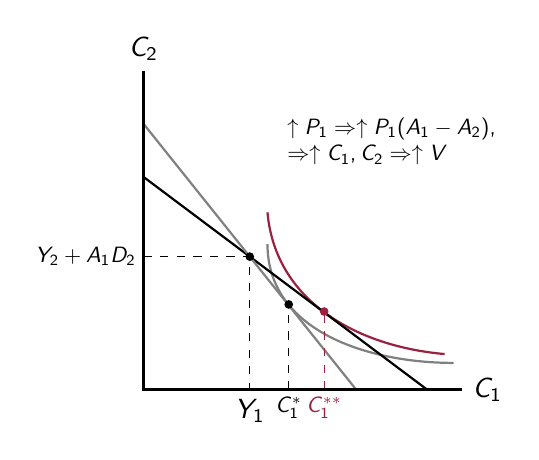
\begin{tikzpicture}[scale=0.45]
			\draw [thick,color=myred] (3.5,5) to [in=175,out=-85] (8.5,1);
			\draw [thick,color=gray] (3.5,4.1) to [in=180,out=-90] (8.75,0.75);
			\draw [thick] (0,6) -- (8,0);
			\draw [thick,color=gray] (0,7.5) -- (6,0);
			\draw [dashed] (0,3.75) node[left,scale=0.8]{\( Y_2 + A_1D_2 \)} -- (3,3.75) -- (3,0) node[below]{\( Y_1 \)};
			\filldraw[black] (3,3.75) circle (3pt);
			\draw [dashed] (4.1,0) node[below,scale=0.8]{\( C_1^* \)} -- (4.1,2.4);
			\filldraw[black] (4.1,2.4) circle (3pt);
			\draw [dashed,myred] (5.1,0) node[below,scale=0.8]{\( C_1^{**} \)} -- (5.1,2.2);
			\filldraw[myred] (5.1,2.2) circle (3pt);
			\node [scale=0.8,align=left] at (7,7){\( \uparrow P_1\Rightarrow\uparrow P_1(A_1-A_2)\),\\\(\Rightarrow\uparrow C_1,C_2 \Rightarrow \uparrow V \)};
			\draw [thick] (0,9) node[above]{\( C_2 \)} -- (0,0) -- (9,0) node [right]{\(C_1\)};
		\end{tikzpicture}
		\caption{Higher indifference curve}\label{fig:11.1}
	\end{marginfigure}
	\begin{itemize}
		\item Increase in \( P_1 \) tilts budget constraint out
		\item Investment in net assets is more expensive
		\item For \textbf{net buyer} of assets, consume less in both periods
		\item Lower indifference curve \( \Leftrightarrow \) lower utility \( \Leftrightarrow \) lower welfare
	\end{itemize}
	\begin{marginfigure}
		\centering
		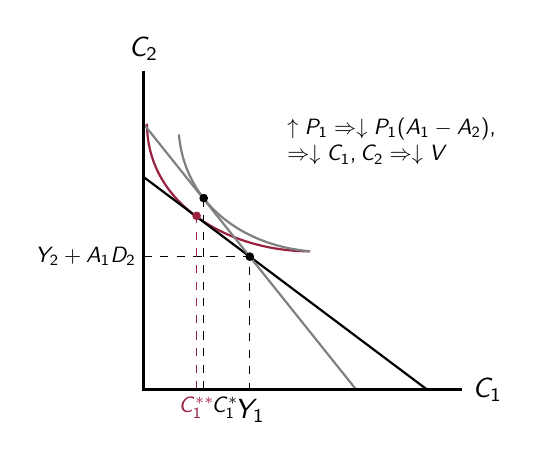
\begin{tikzpicture}[scale=0.45]
			\draw [thick,color=myred] (0.1,7.5) to [in=180,out=-90] (4.7,3.9);
			\draw [thick,color=gray] (1,7.2) to [in=175,out=-85] (4.7,3.9);
			\draw [thick] (0,6) -- (8,0);
			\draw [thick,color=gray] (0,7.5)-- (6,0);
			\draw [dashed] (0,3.75) node[left,scale=0.8]{\( Y_2 + A_1D_2 \)} -- (3,3.75) -- (3,0) node[below]{\( Y_1 \)};
			\filldraw[black] (3,3.75) circle (3pt);
			\draw [dashed,myred] (1.5,0) node[below,scale=0.8]{\( C_1^{**} \)} -- (1.5,4.9);
			\filldraw[myred] (1.5,4.9) circle (3pt);
			\draw [dashed] (1.7,0) node[below right,scale=0.8]{\( C_1^* \)} -- (1.7,5.4);
			\filldraw[black] (1.7,5.4) circle (3pt);
			\node [scale=0.8, align=left] at (7,7){\( \uparrow P_1\Rightarrow\downarrow P_1(A_1-A_2)\),\\\(\Rightarrow\downarrow C_1,C_2 \Rightarrow \downarrow V \)};
			\draw [thick] (0,9) node[above]{\( C_2 \)} -- (0,0) -- (9,0) node [right]{\(C_1\)};
		\end{tikzpicture}
		\caption{Lower indifference curve}\label{fig:11.2}
	\end{marginfigure}
\end{document}
